\documentclass[a4paper]{article} % A4 paper and 11pt font size

\usepackage{braket}
\usepackage{amsmath}
\usepackage{amssymb}
\usepackage{bm}
\usepackage[utf8]{inputenc}
\usepackage{verbatim}
\usepackage{tikz}
%\usepackage{pgfornament}
\usepackage{pgfplots}
\usepackage{pgffor}
\usepackage[version-1-compatibility]{siunitx}
\usepackage{fancyhdr}
\usepackage{lipsum}
\usepackage{gensymb}
\usepackage{framed}
\usepackage{cancel}
\usepackage{slashed}
\usepackage{hyperref}
\usepackage{pdflscape}
\usepackage{graphicx}
\usepackage{caption}
\usepackage{subcaption}
\usepackage{geometry}
\usepackage{yfonts}
\usepackage{calc}
\usepackage{cite}
\usepackage{siunitx}
\usepackage{mathtools} %for underbraces without whitespace (\mathclap{})

\newcommand{\utilde}[1]{\tilde{#1}}

\newcommand{\vect}[1]{\mathbf{#1}} %3D vector
\renewcommand{\div}{\text{div}~}
\newcommand{\diag}{\text{diag}~}
\newcommand{\ph}[1]{\phantom{#1}}

\setlength{\parindent}{0em}
\setlength{\parskip}{1em}
\newcommand{\goth}[1]{{\Huge\textfrak{#1}}}
\renewcommand{\baselinestretch}{1.1}

\newcommand{\exercise}[2]
{
\begin{framed}
\textbf{Exercise:} #1 \\\hrule
#2
\end{framed}
}

\newcommand{\example}[2]
{
\begin{framed}
\textbf{Example #1:} #2
\end{framed}
}

\newcommand{\review}[1]
{
\hrule
A short review:

#1
\hrule
}

\renewcommand{\picture}[1]
{
\begin{figure}[h]
\centering
\includegraphics[width=0.5\textwidth]{#1}
\end{figure}
}

\newcommand{\picturesize}[2]
{
\begin{figure}[h]
\centering
\includegraphics[width=#2\textwidth]{#1}
\end{figure}
}

\newcommand{\bmx}[1]{
\begin{bmatrix}
#1
\end{bmatrix}
}

\newcommand{\pmx}[1]{
\begin{pmatrix}
#1
\end{pmatrix}
}

\renewcommand{\tilde}{\widetilde}

 \geometry{
 a4paper,
 total={210mm,297mm},
 left=28mm,
 right=28mm,
 top=30mm,
 bottom=40mm,
 }


%----------------------------------------------------------------------------------------
%	TITLE SECTION
%----------------------------------------------------------------------------------------
%\setlength\parindent{0pt} % Removes all indentation from paragraphs - comment this line for an assignment with lots of text


\pagenumbering{arabic}
\begin{document}
\pagestyle{empty}

\newcommand{\HRule}{\rule{\linewidth}{0.5mm}}

\begin{titlepage}

    \begin{center}
        \textsc{\large SN: 587623}\\[6cm]

        \HRule \\[0.5cm]
		\Huge \textbf{PHYC90012 General Relativity}\\[0.5cm]
        \huge \textbf{Course Summary}\\[0.5cm] 
        \HRule \\[1.5cm]
        \begin{minipage}{0.4\textwidth}
        \begin{center}

        \large By \\[0.75cm]
        \huge Braden \scshape Moore \\[0.5cm]
        \normalsize \normalfont Master of Science \\
        The University of Melbourne \\

        \end{center}
        \end{minipage}

        \vfill

        \large \today
    \end{center}


\newpage
\end{titlepage}
%----------------------------------------------------------------------------------------
\pagestyle{empty}
\tableofcontents
\newpage

\pagestyle{fancy}
\pagenumbering{arabic}
\rfoot{\textsc{Braden Moore, 587623}}
\lfoot{\textsc{\today}}
\lhead{\textsc{Semester 1, 2016}}
\rhead{\textsc{PHYC90012 General Relativity}}
\setcounter{page}{1}
\setcounter{section}{-1}
\section{Syllabus}
\subsection{Part I}
\begin{enumerate}
\item Introduction to gravity
\begin{itemize}
\item Order of magnitude estimates
\item Small amount of quantum gravity
\end{itemize}
\item Equivalence principle
\item Experimental foundations
\item Geometric objects
\begin{itemize}
\item Need to understand geometric components of GR
\item Vectors, metric, etc. that live on manifolds
\item Laws of nature do not depend on coordinates chosen
\item Hence can write laws of nature in terms of geometric objects w/o reference to coordinates
\end{itemize}
\item Kinematics
\begin{itemize}
\item Time dilation, length contraction in GR framework
\end{itemize}
\item Calculus in curvilinear coordinates
\begin{itemize}
\item Mass and energy curve space time
\item Hence geometric objects moved on curved manifolds
\item Distances are not only spatial but temporal; need to use mathematics of small change = calculus
\item Uses the covariant derivative (a geometric object; independent of basis/coordinate independent)
\item This point of the course we will not be considering curved space, but instead only curvilinear coords 
\begin{itemize}
\item A flat space can be covered (represented?) by curved coordinates, but an intrinsically curved surface cannot be covered by flat coordinates
\end{itemize}
\end{itemize}
\item Curved spaces
\begin{itemize}
\item Manifolds 
\item How to calculate lengths, volumes, angles in curved spaces
\item Introduces the idea of parallel transport $\Rightarrow$ leads to curvature
\item Define the Riemann tensor, and its children etc. Ricci tensor, ...; these satisfy the Bianchi identities
\end{itemize}
\item Einstein's field equations
\begin{itemize}
\item Stress-energy tensor
\end{itemize}
\item Weak-field limit
\begin{itemize}
\item Gauge transformations
\end{itemize}
\subsection{Part II - Applications}
\item GR phenomena revisited 
\begin{itemize}
\item GPS, Mercury's orbit, gravitational lensing, gravitational redshift, ...
\end{itemize}
\item Gravitational waves
\begin{itemize}
\item Propagation (phase speed, polarisation, ...)
\item Generation*
\item Detection*
\begin{itemize}
\item[*] = together these form the ``antenna problem"
\end{itemize}
\end{itemize}
\item Relativistic stars
\begin{itemize}
\item neutron stars
\item equation of state (cannot study on Earth because largest nuclei only have 200 elements or so; need more density)
\end{itemize}
\item Black holes
\begin{itemize}
\item Event horizons, singularities, ...
\end{itemize}
\item Cosmology
\begin{itemize}
\item Friedman-Robertson-Walker (FRW) metric - describes a homogeneous, isotropic universe
\begin{itemize}
\item We will derive this and the Friedman equations
\end{itemize}
\end{itemize}

\end{enumerate}

\pagebreak

\part{Theoretical tools of the trade}


\section{Introduction to gravity}
\subsection{Strength of gravity}
\begin{itemize}
\item Weak! Weakest of all fundamental forces
\item Long-ranged force (like EM)
\item Weakness determined by coupling constant
\item Coupling constant = Newton's gravitational constant
\end{itemize}
\begin{equation}
\vec{F}=\frac{Gm_1 m_2}{r_{12}^2}\hat{r}
\end{equation}
\begin{itemize}
\item G is hard to measure; least well known of coupling constants
\end{itemize}
In 1797-98, Cavendish used torsion balls (1.8m torsion balance) with rod of big masses and rod of small masses. 
\begin{itemize}
\item Spring constant of torsion balance was measured from free oscillation
\item then introduced 158kg balls
\item measured deflection angle of balance $\Rightarrow$ can calculate force
\begin{itemize}
\item using a mini-telescope against Vernier scale
\end{itemize}
\item rearrange Newton's law to get G
\end{itemize}

\picture{images/cavendish-torsion-balance.png}
 
\exercise{Show that Cavendish also measured density of Earth as a bonus at the same time.}
{Mass of Earth $M_{\oplus}= \rho V$ where $V=\frac{4}{3}\pi R^3$ assuming the Earth is a sphere. How does calculating $G$ also calculate $\rho$? Well, we have $\vec{F}=\frac{Gm_1 m_2}{r_{12}^2}\hat{r}$. Let's take $m_1 = M_\oplus$ as the mass of the Earth, and $m_2 = m$ as some small object mass. Let's imagine the smaller object falling to the center of the Earth. We'll take $r_{12}$ as the distance from the object to the Earth's center, which we can approximate as Earth's radius, i.e. $r_{12}=R$. This force should be equivalent to $F=ma$.\\
\\
So we have
\begin{align*}
\frac{GM_\oplus m}{R^2}&=mg\\
\frac{G\rho \frac{4}{3}\pi R^3}{R^2}&=g\\
\frac{4G \rho \pi R}{3}&=g\\
\Rightarrow \rho &=\frac{3g}{4\pi GR}\\
&=\frac{3\times \SI{9.8}{ms^{-2}}}{4\pi\times \SI{6.67384d-11}{\kg^{-1}\m^3 \s^{-2}}\times \SI{6370}{km}}\\
&=\frac{3\times 9.8}{4\pi\times 6.67384\times 10^{-11}\times 6370\times 10^3}\si{\kg.m^{-3}}\\
&=\SI{5503}{kg.m^{-3}}
\end{align*}
}


\begin{itemize}
\item Modern $G=6.67384(80)\times \SI{d-11}{Nm^{-2}.\kg^{-2}}=\si{\kg^{-1}.\m^3.\s^{-2}}$
\item Product GM is known to 1 part in $\sim 10^{10}$ from astrophysics observations
\begin{itemize}
\item[$\Rightarrow$] mass is hard to measure gravitationally
\end{itemize}
\item We need a dimensionless number to characterise strength
\item Newton: $\Phi=\frac{GM}{r}$ (potential)
\item In free fall: $\frac{KE}{mass}$, $v^2 \sim \frac{GM}{r}$
\item We claim gravity is strong is free-fall is relativistic, i.e. $v\sim c$
\item This is an order of magnitude estimate
\end{itemize}


\subsection{Strong vs. weak gravity}
\begin{itemize}
\item Quasi-Newtonian:
\begin{itemize}
\item characteristic speed of body in free fall: $v^2\sim \frac{GM}{r}$
\end{itemize}
\item Strong gravity leads to relativistic free fall, i.e. $\frac{GM}{Rc^2}\geq 1$ where M is the total mass and R is th characteristic size
\end{itemize}

\begin{table}
\centering
\begin{tabular}{c|cc} 
 & $\frac{GM}{Rc^2} \lll 1$ & $\frac{GM}{Rc^2}\geq 1$\\
\hline $v \ll c$ & Newtonian & CAN'T EXIST \\
$v\sim c$ & special rel. & full GR (difficult)
\end{tabular}
\end{table}

\example{1.1}{
$M=M_{\odot}$ (mass of the Sun)
\begin{align*}
R & \sim \frac{GM}{c^2} \text{\quad boundary of strong regime}\\
&\sim \frac{10^{-10}10^{30}}{10^{17}}\\
&\sim \text{km}
\end{align*}
cf. Schwarz radius of black hole $=\frac{2GM}{c^2}$
}
\example{1.2}{
Density of black hole with mass of $M_\odot$
\begin{align*}
&\sim \frac{M}{R^3}\sim\frac{\SI{d30}{kg}}{\si{(km)^3}}\\
&\sim 10^{21}kgm^{-3}
\end{align*}
How does this density compare to maximum density of (say) nuclear matter? Let's compare.
\begin{align*}
\frac{m_n}{(1fm)^3}\sim \frac{10^{-27}kg}{10^{-45}m^3}\sim 10^{18}kgm^{-3}
\end{align*}
We see a black hole is more dense that a nuclei. The characteristic size of a particle $1fm\sim\Delta x\sim \frac{\hbar}{\Delta p}\sim \frac{\hbar}{m_n c}$, due to Heisenberg's uncertainty principle, and also the Pauli exclusion principle.
}
More generally: density of material that forms black hole $\sim\frac{M}{R^3}$, but note $M=\frac{c^2R}{G}$ density $\rho \propto \frac{1}{R^2}$. This means that denser black holes are smaller.

\exercise{Estimate the strength of gravity $\frac{GM}{Rc^2}$ on Earth.}

\example{2}
{
The Universe is composed of 5\% baryons + 25\% dark matter + 70\% dark energy. Estimate M and R.\\\hrule
$R\sim \SI{10}{Gpc}$
\begin{itemize}
\item Mass of baryons 
\begin{itemize}
\item $10^{11}$ stars in Milky Way
\item $(10^4)^3$ galaxies in Universe
\item[$\Rightarrow$] $M_{\text{baryons}}\sim10^{23}M_\odot\sim \SI{d53}{kg}$
\end{itemize}
\end{itemize} 
\begin{equation}
\frac{GM_{tot}}{Rc^2}\sim\frac{10^{-10}\cdot 10^{53}\cdot 10}{10^{27} \cdot 10^{17}}\sim 1
\end{equation}
\begin{align*}
\text{Density }\rho\sim\frac{M_{tot}}{R_{tot}^3}&\sim\frac{c^2}{R^2G}\text{, use }\frac{GM}{Rc^2}\sim 1\\
&\sim\frac{1}{G\times(\text{age of universe})^2}
\end{align*}
cf. critical density from Friedmann equations $\rho_{crit}=\frac{3H_0^2}{8\pi G}$.\\
Recall Hubble constant $H_0\sim \frac{1}{\text{age}}$.
}
The critical density is the density of the universe at which expansion will asymptotically slow. Too dense leads to big crunch, too low leads to unbounded expansion.
\exercise{How do we reconcile a ``flat" universe from critical density with the ``curved" universe?}

Important to remember: gravity is strong when $\frac{GM}{Rc^2}\sim 1$, which occurs around black holes, the universe at large. In a sense, cosmological results such as critical density, expansion of universe come from this.

\subsection{Black hole oscillations}
We can estimate the oscillation frequency of a ``black hole'' (i.e. something with $\frac{GM}{Rc^2}\sim 1$ as $\sim \frac{c}{R}$; that is, the time is takes light to travel the distance of the object. This is the natural frequency for this object. Using that ubiquitous expression we can express the oscillation frequency as $\sim \frac{c^3}{GM}$, e.g. $M=M_\odot \Rightarrow \text{frequency}\sim\SI{10}{kHz}$.

Let's discuss charged black holes. It is difficult to astrophysically have charged black holes, because stars are not usually charged (due to the strength of the EM force, which would attract opposite charge and cancel out). So, these are artificial in nature. These have unusual geometry, and are called ``Reissner-Nordstrom'' black holes.
\example{}{What is the maximum charge on a black hole?\\\hrule
\begin{align*}
\frac{Q^2}{4\pi\epsilon_0 R}&\leq \frac{GM^2}{R}\\
Q&\leq (4\pi\epsilon_0 G)^{1/2} M
\end{align*}
Above, we relate Coloumb force to gravitational force. The gravitational force holding a black hole together must overcome the Coloumb force pushing it apart.
}

\subsection{Quantum Gravity}
The problem with quantum gravity is that there is no theory... hence we must rely on numerology.

We consider a hypothetical elementary excitation of a ``black hole'' (again, we mean a \emph{relativistic compact object}) of mass $M$. Hence the characteristic size, or ``wavelength'', of the excitation is $\frac{GM}{c^2}$ (fundamental excitation only). Introducing quantum mechanics: the Heisenberg uncertainty principle tells us that the zero-point motion associated with this excitation is
\begin{equation}
\lambda\sim\frac{\hbar}{\Delta p}\sim \underbrace{\frac{\hbar}{Mc}}_{\text{relativistic}}
\end{equation}
Equating length scales $\Rightarrow M_{pl}\approx \left(\frac{\hbar c}{G}\right)^{1/2}$; this is the Planck mass, about $\SI{d-8}{kg}$ (the mass below which quantum gravity is important. 

Given $M_{pl}$ we get $\lambda\sim\frac{\hbar}{M_{pl}c}\sim \SI{d-33}{m}$; the Planck length - the length where quantum gravity is important (e.g. just after Big Bang).

\subsubsection{Hawking Radiation}
Let's return to our elementary excitation with $\lambda\sim\frac{GM}{c^2}$, i.e. frequency $\sim \frac{c^3}{GM}=\frac{c}{\lambda}$. Heisenberg tells us there is an associated energy fluctuation $\Delta E\sim h\times\text{frequency}\sim\frac{\hbar c^3}{GM}$. Suppose (note: this is a huge leap) energy fluctuation in the black hole system is in thermal equilibrium with a bath at temperature $T$. Then $T\sim\frac{\Delta E}{k_B}$. This associates a temperature to a black hole.

We call a black hole a blackbody! 
\begin{align*}
\text{Radiated power }&= k_B\times \text{area} \times T^4\\
&=\sigma\times \underbrace{R^2}_{\left(\frac{GM}{c^2}\right)^2}\times \left(\frac{\hbar c^3}{GMk_b}\right)^4\\
&\propto M^{-2}
\end{align*}

\exercise{Plug in numbers to this!}{}

This shows that a black hole radiates energy $\Rightarrow$ eventually a black hole evaporates. We can estimate the time scale of this evaporation.
\begin{equation}
\text{time scale}\sim\frac{Mc^2}{\text{power}}\propto M^3
\end{equation}
$\Rightarrow$ small black holes evaporate fast!

As an aside, we could consider the rate of energy accretion. For system outside a black hole with uniform density $\rho_{\text{out}}$, we have
\begin{align*}
\text{rate of mass accretion}&\sim \rho_\text{out}\cdot c \cdot 4\pi R^2\\
\text{rate of energy accretion}&\sim c^2\cdot \text{rate of mass accretion}
\end{align*}
\hrule
A short review:
\begin{itemize}
\item there is no theory of quantum gravity
\item we consider a relativistic elementary oscillation $\lambda\sim\frac{GM}{c^2}$
\item we use Heisenberg to relate this to an energy fluctuation in the system
\item energy fluctuation can be converted to a temperature $T_H=\frac{\hbar c^3}{GMk_B}$, the Hawking temperature
\item we find small block holes evaporate more quickly than large black holes
\end{itemize}

\hrule

\subsection{Black hole thermodynamics}
\textbf{1st law}: $dS=\frac{dQ}{T}$\quad system constant volume

Hawking radiation: we lose a bit of heat $dQ$ due to blackbody radiation.
\begin{equation}
dS=\frac{GMk_b}{\hbar c^3} d(Mc^2)
\end{equation}
We see heat loss comes from rest energy
\begin{equation}
\frac{dS}{k_B}\approx \frac{1}{R^2_{\text{Planck}}}\underbrace{d(R^2)}_{R\sim\frac{GM}{c^2}}
\end{equation}
This result relates the entropy of a black hole to its area; Bekenstein-Hawking entropy - $S_{\text{black hole}}\propto\text{area of event horizon}$.
\begin{equation}
\frac{S}{k_B}=\frac{\text{area}}{4R^2_{\text{Planck}}}\footnote{In 1995, Maldacena also got this by counting microstates}
\end{equation}

However, there is a contradiction! Hawking radiation implies that $dA<0 \Rightarrow dS<0$.... this is bad.\footnote{See Ted Jacobson's lecture at University of Utrecht for a discussion on this.} One way to resolve this is by making a generalised \textbf{2nd law}:
\begin{equation}
d\left(S_{\text{outside}}+\frac{\text{area}}{4R_{\text{Planck}}^2}\right)\geq 0
\end{equation}
Unfortunately this is not enough - there is still a contradiction. Consider a small box of radiation which we prepare far from a black hole. $S_{\text{box}}=\frac{4U_{\text{box}}}{3T_\text{box}}$. We can make photons very long wavelength, so that $U_{\text{box}}\approx 0$ but $S_{\text{box}}\neq 0$. Then $dS_{\text{out}}=-S_{\text{box}}<0$. $d(\text{area})=0$ because energy in box $=0$, i.e. $d(Mc^2)=0$.\footnote{Beware the Unruh radiation.}

\exercise{Resolve the box paradox!}{}

\textbf{3rd law of BH thermodynamics}: can't reduce $T$ to zero.\footnote{If you are curious: Verlinde, 
\href{arXiv.org/abs/1001.0785}{arXiv:1001.0785}, \emph{On the Origin of Gravity and the Laws of Newton}, in which the idea of emph{gravity is an entropic force} is discussed.}

In heating a rubber band, it shrinks; this is because a shrunken arrangement of the molecules is a state of more entropy (more disordered)

\begin{center}
{
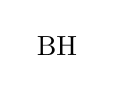
\begin{tikzpicture}
\node at (0,0) {BH};
\end{tikzpicture}
}
\end{center}

																					
\section{Einstein equivalence principle}
We will define this (the weak and strong equivalence principles), and some of the tests been performed.

\subsection{Weak equivalence principle}
Trajectory of body in free fall is independent of its mass and $\underbrace{\text{composition}}_{\text{binding energy}}$ (as per Galileo, feather vs. brick). Note that this is not equivalent for electric fields (the movement of a charged particle through an electric field depends on its charge).

\subsection{Strong equivalence principle}
\begin{enumerate}
\item weak equivalence principle is valid
\item results of any non-gravitational (e.g. EM, \underline{not} Cavendish expt) experiment is independent of velocity of freely falling frame
\begin{itemize}
\item this is \emph{local Lorentz invariance}
\end{itemize}
\item results of non-gravitational experimental are independent of where and when it is performed
\begin{itemize}
\item this is \emph{local position invariance}
\end{itemize}
\end{enumerate}

The Einstein equivalence principle (EEP) $\equiv$ strong implies: existence of a ``curved spacetime'' with:
\begin{enumerate}
\item[\textbf{i.}] symmetric metric
\item[\textbf{ii}.] trajectories of free-falling bodies are geodesics of metric
\item[\textbf{iii.}] the laws of physics in a freely-falling frame can be written in the language of special relativity
\end{enumerate}


\review{
Einstein equivalence principle:
\begin{enumerate}
\item universality of free fall
\item local Lorentz invariance
\item local position invariance
\end{enumerate}
Implications:
\begin{enumerate}
\item[3)] $\Rightarrow$ fundamental constant independent of $\vec{x}$, $t$
\item[2)] $\Rightarrow$ laws of non-gravitational physics \underline{locally} independent of frame
\item[1)] $\Rightarrow$ space is \underline{curved}
\end{enumerate}

Why is space curved? Locally straight trajectory in free yet \underline{yet} gravity produces curved trajectory (observed) $\Rightarrow$ only possible if coordinates change from one point to next
}

\section{Experimental tests}
\subsection{Experimental tests of free fall}
Inertial mass $m_i=\frac{\text{applied non-gravitational force}}{\text{measured acceleration}}$

Gravitational mass $m_g=$ ``passive'' mass appearing in weight

Look for $m_i \neq m_g$

Write 
\begin{equation}
m_g=m_i + \sum_{\text{interactions A in body}}\eta^A \frac{E^A}{c^2}
\end{equation} 
Here $E=$ ``binding energy''/potential energy of interaction $A$.

\underline{Tests:}
\begin{enumerate}
\item E{\"o}tv{\"o}s-type torsion balance experiments: two different materials may fall at difference rates (see Dicke, Braginsky)
\item Colorado: U, Cu laser interferometer $\Rightarrow$ relativite acceleration
\item E{\"o}t-Wash experiments: fancy version of (1)
\end{enumerate}

Result:
\begin{equation}
\frac{|m_g-m_i|}{m_i}\leq 10^{-13}
\end{equation}

We test this, for example, with aluminium (Al) and gold (Au) weights on a torsion balance. As the Sun moves from one side of the Earth to the other, if the gravitational mass of either differs from the other we will see diurnal oscillation in the balance.

\picture{images/eotvos.png}

\subsection{Tests of local Lorentz invariance}
\begin{itemize}
\item Michelson-Morley experiment (the aether)
\item Rossi-Hall tests for lifetime of muons (time dilation $\Leftrightarrow$ LLI)
\item Ives-Stiwell transverse Doppler shift
\begin{itemize}
\item laser travelling some vector $\vec{v}$
\item we see perpendicular wave vector $\vec{k}$
\item measure frequency when laser intersects line of sight
\item Doppler shift arises due to time dilation
\end{itemize}
\end{itemize}

Mathematically:
\begin{equation}
\bmx{\omega'/c\\k'_x\\k'_y\\k'_z}=
\bmx{
\gamma&\gamma v/c&0&0\\
\gamma v/c&\gamma&0&0\\
0&0&1&0\\
0&0&0&1
}
\bmx{
\omega/c\\0\\k_y\\0
}=
\bmx{
\gamma\omega/c\\
\gamma\omega v^2/c\\
k_y\\
0
}
\end{equation}

\exercise{Compare with standard longitudinal Doppler:
\begin{equation}
\pmx{\\\text{same}\\\text{matrix}\\\\}\pmx{\omega/c\\k_x\\0\\0}
\end{equation}
}
{}

\review{Last lecture:
\begin{itemize}
\item tests of LPI
\item Schiff's thought experiment (gravitational redshift)
\end{itemize}
}

\subsection{Gravitational redshift}
\begin{equation}
\frac{h\nu'-h\nu}{h\nu}=\frac{(m_A g_A - m_B g_B)H}{(m_A-m_B)c^2}
\end{equation}
If $g_A=g_B$ (universal free-fall), then gravitational redshift is $gH/c^2$

\subsection{Observation of GR in experiments}
There are situations where GR makes measurable difference \underline{today}

\begin{itemize}
\item Pound-Rebka experiment (gravitational redshift, also seen on white dwarf spectral lines)
\item GPS
\item 2015 discovery of gravitational waves from binary BH merger
\item cosmological measurements (CMB, redshifts, $H_0$, \ldots)
\item gravitational lensing (light bent by a mass) (see: Einstein cross, Abell clusters, stars behind Sun)
\item precession of perihelion of Mercury
\item orbital decay of Hulse-Taylor binary pulsar (can calculate to mm precision the decay of the orbit every 8 hours due to gravitational wave emission)
\item Nordtredt/lunar ranging experiments
\item Gravity Probe B - lense-thinning precession
\item Shapiro time delay
\end{itemize}

\begin{figure}[h]
\centering
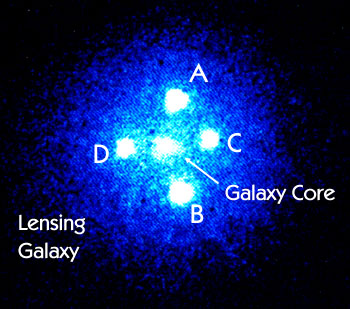
\includegraphics[width=0.5\textwidth]{images/einstein-cross.jpg}
\caption{Einstein cross}
\end{figure}


\subsubsection{Pound-Rebka experiment}
Looks at gravitational redshift of $\SI{14.4}{keV}$ gamma rays from $^{57}$Fe decay

$^{57}$Fe decays and emits photons directly down from a $\SI{23}{m}$ tall tower, to another box of $^{57}$Fe below. Gravitational redshift occurs; time moves slower closer to the Earth, so gamma ray emitted will have a different energy than that required to be absorbed by the $^{57}$Fe at the bottom.

Receiver box moves up/down at speed $v$. We adjust $v$ at bottom so that kinematic Doppler shift $\propto \left(\frac{1-v/c}{1+v/c}\right)^{1/2}$ exactly cancels the gravitational redshift $\propto gH/c^2$

N.B.: recoil (in a random direction) when photon emitted/absorbed; energy $E_R=\frac{E_\gamma}{2M_{Fe}c^2}$

\begin{equation}
E_R\sim\frac{\SI{14.4}{keV}}{\SI{100}{GeV}}\sim 10^{-7}
\end{equation}

We solve this problem through the Mossbauer effect: use whole crystal; whole crystal ($\sim10^{23}$ Fe atoms) recoils

\begin{figure}[h]
\centering
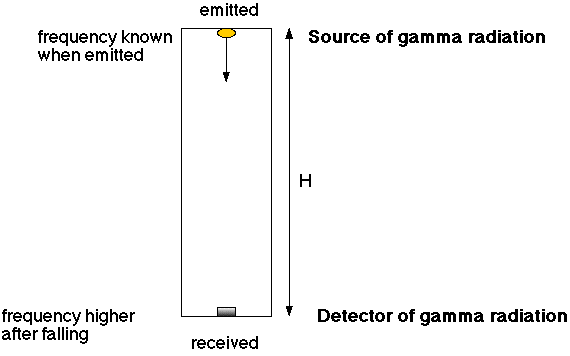
\includegraphics[width=0.5\textwidth]{images/pound-rebka.png}
\caption{Pound-Rebka experiment}
\end{figure}


\subsubsection{Lunar ranging}
Williams + Dickey (2002)\footnote{See also ``Living Reviews'' Relativity}

Moon not completely dormant
\begin{itemize}
\item fluid core (?)
\item tidal dissipation internally
\item etc \ldots
\end{itemize}

Multiple radar reflectors to improve accuracy. We search for an accurate Earth-Moon orbit versus time; we find
\begin{equation}
\frac{1}{G}\frac{dG}{dt}=(0.0\pm 1.1)\times \SI{d-12}{yr^{-1}}
\end{equation}

Uncertainty $\approx 0.02 H_0$ - we don't see increasing separation between Earth and Moon due to expansion of universe. This is expected, however: gravitational bound objects do not separate with time, although the energy they require to stay bound will increase

\subsubsection{Deflection of light (gravitational lensing)}
In a three-body system with the Earth, the Sun and another star, the light from the star will bend due to the Sun before it reaches Earth (not taking a straight path). This causes the apparent position of the star to be different than the actual position.

Deflection angle $\delta\theta \propto \frac{GM}{c^2d}$

GR deflection = $2\times$ Newtonian deflection (Einstein 1911). 

This effect is achromatic!

\subsubsection{Shapiro delay}
Roundtrip time from Earth to a distant mirror (in a three-body system including the Sun) is longer than if the Sun was not there.
\begin{equation}
\delta t\propto \frac{GM}{c^3}\ln(\text{geometric factors})
\end{equation}

Best measurements with Cassinin spacecraft (accuracy 1 in $10^5$)

\section{Geometric Objects}

\subsection{Vectors}
Invariants are measurable. Therefore, each coordinate representation is as valid as the other!

\subsubsection{Definitions of a vector}
Vector $\vec{A}$
\begin{itemize}
\item four numbers that are projections onto spacetime (can be dependent or independent of a metric)
\begin{itemize}
\item Note: vectors can have meaning without a metric
\end{itemize}
\item a geometric object with ``length'' (requires a metric) and a ``direction'', i.e. an arrow
\item a geometric object which transforms from one coordinate system to another
\item a linear function which takes a 1-form as an argument and returns a real number
\end{itemize}

$\underbrace{\text{Vector spaces}}_{\text{vectors}}\supseteq \underbrace{\text{normed vector spaces}}_{\text{length}} \supseteq \underbrace{\text{inner product spaces}}_{\text{angle}}$

$\Rightarrow$ you can have vector spaces without a norm or angle concept.

\exercise{$\vec{\Delta}x=$ displacement (in spacetime), is a vector}{}

Vector components, $A^0,A^1,A^2,A^3$; in another frame we have $A^{0'},A^{1'},A^{2'},A^{3'}$.

\subsubsection{What is a basis vector?}
Projection requires a metric (for a dot product)!
$\Rightarrow$ we have 4, special, linearly independent vectors which ``point along'' (no concept of length/angle) axes of coordinate system, $\left\{\vec{e}_{\alpha}\right\}$

\begin{equation}
\vec{A}=A^0 \vec{e}_{0} +A^{1}\vec{e}_{1}+A^{2}\vec{e}_{2}+A^{3}\vec{e}_{3} \label{vector projection}
\end{equation}

As $\vec{e}_{0}$ is itself a vector, using \ref{vector projection}
\begin{equation}
\vec{e}_{0}=(\vec{e}_{0})^{0}\vec{e}_{0}+(\vec{e}_{0})^{1}\vec{e}_{1}+(\vec{e}_{0})^{2}\vec{e}_{2}
+\underbrace{(\vec{e}_{0})^{3}}_{\mathclap{\text{3rd component of }\vec{e}_{0}}}\vec{e}_{3}
\end{equation}

By linear independence, as $\vec{e}_0$ is linearly independent to $\vec{e}_{1},\vec{e}_{2},\vec{e}_{3}$
\begin{equation}
\Rightarrow (\vec{e}_{0})^{1}=(\vec{e}_{0})^{2}=(\vec{e}_{0})^{3}=0
\end{equation}
\begin{equation}
\Rightarrow (\vec{e}_{\alpha})^{\beta}=\delta_{\alpha}^{\beta}
\end{equation}
which is \emph{true in all coordinate systems}. Therefore in a primed frame,
\begin{equation}
\Rightarrow (\vec{e}_{\alpha'})^{\beta'}=\delta_{\alpha'}^{\beta'}
\end{equation}

\underline{But} $(\vec{e}_{\alpha'})^{\beta}\neq \delta^{\beta}_{\alpha'}$
\begin{itemize}
\item $\vec{e}_{\alpha'}$ is tied to the prime frame
\item the geometric object is only defined with respect to the frame (where $\vec{A}$ could exist in all frames)
\item you cannot measure a basis vector in another coordinate frame. You have to be in the coordinate frame to measure it.
\end{itemize}

\subsubsection{Transformations}
In general,
\begin{align*}
\left\{x^{\beta'}\right\}&\mapsto \left\{x^{\alpha}\right\}\\
\text{from }\sigma' &\to \sigma\quad\text{primed to unprimed}
\end{align*}

\begin{equation}
\Lambda^{\alpha}_{\beta'}=\frac{\partial (x^{0},x^{1},x^{2},x^{3})}{\partial (x^{0'},x^{1'},x^{2'},x^{3'})}
=\frac{\partial x^{\alpha}}{\partial x^{\beta'}}\quad \text{16 elements!}
\end{equation}

If the transform is linear (e.g. Lorentz transform), we can consider
\begin{equation}
x^{\alpha}=\Lambda^{\alpha}_{\beta'}x^{\beta'}
\end{equation}
where $\Lambda^{\alpha}$ is not necessarily a constant. But if the transform is non-linear, the left side is wrong. We instead have
\begin{equation}
dx^{\alpha}=\Lambda^{\alpha}_{\beta'}~dx^{\beta'}
\end{equation}

Why? If we define $\vec{x}$ as a displacement from origin to the point in a curved space, there are multiple different path. We would need more than 4 numbers to define this, therefore we no longer have a meaningful vector. 

Vectors are defined locally in tangent space, \textbf{and} transformations of vectors are also restricted locally to tangent space. If $\vec{A}$ is a vector,
\begin{equation}
A^{\alpha}=\Lambda^{\alpha}_{\beta'}A^{\beta'}
\end{equation}

\review{\textbf{Vectors}

$\vec{A}$: defined in tangent space

Components $A^\alpha$: $\vec{A}=A^\alpha \vec{e}_{\alpha}$ where $\vec{e}_{\alpha}$ are basis vectors. These (unprimed) basis vectors only have meaning in unprimed coordinates

Transform like infinitesimal displacements:
\begin{equation}
\underbrace{A^{\alpha'}}_{\text{primed}}=\overbrace{\frac{\partial x^{\alpha'}}{\partial x^{\alpha}}}^{\mathclap{\text{transform matrix}}}\underbrace{A^{\alpha}}_{\text{unprimed}}\label{vector transform}
\end{equation}

How do basis vectors transform?
\begin{align*}
A^{\alpha}\vec{e}_\alpha=\vec{A}&=A^{\alpha'}\vec{e}_{\alpha'}\\
&=\frac{\partial x^{\alpha'}}{\partial x^{\beta}}A^{\beta}\vec{e}_{\alpha'}	\\
&=\frac{\partial x^{\alpha'}}{\partial x^{\alpha}}A^{\alpha}\vec{e}_{\alpha'}
\end{align*}

This has to be true for all $\vec{A}$, i.e.
\begin{equation}
\vec{e}_{\alpha}=\frac{\partial x^{\alpha'}}{\partial x^{\alpha}}\vec{e}_{\alpha'}
\end{equation}
Or equivalently,
\begin{equation}
\vec{e}_{\alpha'}=\frac{\partial x^{\alpha}}{\partial x^{\alpha'}}\vec{e}_{\alpha}
\end{equation}
Note this is the opposite of transformation law for vector components \ref{vector transform}

\exercise{Try for Lorentz transformations.}{}
\exercise{(later) Try for 2 types of Schwarz black hole coordinates.}{}

\example{}{
Lorentz transformation: frame $\bar{\mathcal{O}}$ moving with speed $v$ in the $x$-direction as seen from frame $\mathcal{O}$

\begin{equation}
\frac{\partial x^{\bar{\beta}}}{\partial x^{\alpha}}=\pmx{\gamma&-\gamma v&0&0\\
-\gamma v&\gamma & 0&0\\ 0&0&1&0\\0&0&0&1}
\end{equation}
Consider vector $\vec{A}=(5,0,0,2)$ in $\mathcal{O}$, i.e.
\begin{equation}
\vec{A}=5\vec{e}_0 + 2\vec{e}_3
\end{equation}

What is $A^{\bar{0}}$?
\begin{align}
A^{\bar{0}}&=\frac{\partial x^{\bar{0}}}{\partial x^0}A^0 + \frac{\partial x^{\bar{0}}}{\partial x^1}A^1
+\frac{\partial x^{\bar{0}}}{\partial x^2}A^2 + \frac{\partial x^{\bar{0}}}{\partial x^3}A^3\\
&=\gamma A^0 - \gamma v\cdot 0 + 0\cdot 0 + 0\cdot 2\\
&=5\gamma\\
\text{Similarly, }A^{\bar{1}}&=-5\gamma v\\
A^{\bar{2}}&=0\\
A^{\bar{3}}&=2
\end{align}

Now determining the basis vectors for $\bar{O}$,
\begin{align}
\vec{e}_{\bar{\alpha}}&=\Lambda^{\alpha}_{\ph{\alpha}\bar{\alpha}}(-v)\vec{e}_{\alpha}
\intertext{Note since we are taking the inverse Lorentz transform, we replace $v$ by $-v$.}
&=\frac{\partial x^0}{\partial x^{\bar{0}}}\vec{e}_0 + \frac{\partial x^1}{\partial x^{\bar{0}}}\vec{e}_1
+\frac{\partial x^2}{\partial x^{\bar{0}}}\vec{e}_2 + \frac{\partial x^3}{\partial x^{\bar{0}}}\vec{e}_3\\
&=\gamma \vec{e}_0 + \gamma v \vec{e}_1\\
\vec{e}_{\bar{1}}&=\gamma v \vec{e}_0 + \gamma \vec{e}_1\\
\vec{e}_{\bar{2}}&=\vec{e}_2\\
\vec{e}_{\bar{3}}&=\vec{e}_3
\end{align}
Likewise, we can determine the basis vectors for $\mathcal{O}$ in terms of $\bar{\mathcal{O}}$'s basis vectors,
\begin{align}
\vec{e}_0&=\gamma \vec{e}_{\bar{0}}-\gamma v \vec{e}_{\bar{1}}\\
\vec{e}_1 &= -\gamma v \vec{e}_{\bar{0}}+\gamma \vec{e}_{\bar{1}}
\end{align}
}

}

\subsection{1-forms}
$\widetilde{p}$
\begin{itemize}
\item four numbers associated to four dimensions and associated to vectors in a specific way (see below)
\item geometric object that transforms like a \underline{gradient}
\item tensor of type $\pmx{0\\1}$, i.e. linear function which accepts vector as an argument and returns a real number
\end{itemize}
If we have a metric, a neat way to visualise a 1-form is as a contour.

e.g. vector is an arrow (length, direction)

cf. 1-form is contours

\picturesize{images/contour.png}{0.3}
Value of $\widetilde{p}(\vec{A})=4$; number of times $\vec{A}$ pierces surfaces of $\widetilde{p}$

Components defined to be
\begin{align*}
p_\alpha&=\widetilde{p}(\vec{e}_{\alpha})\\
&=\langle{\tilde{p},\vec{e}_{\alpha}}\rangle
\end{align*}
From lines 1 to 2, we have equivalent notation. We are using an inner product. By convention we use a lowered index.

We cannot have curved contours, as they are only defined in tangent space.

We have a neat way to calculate the coordinate-independent quantity $\tilde{p}(\vec{A})$
\begin{align*}
\tilde{p}(\vec{A})&=\tilde{p}(A^{\alpha}\vec{e}_{\alpha})\\
&=A^{\alpha}\tilde{p}(\vec{e}_{\alpha})\quad\text{linear}\\
&=A^{\alpha}p_{\alpha}
\end{align*}

This is a contraction. It is an inner product but \underline{not} dot product (we require a metric, and for it to be between two vectors, for a dot product).

Vectors and 1-forms are ``apples and oranges'' - completely different geometric objects which cannot be compared even at the same point, e.g. $\tilde{p}=\vec{A}$ is meaningless.

This is comparable to bras and kets in quantum mechanics; they form a dual space, but we cannot directly compare the objects of a pair

\subsubsection{How do 1-forms transform?}
We start with basis vectors
\begin{equation}
\vec{e}_{\alpha}=\frac{\partial x^{\alpha'}}{\partial x^{\alpha}}\vec{e}_{\alpha'}
\end{equation}
In component form:
\begin{align*}
p_{\alpha'}&=\tilde{p}(\vec{e}_{\alpha'})\\
&=\frac{\partial x^{\alpha}}{\partial x^{\alpha'}}\tilde{p}(\vec{e}_{\alpha})\quad\text{linear}\\
&=\frac{\partial x^{\alpha}}{\partial x^{\alpha'}}p_{\alpha}
\end{align*}
i.e. components of $\tilde{p}$ transform like basis vectors (\underline{not} components of basis vectors)

We can now prove that contraction is independent of coordinates.
\begin{align}
<\tilde{p},\vec{A}>&=p_{\alpha'}A^{\alpha'},\quad\text{components in primed coordinates}\\
&=\frac{\partial x^{\alpha}}{\partial x^{\alpha'}}p_{\alpha}\frac{\partial x^{\alpha'}}{\partial x^{\beta}A^{\beta}}
\intertext{noting $\frac{\partial x^{\alpha}}{\partial x^{\alpha'}}\times \frac{\partial x^{\alpha'}}{\partial x^{\beta}A^{\beta}}=\delta^{\alpha}_{\ph{\alpha}\beta}$; it is the transform matrix $\Lambda^{\alpha}_{\ph{\alpha}\alpha'}$ multiplied by its inverse.}
&=p_{\alpha}A^{\alpha}
\end{align}
i.e. the inner product is the same in both coordinates!

\subsection{1-forms, basis 1-forms and gradients}



Given components of a 1-form $p_0,p_1,p_2,p_3$, how do we recreate the geometric object $\tilde{p}$?

Naively, we could say
\begin{equation*}
\tilde{p}=p_0\vec{e}_0 + p_1 \vec{e}_1 + p_2\vec{e}_2 + p_3\vec{e}_3
\end{equation*}This is \underline{wrong}. ``All indices down.... bad''. A 1-form is not a vector (so we cannot simply construct them from basis vectors)!

We need 1-form basis $\tilde{\omega}^0, \tilde{\omega}^1, \tilde{\omega}^2, \tilde{\omega}^3$. We write
\begin{equation}
\tilde{p}=p_{\alpha}\tilde{\omega}^\alpha
\end{equation}

How do we construct the 1-form basis? Use contraction which relates objects in the dual space. Take any $\tilde{p},\vec{A}$,
\begin{align}
p_{\alpha}A^\alpha &\langle \tilde{p},\vec{A} \rangle\\
&=\langle p_{\beta}\tilde{\omega}^\beta,A^\gamma \vec{e}_\gamma \rangle\\
&=p_\beta A^\gamma \langle \tilde{\omega}^\beta,\vec{e}_\gamma \rangle
\end{align}
which is true for any $\tilde{p},\vec{A}$. Obviously this is only possible if
\begin{equation}
\langle \tilde{\omega}^\beta,\vec{e}_\gamma \rangle=\delta^{\beta}_{\ph{\beta}\gamma}
\end{equation}

If $e$'s have 1,0 inside, so do $\omega$'s, e.g. $\tilde{\omega}^2 = (0,0,1,0)$.

\exercise{Show that 1-form bases transform as
\begin{equation}
\tilde{\omega}^{\alpha'}=\frac{\partial x^{\alpha'}}{\partial x^{\alpha}}\tilde{\omega}^{\alpha}
\end{equation}
i.e. basis 1-forms transform just like vectors.}
{}

\begin{table}[h]
\centering
\begin{tabular}{l  | c | c}
\renewcommand\arraystretch{1}
& \textbf{Vectors} & \textbf{1-forms}\\
\renewcommand\arraystretch{2}
& $\vec{A}=A^{\alpha}\vec{e}_{\alpha}$&$p_{\alpha}=\tilde{p}(\vec{e}_{\alpha})$\\
\hline Transformation for coordinates & 
$A^{\alpha'}=\dfrac{\partial x^{\alpha'}}{\partial x^{\alpha}}A^{\alpha}$ &
$p_{\alpha'}=\dfrac{\partial x_{\alpha'}}{\partial x_{\alpha}}p_{\alpha}$ \\
\hline Transformation for basis vectors &
$\vec{e}_{\alpha'}=\dfrac{\partial x_{\alpha'}}{\partial x_{\alpha}}\vec{e}_{\alpha}$ &
$\tilde{\omega}^{\alpha'}=\dfrac{\partial x^{\alpha'}}{\partial x^{\alpha}}\tilde{\omega}^{\alpha}$
\end{tabular}
\end{table}

\subsection{Gradiants}

The spacetime derivatives of a sclar function (i.e. $\frac{\partial \phi}{\partial x^\alpha}$ form a 1-form, e.g. frequency and wavenumber make a 1-form. This is because:
\begin{itemize}
\item if we combine with $\vec{x}=(t,\vect{x})$ then we get the number of peaks and troughs in waves
\item (equivalently) frequency $=\frac{\partial}{\partial t}$(phase), wavenumber $=\nabla($phase) ($\nabla$ is the 3D gradient)
\end{itemize}

Consider a particle moving on a worldline $\vec{x}(\tau)$, where $\tau$ is the \emph{proper time}. Consider also a scalar filed $\phi(\vec{x})$. How does a particle see $\phi$ changing on its worldline?

\begin{equation}
\underbrace{\frac{d\phi}{d\tau}}_{\mathclap{\text{number}}}
=\frac{\partial \phi}{\partial x^\alpha}\underbrace{\frac{dx^\alpha}{d\tau}}_{\mathclap{\text{vector 4-velocity}}},
\quad\text{chain rule}
\end{equation}
i.e. $\frac{\partial \phi}{\partial x^{\alpha}}$ must be a 1-form. Notation: $\tilde{d\phi}$ is a geometric object, $\frac{\partial \phi}{\partial x^\alpha}$ is its components.


\review{Given a scalar field $\phi(\vec{x})$ we define a 1-form $\tilde{d\phi}$, with components $(\tilde{d\phi})_{\alpha}=\frac{\partial\phi}{\partial x^{\alpha}}$

\textbf{Notes:}
\begin{enumerate}
\item If we take $\phi$ = one of the coordinates, e.g. $\phi=x^{\alpha}$ for a specific $\alpha$, then $\tilde{d\phi}=\delta^{\alpha}_{\beta}$ for $\phi=x^{\alpha}$
\begin{itemize}
\item i.e. $\tilde{d \phi}$, for $\phi=x^{\alpha}$ is just $\tilde{\omega}^{\alpha}$, the basis 1-form
\end{itemize}
\item $\tilde{d\phi}$ is the most natural definition of a normal in GR. We also has $\tilde{d\phi}(\vec{t})=0$ if $\vec{t}$ is a tangent vector to the level surfaces of $\phi$; don't need a metric
\item How do we construct components of vectors?
\begin{itemize}
\item Components of 1-forms: $p_{\alpha}=\tilde{p}(\vec{e}_{\alpha})$
\item Dual: components of vectors: $A^{\alpha}=\vec{A}(\tilde{\omega}^{\alpha})$
\item Note that we do not need 1-forms to define vectors (and vice versa), but once we start discussing components, we do need them
\end{itemize}
\end{enumerate}
}

\subsection{Tensors}
$\pmx{M\\N}$ tensor is a linear function operating on M 1-forms and N vectors to return a real number. 

For example if $R$ is a $\pmx{1\\1}$ tensor then its components are $R^{\alpha}_{\beta}=R(\tilde{\omega}^{\alpha},\vec{e}_{\beta})$.

You can build big tensors out of little ones in several ways (and vice versa, e.g. via contraction). One important way is the outer product; 

e.g. outer product of vectors $\vec{A}$ and $\vec{B}=\pmx{2\\0}$ tensor; $T=\vec{A}\otimes \vec{B}$

Takes two 1-forms as arguments: $T(\tilde{p},\tilde{q}) \equiv^{\text{def}}\vec{A}(\tilde{p})\vec{B}(\tilde{q})$ (this is multiplying two scalar numbers)

\begin{itemize}
\item Note: outer product not commutative.
\begin{equation}
\text{If } S=\vec{B}\otimes \vec{A} \text{ then } S(\tilde{p},\tilde{q})=\vec{B}(\tilde{p})\vec{A}(\tilde{q})\neq T(\tilde{p},\tilde{q})
\end{equation}
\item Can't write a general $\pmx{M\\N}$ tensor as an outer product necessarily, but can write as a linear combination of outer products
\begin{equation}
\underbrace{T}_{\mathclap{\text{geometric object}}}=T^{\alpha_{1},\ldots,\alpha_{M}}_{\beta_{1},\ldots,\beta_{N}}\vec{e}_{\alpha_{1}}\otimes\ldots\otimes \vec{e}_{\alpha_{M}}\otimes \tilde{\omega}^{\beta_{1}}\otimes\ldots\otimes\tilde{\omega}^{\beta_{N}}
\end{equation}
\item even though we use M 1-forms and N vectors, we take the outer product over N 1-forms and M vectors
\end{itemize}

\exercise{Show that you get the components of $T$ when you evaluate $T$ for $M$ basis 1-forms and $N$ basis vectors.}{}

Another way to generate new tensors:
\begin{align*}
\text{Symmetric part of T ($T^{(\alpha\beta)}$): }& T_{\text{(sym)}}^{(\tilde{p},\tilde{q})}=\frac{1}{2}T(\tilde{p},\tilde{q})+\frac{1}{2}T(\tilde{q},\tilde{p})\\
\text{Antisymmetric part of T ($T^{[\alpha\beta]}$): }& T_{\text{(sym)}}^{(\tilde{p},\tilde{q})}=\frac{1}{2}T(\tilde{p},\tilde{q})-\frac{1}{2}T(\tilde{q},\tilde{p})\\
\end{align*}

This example is for $\pmx{2\\0}$ but can generalise to $\pmx{M\\N}$

\subsubsection{Metric tensor}
$\pmx{0\\2}$ tensor which accepts two vectors and returns a number which we call scalar or dot product.

\begin{equation}
g(\vec{A},\vec{B})\equiv^{def}\vec{A}\cdot \vec{B}\qquad\text{this is \underline{not} contraction}
\end{equation}

Clearly bilinear

What is g? Anything we like! It depends on the coordinates we choose to use! (And it tells us how lengths, angles, $\ldots$ are measured in our favourite coordinates)

Components: 
\begin{equation}
g_{\alpha\beta}=g(\vec{e}_{\alpha},\vec{e}_{\beta})=\vec{e}_{\alpha}\cdot \vec{e}_{\beta}
\end{equation}
i.e. 16 numbers saying how the basis vectors relate to each other in any given coordinate system

What is $g(\Delta\vec{x},\Delta\vec{x})$ ($\Delta\vec{x}$ is a displacement vector)?
\begin{align*}
g(\Delta\vec{x},\Delta\vec{x})&=g(\Delta x^{\alpha}\vec{e}_{\alpha},\Delta x^{\beta}\vec{e}_{\beta})\\
&=g_{\alpha\beta}\Delta x^{\alpha}\Delta x^{\beta} \qquad\text{linear}
\end{align*}

This quantity is the spacetime interval in curved space. Invariant!

\review{Metric: $\pmx{0\\2}$ tensor $g(\vec{A},\vec{B}\equiv \vec{A}\cdot\vec{B}$

Components: 
\begin{equation}
g_{\alpha\beta}=g(\vec{e}_{\alpha},\vec{e}_{\beta})=\vec{e}_{\alpha}\cdot \vec{e}_{\beta}
\end{equation}
}

e.g. Minkowski metric
\begin{equation}
\{g_{\alpha\beta}\}=\text{diag}(-1,1,1,1)
\end{equation}
e.g. Schwarzschild black hole of mass $M$ (we will prove this later)
\thinmuskip=5mu
\begin{equation}
\{g_{\alpha\beta}\}=\left[-\left(1-\frac{2M}{r}\right),\left(1-\frac{2M}{r}\right)^{-1},~r^2,~r^2\sin^2\theta\right]
\end{equation}
where $r$ is the radial coordinate.

Vectors $\vec{A}$ and $\vec{B}$ are orthogonal vectors if $g(\vec{A},\vec{B})=0$. But orthogonal doesn't necessarily mean perpendicular.

These include 4D vectors of ``zero length'':
\begin{itemize}
\item in Minkowski, momentum of photon $\vec{p}=\left(\frac{E}{c},\utilde{p}\right)$ in flat space,
and we know $E=|\underbar{p}|c$ so $g(\vec{p},\vec{p})=-\frac{E^2}{c^2}+|\underbar{p}|^2=0$.
\begin{itemize}
\item i.e. $\vec{p}$ is orthogonal with itself; has zero ``length'' but obviously \underline{not} a zero vector, nor is it perpendicular to itself
\end{itemize}
\item in Minkowski: boost between frames
\picturesize{images/minkowski_boost.png}{0.4}
\begin{itemize}
\item the boost vectors are not perpendicular, but we still have $\vec{e}_{0'}\cdot\vec{e}_{1'}=0$
\end{itemize}
\end{itemize}


\subsection{Correspondence between vectors and 1-forms}

Let $g$ be a metric, and let $\vec{V}$ be an arbitrary vector. Then $g(\vec{V},...)$ has one argument free, and that argument is a vector, so $g(\vec{V},...)$ must be a 1-form. We call it $\tilde{V}$ because it's the 1-form associated with $\vec{V}$. What are its components?

\begin{align*}
V_{\alpha}\equiv^{def}\tilde{V}(\vec{e}_{\alpha})&=g(\vec{V},\vec{e}_{\alpha})\\
&=g(V^{\beta}\vec{e}_{\beta},\vec{e}_{\alpha})\\
&=V^{\beta}g(\vec{e}_{\beta},\vec{e}_{\alpha})\quad\text{by linearity}\\
&=V^{\beta}g_{\beta\alpha}\quad\text{by definition}
\end{align*}
This is the ``lowering the index'' operation of yesteryear! The old language for this is: lower a contravariant index, get a covariant index.

This can go the other way as long as $g$ is invertible. \underline{Define} $g^{\alpha\beta}$ as 16 numbers you get if you treat $g_{\alpha\beta}$ as a matrix and invert it.
\begin{equation}
\text{i.e.,}\quad g^{\alpha\beta}g_{\beta\gamma}=\delta^{\alpha}_{\gamma}
\end{equation}

\exercise{What is the geometric object whose components are $g^{\alpha\beta}$? Hint: $\pmx{2\\0}$ tensor which takes two 1-forms as arguments.}{}

We check that ``raising the index'' on $V_{\alpha}$ gets us back to $\vec{V}$.
\begin{equation}
V_{\alpha}\underbrace{g^{\alpha\gamma}}_{\text{inverse metric}}=
V^{\beta}g_{\beta\alpha}g^{\alpha\beta}=V^{\beta}\delta_{\beta}^{\gamma}
=V^{\gamma}
\end{equation}

More generally:
\begin{align*}
g&\text{ maps } \pmx{M\\N}\text{ tensor to }\pmx{M-1\\N+1}\text{ tensor}\\
g^{-1}&\text{ maps } \pmx{M\\N}\text{ tensor to }\pmx{M+1\\N-1}\text{ tensor}
\end{align*}

Physics example: consider a photon in curved (Schwarzschild) spacetime. 

We know $\vec{p}\cdot\vec{p}=0$ in the local freely falling frame(from weeks 1,2: Michelson-Morley experiment), and $\vec{p}\cdot\vec{p}$ is invariant $\Rightarrow \vec{p}\cdot\vec{p}=0$ in all coordinate systems. 

In Schwarzschild spacetime: radially in-falling photon $\vec{p}=\left(p^0,p^r,0,0\right)$

\begin{align*}
0&=g_{00}(p^0)^2+g_{11}(p^1)^2\\
&=-\left(1-\frac{2M}{r}\right)(p^0)^2+\left(1-\frac{2M}{r}\right)^{-1}(p^r)^2
\end{align*}
i.e.
\begin{align*}
\frac{p^r}{p^0}=\left(1-\frac{2M}{r}\right)^{-1}&\neq 1\\
(\text{phase speed of light})^{-1}&\neq 1
\end{align*}


\section{Kinematics}
In general, for kinematics we do not care about the origin of the force, and only analyse the motion of the object. This is in contrast to dynamics, where we investigate where a force originates. In a GR context, for kinematics this means that we will look into the motion of an object while considering the spacetime, while for dynamics we also investigate what causes the curvature of spacetime.

Event: $\vec{x}=(t,x,y,z)$

Spacetime interval between 2 events: $ds^2=g(d\vec{x},d\vec{x})$

e.g. Minkowski

\picture{images/lightcone.png}

\begin{align}
ds^2=0\qquad &\text{null ray; defines light cone which joins events A and B}\\
ds^2>0\qquad &\text{events A and B and mutually spacelike; can't event get from A to B;}\\
\qquad&\text{there always exists an inertial frame such that events occur at}\nonumber\\
\qquad&\text{different spacial locations at the same time}\nonumber\\
ds^2<0 \qquad& \text{events are timelike; can get from A to B;}\\
\qquad &\text{frame exists where events occur at same spatial location at different times}\nonumber
\end{align}

For $ds^2>0$, we will always be able to Lorentz transform into a frame where two events occur at the same time, but spatially separated. For $ds^2<0$, there will always be a Lorentz transform such that the two events occur at the same spatial location, but temporally separated.

Proper time: two events A and B separated infinitesimally along some 4D trajectory.
\begin{equation}
d\tau \equiv^{def}(-ds^2)^{1/2}
\end{equation}

\picture{images/propertime_path}


$\tau$ is an affine parameter (= label of path) with a particular normalisation, namely that $\tau$ tracks passage of time for an observer at rest with respect to the sequence of events defined by $\vec{x}(\tau)$.

\subsection{4-velocity}

From above:
\begin{align*}
-d\tau^2=ds^2&=d\vec{x}\cdot d\vec{x}\\
\Rightarrow -1&=\frac{d\vec{x}}{d\tau}\frac{d\vec{x}}{d\tau}
\end{align*}
where the dot product is with respect to the metric. 

Call $\vec{u}=\dfrac{d\vec{x}}{d\tau}$ the 4-velocity. It is timelike, and $\vec{x}\propto d\vec{x}$. It relies on a geometric object (the sequence of events $\vec{x}(\tau)$) for its meaning. And if $\tau$ is the label, we have $\vec{u}\cdot \vec{u}=-1$ as normalisation.

\subsubsection{Example 1: Momentarily comoving reference frame}
For example, consider the momentarily comoving reference frame.

\begin{equation}
\frac{d\mathbf{x}}{dt}=0 \qquad \therefore \vec{u}=(u^t,0,0,0)
\end{equation}

By definition $u^t=\frac{dt}{d\tau}$. But what is it? Normalisation gives
\begin{align*}
-1&=g_{tt}(u^t)^2+0\\
u^t&=\left(-\frac{1}{g_{tt}}\right)^{1/2}
\end{align*}

In flat space, $g_{tt}=-1$ and $u^t=1$.

In Schwarzschild space, $g_{tt}=-\left(1-\frac{2M}{r}\right)$ and $u^t=\left(1-\frac{2M}{r}\right)^{-1/2}$. Recall that $u^t \equiv \frac{dt}{d\tau}$. So as $r\to 2M, \frac{dt}{d\tau}\to \infty$. Physically, this says that time slows down as we approach a black hole. $d\tau$ would be the clock nearby the black hole, while $dt$ would be the clock on a faraway observer. They see an infinite amount of ticks on their clock, before the black hole clock ticks even once.

\subsubsection{Example 2}
Consider coordinates in which our body moves with speed $\vect{V}=\frac{d\vect{x}}{dt}$ (in, for example, the x-direction).

\begin{align*}
\vec{u}&=\left(\frac{dt}{d\tau},\frac{dx}{d\tau},0,0 \right)\\
&=\left(\frac{dt}{d\tau}, V\frac{dt}{d\tau},0,0\right) \quad \text{chain rule}
\end{align*}
By normalisation,
\begin{equation}
-1=\vec{u}\cdot\vec{u}=g_{tt}\left(\frac{dt}{d\tau}\right)^2+g_{tx}\left(\frac{dt}{d\tau}\right)^2 V+g_{xx}V^2\left(\frac{dt}{d\tau}\right)^2
\end{equation}

Special cases (note $c=1$):
\begin{align*}
\text{(a) Minkowski:}\quad& g_{tt}=-1\quad g_{tx}=0\quad g_{xx}=1\\
&\therefore -1=-\left(\frac{dt}{d\tau}\right)^2+V^2\left(\frac{dt}{d\tau}\right)^2\\
&\therefore \frac{dt}{d\tau}=\frac{1}{\sqrt{1-V^2}}\\
&\text{and }\vec{u}=\left(\frac{1}{\sqrt{1-V^2}},\frac{V}{\sqrt{1-V^2}},0,0\right)
\end{align*}

\begin{align*}
\text{(b) Schwarz BH:}\quad &g_{tt}=-\left(1-\frac{2M}{r}\right)\qquad g_{tr}=0\qquad g_{rr}=\frac{1}{1-\frac{2M}{r}}\\
&\therefore -1= -\left(1-\frac{2M}{r}\right)\left(\frac{dt}{d\tau}\right)^2+\frac{1}{1-\frac{2M}{r}}V^2 \cdot\left(\frac{dt}{d\tau}\right)^2
\end{align*}

Solve for $\dfrac{dt}{d\tau}$ again.

N.B. Self-consistently combines time dilation due to gravity (e.g. Pound-Rebka experiment) and motion (e.g. special relativity). It is \underline{not} a simple addition!


\review{Last lecture: kinematics; $\vec{u}$ and time dilation}


\subsection{Energy measurements}

Suppose an observer with 4-velocity $\vec{u}$ encounters a particle with 4-momentum $\vec{p}$. What is the energy $E$ of the particle measured by the observer? (Note: $\vec{u}$ and $\vec{p}$ are geometric objects - they can be considered without reference to a frame (frame-independent). However, the energy measured by the observer is a frame-dependent quantity)

\textbf{Equivalence principle}: we can always ``jump'' into a \emph{freely falling} frame at the location of the particle. In that frame, spacetime is flat $\Rightarrow$ we can describe the frame in Minkowski coordinates. 

\textbf{Local Lorentz invariance}: we can boost ourselves so that we are instantaneously at rest with respect to the particle.

We now know:
\begin{align*}
g&=(-1,1,1,1)\\
\vec{v}&=(1,0,0,0)\\
\vec{p}&=(E,p^x,p^y,p^z)\quad \text{from special relativity}
\end{align*}

Can we express $E$ as an invariant? Yes!
\begin{equation}
E=-\vec{u}\cdot\vec{p},
\end{equation}
recalling the dot product
\begin{equation}
\vec{u}\cdot\vec{p}=g_{\alpha\beta}u^{\alpha}p^{\beta}.
\end{equation}


This is invariant, meaning it is independent of coordinates. We can always use this result even when we're given $\vec{u}$ and $\vec{p}$ in some other coordinates (from the principle of equivalence).

\example{?}{Consider a Schwarz. BH with coordinates $(t,r,\theta,\phi)$. Consider a radially infalling observer at some speed $V$, at some radius $r$. Then $\vec{u}=(u^t,Vu^t,0,0)$ and normalisation $\vec{u}\cdot\vec{u}=-1$ tells us $u^t$ given the metric $g_{tt}=-(\left(1-\frac{2M}{r}\right)$, $g_{rr}=\left(1-\frac{2M}{r}\right)^{-1}$. We dot product with $\vec{p}$ to get $E$.}

\exercise{Measure velocity $V$ as well as energy $E$, and package into a 4-vector with the form\footnote{See Misner, Thorne and Wheeler, exercise 2.5}
\begin{equation}
\vec{V}=\frac{\vec{p}+(\vec{p}\cdot\vec{u})\vec{u}}{-\vec{p}\cdot\vec{u}}
\end{equation}
}{}

\exercise{What is the Doppler shift measured by a stationary observer who shines a laser at a moving mirror at speed $V$ and measures reflected light?
}{}
\begin{figure}[h]
\centering
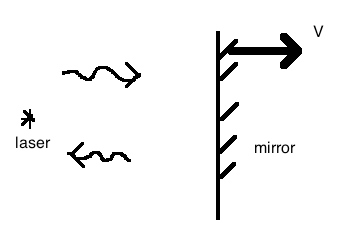
\includegraphics[width=0.35\textwidth]{images/mirror.png}
\caption{Mirror}
\end{figure}

\subsection{4-acceleration}
The definition $\vec{u}=\frac{d\vec{x}}{d\tau}$ is completely general in curved space. But acceleration is \underline{not} $\vec{a}=\frac{d\vec{u}}{d\tau}$ in general. This is because the 2nd derivative $\frac{d^2\vec{x}}{d\tau^2}$ cares about curvature (while the 1st derivative does not).

Actually: $\vec{a}=\nabla_{\vec{u}}\vec{u}$ in general.

In flat space: $\vec{a}=\frac{d\vec{u}}{d\tau}$, which is a special case.

\begin{equation}
\underbrace{\vec{u}\cdot\vec{u}=-1}_{\text{normalisation}}\Rightarrow \underbrace{\vec{u}\cdot\vec{a}=0}_{\text{differentiate both sides w.r.t $\tau$}}\label{4-accel diff}
\end{equation}
Equation (\ref{4-accel diff}) is true in curved space.

\hrule

Let's consider a case of \textbf{Uniform acceleration}. Consider a rocket ship with constant \emph{proper} acceleration $g$ in the ``1'' direction (achieved by, for example, throwing bricks out the back of the rocket at a constant rate), in flat spacetime.

In momentarily comoving reference frame:
\begin{align*}
g&=(-1,1,1,1)\\
\vec{u}&=(1,0,0,0)\\
\vec{a}&=(0,\frac{d^2\vec{x}}{d\tau^2},0,0)
\end{align*}
Above, $a^0$ is zero because
\begin{equation}
-a^t=\vec{u}\cdot\vec{a}=0
\end{equation}
and $a^1$ is equal to $g$ by definition. Hence $\vec{a}\cdot\vec{a}=g^2$. This invariant $\Rightarrow$ true in all coordinates, but ONLY true in \emph{flat spacetime}.

Now consider motion in global Minkowski coordinates not tied to the rocket (which exists because spacetime is flat).

We want to solve for $u^0(\tau),u^1(\tau),a^0(\tau),a^1(\tau)$ in general.
\begin{align*}
\vec{u}\cdot\vec{u}&=-1&-(u^0)^2+(u^1)^2&=-1\\
\vec{a}\cdot\vec{u}&=0& -a^0 u^0+u^1 a^1&=0 \\
\vec{a}\cdot\vec{a}&=g^2& -(a^0)^2+(a^1)^2&=g^2
\end{align*}
Eliminating variables and solving (using straightforward algebra), we obtain 
\begin{align}
\frac{du^0}{d\tau}&=a^0=gu^1\\
\frac{du^1}{d\tau}&=a^1=gu^0
\end{align}
Integrating these gives
\begin{align}
t&=\frac{1}{g}\sinh g\tau\\
x&=\frac{1}{g}\cosh g\tau
\end{align}

\begin{figure}[h]
\centering
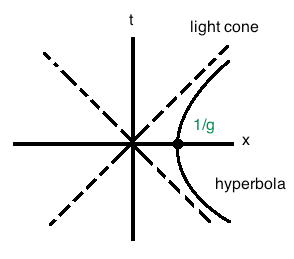
\includegraphics[width=0.3\textwidth]{images/rocket_hyperbola.png}
\caption{Rocket hyperbola}
\end{figure}

Remember this is in \emph{flat spacetime} The interesting thing about this diagram is that is shows that ANY photon more than $1/g$ distance away from the rocket ship at $t=0$ will never reach the rocket ship, even though the rocket ship is travelling less than $c$.


\section{Calculus in curved space}

\subsection{Differentiation in curved space}
Covariant derivatives $\to$ curvature $\to$ Einstein's field equations. Curvature is the second order change in space.

How does a tensor $T$ of type $\pmx{M\\N}$ change from spacetime point $P_A$ to $P_B$? (we consider these points to be infinitesimally separated).

\begin{figure}[h]
\centering
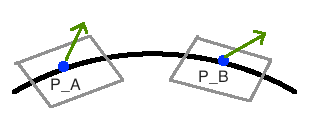
\includegraphics[width=0.5\textwidth]{images/tangent-spaces.png}
\caption{Tangent spaces}
\end{figure}

In general, we cannot compare geometric objects at $P_A$ and $P_B$ (they live in different tangent spaces) unless we have a recipe for ``moving'' geometric objects from $P_A$ to $P_B$, e.g. parallel transport (which we will consider later).

For now we just consider \underline{flat} space, where all points share a common tangent space.


Look for $\pmx{M\\N+1}$ tensor $\nabla T$ which contracts with a vector $\vec{A}$ to give infinitesimal rate of change of $T$ along $\vec{A}$. We call the rate of change $\nabla_{\vec{A}}T$ (type $\pmx{M\\N}$) the \emph{covariant derivative}
\begin{equation}
\nabla_{\vec{A}} T=\langle \nabla T,\vec{A}\rangle
\end{equation}

e.g. if $T$ is a scalar $\underbrace{\phi}_{\pmx{0\\0}\text{ type}}$, then $\nabla T=\underbrace{\tilde{d\phi}}_{\text{gradient }\pmx{0\\1}}$

e.g. if T is a vector, say $\vec{V}$: in general consider two points $P_A$, $P_B$ joined by a world line $\vec{x}(t)$

\begin{figure}[h]
\centering
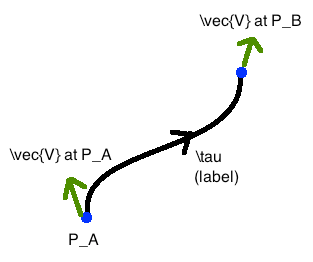
\includegraphics[width=0.5\textwidth]{images/world-line.png}
\caption{World line connecting points $P_A$ and $P_B$}
\end{figure}

\begin{align*}
\frac{d\vec{V}}{d\tau}(\vec{x}(\tau))&=\frac{d}{d\tau}\left[V^{\alpha}(\vec{x}(\tau))\vec{e}_{\alpha}
(\vec{x}(\tau))\right]\\
&=\frac{\partial V^{\alpha}}{\partial x^{\beta}}\frac{dx^{\beta}}{d\tau}\vec{e}_{\alpha}(\vec{x}(\tau))
+V^{\alpha}\frac{\partial \vec{e}_{\alpha}}{\partial x^{\beta}}\frac{dx^{\beta}}{d\tau}\qquad\text{product rule}\\
&=\left(\frac{\partial V^{\alpha}}{dx^{\beta}}\vec{e}_{\alpha}+V^{\alpha}\frac{\partial \vec{e}_{\alpha}}{\partial x^{\beta}}\right)u^{\beta}\qquad\text{4-velocity}\label{diff eqn1}
\end{align*}

The parts inside the brackets of (\ref{diff eqn1}), denoted as $(\ldots)$, are contracted with $\vec{u}$ to give the LHS, which is a vector. So $(\ldots)$ is type $\pmx{1\\1}$.

$\frac{\partial \vec{e}_{\alpha}}{\partial x^{\beta}}$ are vectors, so can be written as a linear combination of basis vectors. 

\begin{equation}
\text{Define: } \frac{\partial \vec{e}_{\alpha}}{\partial x^{\beta}}=\Gamma^{\mu}_{\alpha\beta} \vec{e}_{\mu}\label{de dx with chris}
\end{equation}

Then,

\begin{align*}
(\ldots)&=\frac{\partial V^{\alpha}}{\partial x^{\beta}}\vec{e}_{\alpha} + V^{\alpha}\Gamma^{\mu}_{\alpha\beta}\vec{e}_{\mu}\\
&=\left(\frac{\partial V^{\alpha}}{\partial x^{\beta}}+\Gamma^{\alpha}_{\mu\beta}V^{\mu}\right)
\vec{e}_{\alpha}
\end{align*}

The bracketed part above is, in index notation, $V^{\alpha}_{; \beta}$; the components of covariant derivation $\nabla \vec{V}$ of type $\pmx{1\\1}$.

Notation: switch $\mu \leftrightarrow \alpha$ in \underline{dummy} index (repeated).

Christoffel symbols $\Gamma$:
\begin{itemize}
\item $4\times 4\times 4=64$ numbers
\item solve 64 equations given by (\ref{de dx with chris}) - linear equations (easy to solve!)
\begin{itemize}
\item an alternative trick is to use the metric, which we will see later
\end{itemize}
\item are Christoffel symbols components of a $\pmx{1\\2}$ tensor?
\begin{itemize}
\item No!
\item $\{\Gamma^{\mu}_{\alpha\beta}\vec{e}_{\mu}\}$ are components of a tensor, but the $\Gamma$'s themselves are not
\item e.g. is $\Gamma$'s are tensor, then
\begin{equation}
\Gamma^{\mu'}_{\alpha' \beta'}=\frac{\partial x^{\mu'}}{\partial x^{\mu}}\frac{\partial x^{\alpha}}{\partial x^{\alpha'}}\frac{\partial x^{\beta}}{\partial x^{\beta'}}\Gamma^{\mu}_{\alpha\beta}\label{tensor Chris}
\end{equation}
\item but from the definition of $\Gamma$'s we have $\Gamma^{\mu}_{\alpha\beta}=0$ for (say) Cartesian coordinates, which would then wrongly imply $\Gamma^{\mu'}_{\alpha'\beta'}$ from (\ref{tensor Chris}) too!
\end{itemize}
\end{itemize}

Physically: suppose you have a vector $\vec{V}$ which does \underline{not} change from point to point. We want $\nabla \vec{V}=0$.

\begin{figure}[h]
\centering
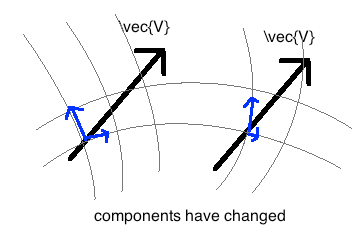
\includegraphics[width=0.5\textwidth]{images/vectors-v.png}
\caption{Vectors V}
\label{Christoffel image}
\end{figure}

If the coordinates are curvilinear, then components ``artificially'' change. The $\Gamma$'s ``undo'' the artificial change!


\review{
\begin{align*}
T&=\pmx{M\\N}\text{ tensor}\\
\nabla T&=\pmx{M\\N+1}\text{ tensor}\\
\nabla_{\vec{A}}T&=\text{covariant derivative of T along }\vec{A}=\langle\nabla T,\vec{A}\rangle=\text{type }\pmx{M\\N}
\end{align*}

e.g. if $T$ of a scalar $\phi$ then $\nabla T=\tilde{d\phi}$

e.g. if $T$ is a vector $\vec{V}$ then $\nabla \vec{V}$ is a $\pmx{1\\1}$ object
\begin{equation}
\underbrace{(\nabla \vec{V})^{\alpha}_{\beta}}_{\text{notation: }V^{\alpha}_{;\beta}}=
\underbrace{\frac{\partial V^{\alpha}}{\partial x^{\beta}}}_{\text{notation: }V^{\alpha}_{,\beta}}
+\underbrace{\Gamma^{\alpha}_{\lambda\beta}}_{\text{Christoffel}}V^{\lambda}
\end{equation}

Christoffel symbol corrects for artificial change in components of $\vec{V}$ due to curvilinear coordinates (see Figure \ref{Christoffel image}). Derived for curvilinear coordinates in flat space but remains true for curved spaces also!

\underline{Note:} neither $V^{\alpha}_{,\beta}$ nor $\Gamma^{\mu}_{\alpha\beta}$ are tensors ($\Gamma$'s are components of set of tensors $\{\nabla \vec{e}_{\alpha}\}$). But $V^{\alpha}_{;\beta}$
}

\subsection{Covariant derivative of 1-form}
What about 1-forms? Can we just say

\begin{equation*}
p_{\alpha;\beta}=\frac{\partial p_{\alpha}}{\partial x^{\beta}}
+\Gamma^{\alpha}_{\lambda\beta}p_{\lambda}\quad \text{??}
\end{equation*}

No, we cannot - note the double lowered $\lambda$ in the RHS.

$\nabla\tilde{p}$ is $\pmx{0\\2}$ type/

We redo rate-of-change calculation along world line $\vec{x}$
\begin{align}
\frac{d\tilde{p}}{d\tau}&=\frac{d}{d\tau}\left[p_{\alpha}(\vec{x}(\tau))\tilde{\omega}^{\alpha}(\vec{x}(\tau))\right]\\
&=\frac{\partial p_{\alpha}}{dx^{\beta}}\frac{dx^{\beta}}{d\tau}\tilde{\omega}^{\alpha}+p_{\alpha}\underbrace{\frac{\partial \tilde{\omega}^{\alpha}}{\partial x^{\beta}}}_{\text{1-form}}
\frac{dx^{\beta}}{d\tau}
\end{align}

We can write the 1-form as linear combination $x_{\mu\beta}^{\alpha}\tilde{\omega}^{\mu}$

Are $x$'s related to $\Gamma$;s? Yes - duality.
\begin{equation}
\delta ^{\alpha}_{\beta}=\langle \tilde{\omega}^{\alpha},\vec{e}_{\beta}\rangle\qquad \text{from previous lectures}
\end{equation}

Differentiate by $x^{\gamma}$
\begin{align}
0&=\langle\frac{\partial\tilde{\omega}^{\alpha}}{\partial x^{\gamma}},\vec{e}_{\beta}\rangle 
\langle \tilde{\omega}^{\alpha},\frac{\partial \vec{e}_{\beta}}{\partial x^{\gamma}}\\
&=\langle x_{\mu\gamma}^{\alpha}\tilde{\omega}^{\mu},\vec{e}_{\beta}\rangle +\langle\tilde{\omega}^{\alpha},\Gamma^{\lambda}_{\beta\gamma}\vec{e}_{\lambda}\rangle\\
&=x^{\alpha}_{\mu\gamma}\delta^{\mu}_{\beta}
+\Gamma^{\lambda}_{\beta\gamma}\delta^{\alpha}_{\lambda}\\
&=x^{\alpha}_{\beta\gamma}+\Gamma^{\alpha}_{\beta\gamma}
\end{align}
i.e. opposites!

Components of $\nabla\tilde{p}$, i.e. $(\nabla\tilde{p})_{\alpha\beta}$ is notationally $p_{\alpha;\beta}$

\begin{equation}
p_{\alpha;\beta}=\frac{\partial p_{\alpha}}{\partial x^{\beta}}-\Gamma^{\lambda}_{\alpha\beta} p_{\lambda}
\end{equation}

For general tensor: add correction term $\pm \Gamma$ tensor for each tensor index; $+$ is index is up; $-$ if index is down.

\begin{equation}
\text{e.g. } T^{\alpha}_{\beta;\gamma}=\frac{\partial T^{\alpha}_{\beta}}{\partial^{\gamma}}
+\underbrace{\Gamma^{\alpha}_{\lambda\gamma} T^{\lambda}_{\beta}}_{\text{by analogy with vector}}
-\underbrace{\Gamma^{\lambda}_{\beta \gamma}T^{\alpha}_{\lambda}}_{\text{by analogy with 1-form}}
\end{equation}

\subsection{Covariant derivative of metric}

Recall
\begin{align}
\nabla \vec{V}&=\pmx{1\\1}\text{ type}\\
\nabla \tilde{V}&=\pmx{0\\2}\text{ type}
\end{align}
where $\tilde{V}$ is the specific 1-form induced by the metric with $\vec{V}$ in the one slot ($\tilde{V}=g(\vec{V},\ldots)$).

We can go from $\pmx{0\\2}$ to $\pmx{1\\1}$ by contraction! 

Consider $\nabla_{\vec{a}}\vec{V}=\pmx{1\\0}$ object. 

Then $g(\nabla_{\vec{A}}\vec{V},\ldots)$ is a 1-form induced by $g$. 

By definition this is $\nabla_{\vec{A}}\tilde{V}$ which is a 1-form, i.e. $\nabla\tilde{V}\pmx{0\\2}$ contracted with $\vec{A}$. 

In index notation:
\begin{equation}
V_{\alpha;\beta}=g_{\alpha\gamma}V^{\gamma}_{;\beta}\qquad\text{as in previous lectures}
\end{equation}


\subsection{Christoffel Symbols and Metric and Acceleration}
\subsubsection{Covariant derivative}
$\nabla g$ is a $\pmx{0\\3}$ tensor (with components $g_{\alpha\beta ; \gamma}$).

From last time, given $\vec{V}$ there is a $\tilde{V}$.

By definition,
\begin{equation}
V_{\alpha;\beta}=g_{\alpha\gamma} V^{\gamma}_{;\beta}\quad\text{(or $\nabla_{\vec{A}}\vec{V}$)}\label{product rule}
\end{equation}

Separately,
\begin{equation}
V_{\alpha}=g_{\alpha\beta}V^{\gamma}\label{Valph}
\end{equation}

Taking the covariant derivative of both sides of (\ref{Valph}) with respect to $x^{\beta}$
\begin{align}
\Rightarrow V_{\alpha;\beta}&=g_{\alpha\gamma;\beta}V^{\gamma}+g_{\alpha\gamma}V^{\gamma}_{;\beta}\\
&\Rightarrow g_{\alpha\gamma;\beta=0}\\
&\Rightarrow \nabla g=0
\end{align}

We can use this to get a formula for $\Gamma$'s ($\Gamma$'s are coefficients in linear combination of basis vectors which give $\frac{\partial \vec{e}_{\alpha}}{\partial x_{\beta}}$)

An alternative derivation of $\nabla g=0$:

In flat space, $g_{\alpha\beta , \gamma}=0$ \underline{and} $\Gamma$'s are zero because $\frac{\partial\vec{e}_{\alpha}}{\partial x^{\beta}}=0$
\begin{align}
\Rightarrow g_{\alpha\beta;\gamma}&=g_{\alpha\beta,\gamma}-(\text{two terms involving Christoffel symbols})\\
&=0 \quad\text{in flat space}
\end{align}

But $g_{\alpha\beta;\gamma}=0$ involves only decent tensors, so it's free in ????

\begin{equation}
-=g_{\alpha\beta;\gamma}=g_{\alpha\beta,\gamma}-\Gamma^{\lambda}_{\alpha\gamma}g_{\lambda\beta}
\end{equation}

??? gives us 64 equations for 64 unknowns ($\Gamma$ components) provided $g_{\alpha\beta}$ and $g_{\alpha\beta,\gamma}$ are given.

Simplification: symmetric in $\alpha,\beta$; symmetric in lower indices of the $\Gamma$'s

Using this and write three cyclic permutations of (*) and sum them (see Schutz p. 142):

\begin{equation}
\Gamma^{\lambda}_{\alpha\beta}=\frac{1}{2}g^{\lambda\mu}(g_{\mu\alpha,\beta}+g_{\mu\beta,\alpha}-g_{\alpha\beta,\mu})\label{chris to mem}
\end{equation}
You should memorise equation (\ref{chris to mem})!

\begin{itemize}
\item If Minkowski:
\begin{itemize}
\item $\Gamma$'s are 0
\end{itemize}
\item If not:
\begin{itemize}
\item $\Gamma\text{'s}\neq 0$, coordinates are curved, but space may not be curved
\end{itemize}
\end{itemize}

Curvatures of manifold depend on 2nd derivatives of g.

\subsection{The 4-acceleration}
$\vec{u}=\frac{d\vec{x}}{d\tau}$ is a first derivative (i.e. this is calculated without reference to curvature of coordinates and/or manifold).

$\vec{a}$ is a second derivative. We need to refer to curvature of coordinates/manifold.

In general, $\vec{a}=\nabla_{\vec{u}}\vec{u}$, i.e. rate of change of $\vec{i}$ along itself.

In free fall: $\nabla_{\vec{u}}\vec{u}=0$ (but with rocket engines $\nabla_{\vec{u}}\vec{u}\neq 0$)

Christoffel symbols contain curvature!

\review{Last lecture: \begin{itemize}
\item $\Gamma^{\lambda}_{\alpha\beta}=\frac{1}{2}g^{\lambda\mu}(g_{\mu\alpha,\beta}+g_{\mu\beta,\alpha}-g_{\alpha\beta,\mu})$
\item $g_{\alpha\beta;\gamma}=0$
\end{itemize}
}

Remember, for curved space, 4-acceleration $\vec{a}\neq\frac{d^2\vec{x}}{d\tau^2}$. This is the derivative of $x^{\alpha}(\vec{e}_{\alpha})$ not just coordinates. $\tau$ involves curvature.

For free fall, $\vec{a}=0$ (compare with Newtonian $\SI{9.8}{ms^{-2}}$

\example{?}{Astronaut above Schwarz. black hole, at distance $r$ (radial coordinate appearing in metric), with $\theta$ and $\phi$ also fixed. The Schwarzchild metric is:
\begin{align}
g_{tt}&=-\left(1-\frac{2M}{r}\right)\\
g_{rr}&=\left(1-\frac{2M}{r}\right)^{-1}\\
g_{\theta\theta}&=...\\
g_{\phi\phi}&=...
\end{align}

Note: rotating black hole is not diagonal! (but it will be symmetric because $A^{\alpha}\vec{e}_{\alpha}=A^{\beta}\vec{e}_{\beta}$; non-diagonal $\Leftarrow$ diagonal (one way!))

Question: what is the acceleration of this astronaut (globally not flat) at a fixed radius?

We need $\vec{u}=\left(\frac{dt}{d\tau},0,0,0\right)$

\begin{align}
\vec{x}&=(t,r,\theta,\phi)\\
\vec{u}&=\frac{d\vec{x}}{d\tau}
\end{align}

What is $u_t$? We need to normalise.

\begin{align}
\vec{u}\cdot\vec{u}&=-1\\
u^\beta g^{\alpha\beta}u_{\alpha}&=-\left(1-\frac{2M}{r}\right)=u_t^2=-1\\
&\Rightarrow u_t=\left(1-\frac{2M}{r}\right)^{-1/2}
\end{align}

\begin{align}
a^{\alpha}&=u^{\beta}u^{\alpha}_{;\beta}\quad\text{covariant derivative}\\
&=u^{\beta}\left(\frac{\partial u^{\alpha}}{\partial x^{\beta}}+\Gamma^{\alpha}_{\lambda\beta}u^{\lambda}\right)\\
&=\underbrace{\frac{\partial u^{\alpha}}{\partial\tau}}_{\text{zero}}+\Gamma^{\alpha}_{\lambda\beta}u^{\lambda}u^{\beta}
\end{align}

Now,
\begin{align}
a^t=a^{\theta}=a^{\phi}&=0\\
\Rightarrow a^{r}&=\Gamma^{r}_{tt}(u^t)^2\\
&=\frac{M}{r^2}\left(1-\frac{2M}{r}\right)\cdot\left[\left(1-\frac{2M}{r}\right)^{-1/2}\right]^2=\frac{M}{r^2}
\end{align}

\begin{equation}
\vec{a}=\nabla_{\vec{u}}\vec{u}=(0,\frac{M}{r^2},0,0)=\frac{M}{r^2}\hat{r}\quad\text{(accelerating outwards!)}
\end{equation}

We will prove that acceleration is always orthogonal to the 4-velocity.

\begin{align}
\vec{u}\cdot\vec{u}&=-1=u^{\alpha}u_{\alpha}
\intertext{Take the covariant derivative}
\Rightarrow 0&=(u^{\alpha}_{;\beta}u_{\alpha}+u^{\alpha}u_{\alpha;\beta})u^{\beta}\\
&=(u^{\alpha}_{;\beta}u_{\alpha}+u_{\gamma}g^{\gamma\alpha}u_{\alpha;\beta})u^{\beta}\quad\text{(note $g^{\gamma\alpha}_{;\beta}=0$)}\\
0&=(u^{\alpha}_{;\beta}u_{\alpha}+u_{\gamma}u^{\gamma}_{;\beta})u^{\beta}
\end{align}
where we have switched co- and contra-variant indices using the metric!

So $(u_\alpha u^{\alpha}_{;\beta})u^{\beta}=0$ (both terms are equal).
\begin{equation}
\Rightarrow \vec{u}\cdot\vec{a}=0
\end{equation}
}


\subsection{Fermi-Walker Transport}

What does the ``natural basis'' of an observer in a rocket ship $(\vec{a},\vec{v})$ in curved space look like, compared to some external basis? (global coordinate system)

We let $\vec{v}$ be an arbitrary vector. We then solve
\begin{equation}
\nabla_{\vec{u}}\vec{v}=(\vec{a}\cdot\vec{v})\vec{u}-\vec{a}(\vec{u}\cdot\vec{v})
\end{equation}
to see what $\vec{v}$ and $\vec{u}$ look like in a global coordinate system.

Not unique apparently. However,
\begin{enumerate}
\item 
\begin{equation}
\nabla_{\vec{u}}(\vec{v}\cdot\vec{v})=2\vec{v}\cdot\nabla_{\vec{u}}\vec{v}=0\quad\text{lengths preserved}
\end{equation}
\item 
\begin{equation}
\nabla_{\vec{u}}(\vec{v}\cdot\vec{w})=\vec{v}\cdot\nabla_{\vec{u}}\vec{w}+\vec{w}\cdot\nabla_{\vec{u}}\vec{v}=0
\quad\text{angles preserved (orthogonality)}
\end{equation}
\item
4-velocity is Fermi-Walker transported automatically. (if $\vec{v}=\vec{u}$ then
\begin{align}
\nabla_{\vec{u}}\vec{v}&=(\vec{a}\cdot\vec{u})\vec{u}-\vec{a}(\vec{u}\cdot\vec{u})\\
&=\vec{a}\quad\text{identically satisfied}
\end{align}
You can treat your time axis to be $\vec{u}$ (along the path).
\item
If $\vec{w}$ is spacelike (orthogonal to $\vec{a}$ and $\vec{u}$), then $\nabla_{\vec{u}}\vec{w}=0$ ($\vec{w}$ does not rotate spatially relative to $\vec{u}$) (it's temporal (?))
\end{enumerate}

\subsection{Constants of motion}

Approach \#1: use Lagrangian methods

Approach \#2: for free fall
\begin{equation}
\nabla_{\vec{u}}\vec{u}=0 \label{freefall crit}
\end{equation}
(for a photon $\nabla_{\vec{p}}\vec{p}=0$)
We can also look at the 1-form version of equation (\ref{freefall crit})
\begin{equation}
\nabla_{\vec{u}}\tilde{u}=0
\end{equation}
\begin{align}
\text{Components: }\quad&u^{\beta}_{\alpha;\beta}=0\\
&\underbrace{u^{\beta}}_{=\frac{\partial x^{\beta}}{d\tau}}
\left(\frac{\partial u_{\alpha}}{\partial x^{\beta}}-\Gamma^{\lambda}_{\alpha\beta}u^{\lambda}\right)=0
\end{align}

\begin{equation}
\text{i.e., } \underbrace{\frac{\partial u_{\alpha}}{d\tau}}_{\text{chain rule}}
=\Gamma^{\lambda}_{\alpha\beta}u_{\lambda}u^{\beta}
\end{equation}

\begin{align}
\text{Recall: }\quad&&\Gamma^{\lambda}_{\alpha\beta}&=\frac{1}{2}g^{\lambda\mu}
(g_{\mu\alpha,\beta}+g_{\mu\beta,\alpha}-g_{\alpha\beta,\mu})\\
&&\Gamma^{\lambda}_{\alpha\beta}u_{\lambda}u^{\beta}
&=\frac{1}{2}\underbrace{u^{\mu}u^{\beta}}_{\text{symm. }\mu\leftrightarrow \beta}
(g_{\mu\alpha,\beta}+g_{\mu\beta,\alpha}-g_{\alpha\beta,\mu})
\intertext{Now, $g_{\mu\alpha,\beta}$ and $g_{\alpha\beta,\mu}$ are antisymmetric under exchange of $\mu\leftrightarrow\beta$}
&&&=\frac{1}{2}u^{\mu}u^{\beta}g_{\mu\beta,\alpha}
\end{align}
since contraction of symmetric and antisymmetric components vanishes.

i.e., if the metric is independent of coordinate $x^{\alpha}$ then $u_{\alpha}$ is constant along world line.

e.g., in Schwarz spacetime, a freely falling body has $u_{\phi}=\text{constant}$ and $u_t=\text{constant}$.


\subsection{Polar coordinates}

We shall explore polar coordinates through use of an example.

Polar coordinates (primed): $(r,\theta)$

Cartesian (unprimed): $(x,y)$
\begin{align}
x&=r\cos\theta\\
y&=r\sin\theta
\end{align}

Our plan is:
\begin{itemize}
\item get polar basis
\item get polar metric
\item get polar Christoffel symbol
\end{itemize}

To get \textbf{polar basis}:

Transformation matrix:
\begin{align}
\frac{\partial x^{\alpha}}{\partial x^{\alpha'}}&=\pmx{\frac{\partial x}{\partial r}&\frac{\partial x}{\partial \theta}\\
\frac{\partial y}{\partial r}&\frac{\partial y}{\partial \theta}}=\pmx{\cos\theta&-r\sin\theta\\\sin\theta&r\cos\theta}\\
\frac{\partial x^{\alpha'}}{\partial x^{\alpha}}&=\pmx{\frac{\partial r}{\partial x}&\frac{\partial r}{\partial y}\\
\frac{\partial \theta}{\partial x}&\frac{\partial \theta}{\partial y}}=\ldots \quad\text{exercise}
\end{align}


Basis vectors:
\begin{align}
\vec{e}_{\alpha}&=\frac{\partial x^{\alpha'}}{\partial x^{\alpha}}\vec{e}_{\alpha'}\\
\vec{e}_r&=\frac{\partial x}{\partial r}\vec{e}_x+\frac{\partial y}{\partial r}\vec{e}_y\\
&=\cos\theta\vec{e}_x+\sin\theta\vec{e}_y\\
\vec{e}_{\theta}&=\frac{\partial x}{\partial \theta}\vec{e}_x+\frac{\partial y}{\partial \theta}\vec{e}_y\\
&=-r\sin\theta\vec{e}_x+r\cos\theta \vec{e}_y
\end{align}

\begin{center}[h]

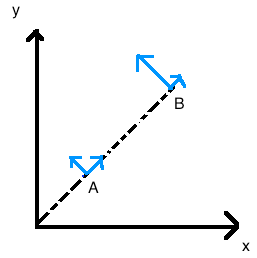
\includegraphics[width=0.5\textwidth]{images/polar.png}
\captionof{figure}{Polar coordinates?}
\label{polar coords fig}
\end{center}
 
In Figure \ref{polar coords fig} above we see the vector length at $B$ is greater than at $A$; the length of $\vec{e}_\theta$ is proportional to $r$ because we need to subtend a greater arc further out so as to produce unit change in $\theta$.


\textbf{Polar metric}:
\begin{align}
g_{\alpha'\beta'}&=\vec{e}_{\alpha'}\vec{\beta'}\\
g_{rr}&=\vec{e}_r\cdot\vec{e}_r=1\\
g_{r\theta}&=\vec{e}_r\cdot \vec{e}_{\theta}=0\\
g_{\theta\theta}&=\vec{e}_{\theta}\cdot\vec{e}_{\theta}=r^2
\end{align}

\exercise{
Check this this also follows from the transformation law
\begin{equation}
g_{\alpha'\beta'}=\frac{\partial x^{\alpha}}{\partial x^{\alpha'}}\frac{\partial x^{\beta}}{\partial x^{\beta'}}
\underbrace{g_{\alpha\beta}}_{\pmx{1&0\\0&1}\text{ Cartesian}}
\end{equation}
}
{}

Christoffel symbols describe derivatives of basis vectors in that basis itself

\begin{align}
\frac{\partial \vec{e}_r}{\partial r}&=0\\
\frac{\partial \vec{e}_r}{\partial \theta}&=-\sin\theta\vec{e}_x+\cos\theta \vec{e}_y\\
\frac{\partial \vec{e}_{\theta}}{\partial r}&=-\sin\theta\vec{e}_x+\cos\theta\vec{e}_y\\
\frac{\partial \vec{e}_{\theta}}{\partial \theta}&=-r\cos\theta \vec{e}_x-r\sin\theta\vec{e}_y
\end{align}

Expressing these in the basis we get
\begin{center}
\begin{tabular}{l|l|l}
$\frac{\partial \vec{e}_r}{\partial r}=0$ & $\Gamma^{r}_{rr}=0$&$\Gamma^{\theta}_{rr}=0$\\
$\frac{\partial \vec{e}_r}{\partial \theta}=\frac{1}{r}\vec{e}_\theta$ & $\Gamma^{r}_{r\theta}=0$&$\Gamma^{\theta}_{r\theta}=\frac{1}{r}$\\
$\frac{\partial \vec{e}_{\theta}}{\partial r}=\frac{1}{r}\vec{e}_{\theta}$ & $\Gamma^{r}_{\theta r}=0$&$\Gamma^{\theta}_{\theta r}=\frac{1}{r}$\\
$\frac{\partial \vec{e}_{\theta}}{\partial \theta}=-r\vec{e}_r$ & $\Gamma^{r}_{\theta\theta}=-r$&$\Gamma^{\theta}_{\theta \theta}=0$\\
\end{tabular}
\end{center}

Important to recall:
\begin{equation}
\frac{\partial \vec{e}_{\alpha}}{\partial x^{\beta}}=\vec{e}_{\mu}\Gamma^{\mu}_{\alpha\beta}
\end{equation}

We should check this works when taking covariant derivative of $\vec{V}$.

Special case: $\vec{V}=\vec{e}_{x}=\text{constant}$. We should find $\nabla_{\vec{A}}\vec{V}=0$ for all $\vec{A}$.

To check: we write $\vec{V}$ in polar coordinates:
\begin{equation}
\vec{V}=\cos\theta\vec{e}_{r}-\frac{1}{r}\sin\theta\vec{e}_{\theta}
\end{equation}
from transformation laws for basis vectors.

\begin{align*}
\left(\nabla_{\vec{A}}\vec{V}\right)^{\alpha}&=A^{\beta}\left(\frac{\partial V^{\alpha}}{\partial x^{\beta}}+\Gamma^{\alpha}_{\lambda\beta}V^{\lambda}\right)\\
\therefore \left(\nabla_{\vec{A}}\vec{V}\right)^{r}&=A^{\beta}\frac{\partial V^{r}}{\partial x^{\beta}}+\Gamma^r_{\lambda\beta}V^{\lambda}A^{\beta}\\
&=A^{\theta}\frac{\partial V^r}{\partial \theta}+\Gamma^{r}_{\theta\theta}V^{\theta}A^{\theta}\quad\text{other terms zero}\\
&=A^{\theta}(-\sin\theta)-r\cdot\left(-\frac{1}{r}\sin\theta\right)A^{\theta}\\
&=0\\
\left(\nabla_{\vec{A}}\vec{V}\right)^{\theta}&=A^{\beta}\frac{\partial V^{\theta}}{\partial x^{\beta}}+\Gamma^{\theta}_{\lambda\beta}V^{\lambda}A^{\beta}\\
&=A^r\frac{\partial V^{\theta}}{\partial r}+A^{\theta}\frac{\partial V^{\theta}}{\partial \theta}+\Gamma^{\theta}_{r\theta}V^{r}A^{\theta}+\Gamma^{\theta}_{\theta r}V^{\theta}A^{r}\\
&=A^{r}\cdot\frac{1}{r^2}\sin\theta+A{\theta}\cdot\left(-\frac{\cos\theta}{r}\right)+\frac{1}{r}\cdot\cos\theta\cdot A^{\theta}+\frac{1}{r}\left(-\frac{1}{r}\sin\theta\right)A^r\\
&=0
\end{align*}

\exercise{Metric $g=\text{diag}(1,r^2)$ from previous lecture; check that $\nabla g=0$ explicitly.}{}

\exercise{Confirm that $\Gamma$'s can also be derived from
\begin{equation}
\Gamma^{\mu}_{\alpha\beta}=\frac{1}{2}g^{\mu\lambda}(g_{\lambda\alpha,\beta}+g_{\lambda\beta,\alpha}
-g_{\alpha\beta,\lambda})
\end{equation}}{}

\exercise{Prove divergence
\begin{equation}
V^{\alpha}_{;\alpha}=\frac{1}{r}\frac{\partial}{\partial r}(rV_r)+\frac{\partial V_{\theta}}{\partial \theta}
\end{equation}
as you would expect from undergrad.}{}

\exercise{Derive $\chi^{\mu}_{\alpha\beta}$'s for basis one-forms
\begin{align}
\tilde{\omega}^r&=\cos\theta\cdot\tilde{\omega}^x+\sin\theta\cdot\tilde{\omega}^y\\
\tilde{\omega}^{\theta}&=-\frac{\sin\theta}{r}\cdot\tilde{\omega}^x+\frac{\cos\theta}{r}\cdot\tilde{\omega}^y
\end{align}}{}


\section{Curved space}

In the presence of gravity, we cannot have a global inertial (Minkowski) frame.

\begin{figure}[h]
\centering
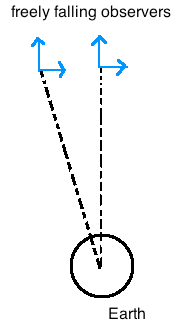
\includegraphics[height=0.2\textheight]{images/freely-falling-observers.png}
\caption{Freely falling observers}
\end{figure}
We see that the distance between the observers decreases! i.e. curved geodesics $\Rightarrow$ curved space!

\subsection{Curved manifold}
\begin{itemize}
\item Extrinsic curvature: is space curved with respect to the space in which it's embedded?
\begin{figure}[h]
\centering
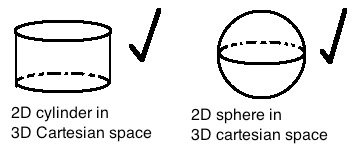
\includegraphics[width=0.5\textwidth]{images/extrinsic-curvature.png}
\caption{Extrinsic curvature}
\end{figure}\\
Yes!
\item Intrinsic curvature: without refernce to an emedding. Do neighbouring geodesics (``free fall'') diverge/converge? Note we need the idea of parallel transport to discuss geodesics.
\begin{figure}[h]
\centering
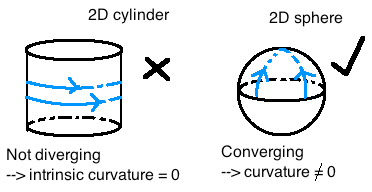
\includegraphics[width=0.5\textwidth]{images/intrinsic-curvature.png}
\caption{Intrinsic curvature}
\end{figure}\\
We see that a 2D cylinder does \underline{not} have intrinsic curvature!
\end{itemize}

\subsection{Local flatness}
\begin{itemize}
\item Let $\{x^{\alpha}\}$ be some generic coordinates
\item Make a transformation to $\{x^{\alpha'}\}$ coordinates
\item See how for we can get in flattening the space near a point $\hat{x}_0$
\item Can we choose $x^{\alpha'}(\vec{x})$ in such a way that the primed metric is Minkowski near $\vec{x}_0$?
\begin{itemize}
\item exactly no, but approximately yes
\end{itemize}
\end{itemize}

\underline{At $\vec{x}_0$}:

We are in a tangent space; first derivatives of the metric at the second derivatives disappear.

\underline{Away from $\vec{x}_0$}:

Curvature contributes to $\vec{a}$ (we can set first derivatives to metric to zero)

To transform from primed to unprimed:
\begin{equation}
\Lambda^{\alpha}_{\mu'}=\frac{\partial x^{\alpha}}{\partial \mu'}
\end{equation}

Aim: to compute transformed metric
\begin{equation}
g_{\mu'\nu'}=\Lambda^{\alpha}_{\mu'}\Lambda^{\beta}_{\nu'}g_{\alpha\beta}
\end{equation}
We seek to cheek $x^{\alpha'}$ (and hence $\Lambda^{\alpha}_{\mu'}$) in order to make $g_{\mu'\nu'}$ as flat as possible.

Taylor expansion: small departures around $\vec{x}_0$; no cusps, space is differentiable, order of differentiation is unimportant.
\begin{align}
\Lambda^{\alpha}_{\mu'}&=\Lambda^{\alpha}_{\mu'}\rvert_{\vec{x}_0}
+\frac{\partial \Lambda^{\alpha}_{\mu'}}{\partial x^{\gamma'}}\left(x^{\gamma'}-x^{\gamma'}_0
+\frac{1}{2}\frac{\partial^2 \Lambda^{\alpha}}{\partial x^{\gamma'}~\partial x^{\delta'}}
\left(x^{\gamma'}-x_0^{\gamma'}\right)(x^{\delta'}-x_0^{\delta'}\right)+\ldots\\
&=\Lambda^{\alpha}_{\mu'}\rvert_{\vec{x}_0}+\frac{\partial}{\partial x^{\gamma'}}
\left(\frac{\partial x^{\alpha}}{\partial \mu'}\right)\rvert^{(x^{\gamma'}-x_0^{\gamma'}}_{\vec{x}_0}
+\frac{1}{2}\frac{\partial^3 x^{\alpha}}{\partial x^{\mu'}~\partial x^{\gamma'}~\partial x^{\delta'}}\rvert_{\vec{x}_0}
\left(x^{\gamma'}-x_0^{\gamma'}\right)\left(x^{\delta'}-x_0^{\delta'}\right)+\ldots\\
g_{\alpha\beta}&=g_{\alpha\beta}\rvert_{\vec{x}_0}+g_{\alpha\beta,\gamma'}\left(x^{\gamma'}-x_0^{\gamma'}\right)
+\frac{1}{2}g_{\alpha\beta,\gamma'\delta'}\left(x^{\gamma'}-x_0^{\gamma'}\right)
\left(x^{\delta'}-x_0^{\delta'}\right)+\ldots
\intertext{Therefore, at zeroth order}
g_{\mu'\nu'}&=\Lambda^{\alpha}_{\mu'}\rvert_{\vec{x}_0}~\Lambda^{\beta}_{\nu'}\rvert_{\vec{x}_0}~
g_{\alpha\beta}\rvert_{\vec{x}_0}
\end{align}

(Can we make this flat?)

\subsection{Miscellaneous practical results}
On curved space times.

\subsubsection{Proper length}
Also called the ``geodesic length''

\begin{equation}
ds^2=g_{\alpha\beta}\frac{dx^{\alpha}(\lambda)}{d\lambda}\cdot \frac{dx^{\beta}(\lambda)}{d\lambda}
\end{equation}
\begin{equation}
\text{proper length}=\int^{\lambda_1}_{\lambda_0}dx~\sqrt{\frac{d\vec{x}}{d\lambda}\cdot\frac{d\vec{x}}{d\lambda}}
\end{equation}
Proper length is coordinate independent.

\subsubsection{Volume}

\begin{align}
\text{Inifinitesimal volume}&=dx^{0'}~dx^{1'}~dx^{2'}~dx^{3'}\\
&=\text{Jacobian}\times dx^0~dx^1~dx^2~dx^3\\
&=\det\underbrace{\left(\frac{\partial x^{\alpha'}}{\partial x^{\alpha}}\right)}
_{\Lambda^{\alpha'}_{\alpha}} dx^0~dx^1~dx^2~dx^3
\end{align}

For an infinitesimal volume: locally the manifold is flat. So there exists a transformation that maps $g$ into Minkowski $\eta$.

In matrix notation:
\begin{equation}
g=\Lambda\eta\Lambda^{\top}
\end{equation}

In component notation:
\begin{equation}
g_{\alpha\beta}=\Lambda^{\alpha'}_{\alpha}\Lambda^{\beta'}_{\beta}\eta_{\alpha'\beta'}
\end{equation}

Determinant of both sides (in matrix notation)
\begin{align}
\det g&=\det\Lambda~\det \eta ~ \det(\Lambda^{\top})\\
&=-(\det \Lambda)^2
\end{align}

Therefore $\det\Lambda=(-\det g)^{1/2}$.

\subsubsection{Divergence of a vector}
Used in conservation laws.

\begin{align}
V^{\alpha}_{;\beta}&=\frac{\partial V^{\alpha}}{\partial x^{\beta}}=\Gamma^{\alpha}_{\lambda\beta}V^{\lambda}\\
\div \vec{V}&=V^{\alpha}_{;\alpha}\\
&=\frac{\partial V^{\alpha}}{\partial x^{\alpha}}+\Gamma^{\alpha}_{\lambda\alpha}V^{\lambda}
\intertext{}
\Gamma^{\alpha}_{\lambda\beta}&=\frac{1}{2}g^{\alpha\mu}
\left(g_{\mu\lambda,\beta}+g_{\mu\beta,\lambda}-g_{\lambda\beta,mu}\right)\\
\Rightarrow \Gamma^{\alpha}_{\lambda\alpha}&+\frac{1}{2}g^{\alpha\mu}
\left(g_{\mu\lambda,\alpha}+g_{\mu\alpha,\lambda}-g_{\lambda\alpha,\mu}\right)\\
&=\frac{1}{2}g^{\alpha\mu}g_{\mu\alpha,\lambda}
\end{align}

An example: $g^{-1}g=1$ and matrix algebra.

\begin{align}
\to (\det g)_{,\mu}&=\det g-g^{\alpha\beta} g_{\alpha\beta,\mu}
\intertext{Hence}
\Gamma^{\alpha}_{\lambda\alpha}&=\frac{(\sqrt{-g})_{,\lambda}}{\sqrt{-g}}
\end{align} 
where $g\equiv \det(g_{\alpha\beta})$.

So,
\begin{equation}
\div \vec{V}=\frac{1}{\sqrt{-g}}\left(\sqrt{-g}V^{\alpha}\right)
\end{equation}

Exercise: 3D spherical polar, $g=\det(g_{\alpha\beta})=r^2\sin\theta$.

\subsubsection{Gauss Law in integral form}

\begin{equation}
\int d^3\mathbf{x'}~\div'(\mathbf{V})=\int \underbrace{d^2 \mathbf{x'}}_{dA~\mathbf{\hat{n}}}\cdot \mathbf{V}
\end{equation}

This is 4D! let's measure conservation of the quantity $\vec{V}$ locally in flat space.
\begin{equation}
0=V^{\alpha}_{,\alpha}
\end{equation}

Locally flat $\Rightarrow$ Christoffel symbols for the unprimed flat coordinates are zero
\begin{equation}
V^{\alpha}_{,\alpha}=V^{\alpha}_{,\alpha}+\underbrace{\Gamma^{\alpha}_{\lambda\alpha}
V^{\lambda}}_{\text{zero}}=V^{\alpha}_{;\alpha}
\end{equation}

Integrate over small volume in flat space
\begin{align}
\int d^4 x~ V^{\alpha}_{,\alpha}&=\int d^4 x~V^{\alpha}_{;\alpha},\quad\text{as above}
\intertext{transform into primed (non-flat) coordinates)}
&=\int d^4 x' \underbrace{\sqrt{-g}}_{\mathclap{\text{Jacobian of transform}}} \overbrace{V^{\alpha'}_{;\alpha'}}^
{\mathclap{\text{unchanged; frame invariant}}}\\
&-\int d^4 x'~\sqrt{-g}\cdot\frac{1}{\sqrt{-g}}\cdot\left(\sqrt{-g}V^{\alpha'}\right)_{,\alpha'}\\
&=\int d^4 x'~\left(\sqrt{-g} V^{\alpha'}\right)_{,\alpha'}\\
&=\int d^3 \mathbf{x'}~n_{\alpha'} V^{\alpha'}\sqrt{-g}
\end{align}
where $n_{\alpha'}$ is normal to the 3-surface enclosing the 4-volume.

This is Gauss' law (also applies to the covariant derivative).

\subsubsection{Angles}

\begin{align}
\frac{\vec{A}\cdot\vec{B}}{\lvert \vec{A}\rvert \lvert\vec{B}\rvert}&=\cos\theta
\intertext{where $\vec{A}\cdot\vec{B}=g(\vec{A},\vec{B})$}
\lvert\vec{A}\rvert&=\sqrt{g(\vec{A},\vec{A})}\\
\lvert\vec{B}\rvert&=\sqrt{g(\vec{B},\vec{B})}
\end{align}

\subsubsection{Geodesics}
Curves that continue to progress in the same direction they were progressing in; i.e. the tangent is parallel to the tangent at the previous point.
\begin{equation}
\nabla_{\frac{d\vec{x}}{d\lambda}}{d\vec{x}}{d\lambda}=0
\end{equation}
Covariant derivative of tangent along its own direction is zero.

In component notation: $\pmx{1\\0}$
\begin{align}
\frac{dx^{\beta}}{d\lambda}\left(\frac{d\vec{x}}{d\lambda}\right)^{\alpha}_{;\beta}&=0\\
\Rightarrow\frac{dx^{\beta}}{d\lambda}\left(\frac{d}{dx^{\beta}}\left(\frac{dx^{\alpha}}{d\lambda}\right)
+\Gamma^{\alpha}_{\mu\beta}\frac{dx^{\mu}}{d\lambda}\right)
&=\frac{d^2 x^{\alpha}}{d\lambda^2}+\Gamma^{\alpha}_{\mu\beta}\frac{dx^{\mu}}{d\lambda}\cdot\frac{dx^{\beta}}{d\lambda}
\end{align}

Note $\vec{x}(\lambda=0)$ and $\frac{d\vec{x}}{d\lambda}(\lambda=0)$.


\subsection{Curvature and Einstein's Field Equations}
Parallel transport!

Generally, geometric objects like vectors as different points live in different tangent spaces, hence cannot be compared. We will investigate the looks for moving them.

\subsubsection{Rules}
If $T$ is a geometric object, then we can parallel transport along $\vec{x}(\lambda)$ by requiring that
\begin{equation}
\nabla\frac{d\vec{x}}{d\lambda}T=0
\end{equation}
$\Rightarrow T$ remains constant along tangent vector (is zero ???)

An example $A \to B \to C \to A$.
\begin{figure}[h]
\centering
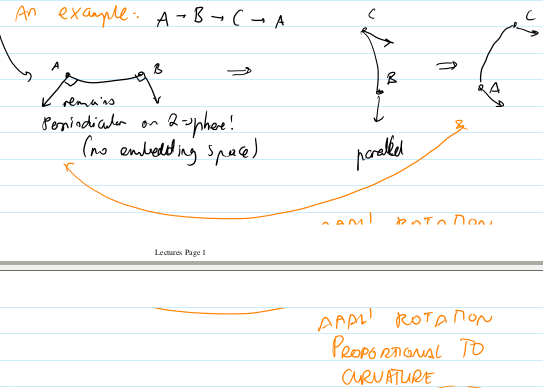
\includegraphics[width=0.5\textwidth]{images/parallel_transport_example.png}
\end{figure}

Theorem: if we parallel transport $T$ around a \underline{closed} curve, then the change in $T$ is proportional to the intrinsic curvature of the manifold (proportional to the Riemann tensor). No curvature = flat $\Rightarrow$ no change.

What is $\Delta T = T_{\text{final}} - T_{\text{initial}}$ around a closed loop? (specialise to vector $\vec{V}$)

Consider a small patch (not flat)
An example $A \to B \to C \to A$.

\begin{figure}[h]
\centering
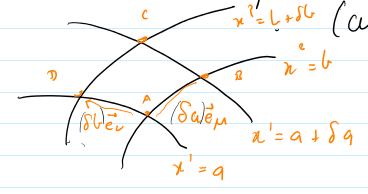
\includegraphics[width=0.5\textwidth]{images/small_patch.png}
\end{figure}

To parallel transport $\vec{V}$ around the loop $A \to B \to C \to D \to A$:

Consider AB:
\begin{align}
\nabla_{\vec{e}_1}\vec{V}&=0\quad\text{(the tangent to AB is $\vec{e}_1$)}\\
\Rightarrow V^{\alpha}_{;\beta}&=0\quad(\beta=1)\\
\Rightarrow 0 &=\frac{\partial V^{\alpha}}{\partial x^{1}}+\Gamma^{\alpha}_{\lambda 1}V^{\lambda}
\intertext{We integrate}
V^{\alpha}(B)-V^{\alpha}(D)&=\int^B_A \frac{\partial V^{\alpha}}{\partial x^{1}}dx^{1}\\
&=-\int^D_A dx^{1}~\Gamma^{\alpha}_{\lambda 1} V^{\lambda}
\end{align}

Along BC:
\begin{align}
\nabla_{\vec{e}_2} \vec{V}&=0 \quad\text{(parallel transport!)}\\
\Rightarrow V^{\alpha}(C)-V^{\alpha}(B)&=\int^C_B \frac{\partial V^{\alpha}}{\partial x^2} dx^{2}\\
&=-\int^C_B dx^{2}~\Gamma^{\alpha}_{\lambda 2} V^{\lambda}
\end{align}

Along CD:
\begin{align}
\nabla_{-\vec{e}_2} \vec{V}&=0 \quad\text{(parallel transport!)}\\
\Rightarrow V^{\alpha}(D)-V^{\alpha}(C)&=\int^D_C dx^{1}~\Gamma^{\alpha}_{\lambda 1} V^{\lambda}
\end{align}

Along DA:
\begin{align}
\nabla _{-\vec{e}_2} \vec{V}&=0\\
\Rightarrow V^{\alpha}(A)-V^{\alpha}(D)&=\int^A_D dx^{2}~\Gamma^{\alpha}_{\lambda 2}V^{\lambda}
\end{align}

Note that $\Gamma^{\alpha}_{\lambda 1}$'s are not the smae at different positions! There is no zero.

The sum of the $A \to B \to C \to D \to A$ path is
\begin{equation}
-\int^B_A dx^{1}~\Gamma^{\alpha}_{\lambda 1}V^{\lambda}-\int^C_B~dx^{2}\Gamma^{\alpha}_{\lambda 2} V^{\lambda}
+\int^D_C dx^{1}~\Gamma^{\alpha}_{\lambda 1} V^{\lambda} + \int^{A}_{D}dx^{2}~\Gamma^{\alpha}_{\lambda 2} V^{\lambda}
\end{equation}

For small patches,
\begin{align}
\left(\Gamma^{\alpha}_{\lambda 2}\right)_{BC}&=\left(\Gamma^{\alpha}_{\lambda 2}V^{\lambda}\right){AB}
+\delta_{a' ???}\left(\Gamma^{\alpha}_{\lambda 2} V^{\lambda}\right)\\
\Rightarrow \left(\Gamma^{\alpha}_{\lambda 1} V^{\lambda}\right)_{CD}&=
\left(\Gamma^{\alpha}_{\lambda 1} V^{\lambda}\right)_{AB}
+\delta b \frac{\partial}{\partial x^2}\left(\Gamma^{\alpha}_{\lambda 1} V^{\lambda}\right)
\intertext{This is a Taylor expansion in $x^2$.}
\Delta V^{\alpha}&= -\delta a \frac{\partial}{\partial x^{1}}\left(\Gamma^{\alpha}_{\lambda 2} V^{\lambda}\right) \delta b
\quad\text{(integral along BC)}\\
&~~+ \delta b \frac{\partial}{\partial x^{2}}\left(\Gamma^{\alpha}_{\lambda 1} V^{\lambda}\right)\delta a \quad\text{(integral along CD)}\\
\Rightarrow \frac{\Delta V^{\alpha}}{\delta a~\delta b}&=- \frac{\partial \Gamma^{\alpha}_{\lambda 2}}{\partial x^{1}}
V^{\lambda} - \Gamma^{\alpha}_{\lambda 2} \underbrace{\frac{\partial V^{\lambda}}{\partial x^1}}_{*}\\
&~~+ \frac{\partial \Gamma^{\alpha}_{\lambda 1}}{\partial x^{2}} V^{\lambda} 
- \Gamma^{\alpha}_{\lambda 1}\underbrace{\frac{\partial V^{\lambda}}{\partial x^{2}}}_{**}
\intertext{where the derivative * is the parallel transport condition $-\Gamma^{\lambda}_{\mu 1}V^{\mu}$, and the derivative ** is $-\Gamma^{\lambda}_{\mu 2} V^{\mu}$.}
\Rightarrow \Delta V^{\alpha} & \propto \delta a~ \delta b~ V^{\alpha}
\end{align}
where is proportional to constant; ???? and first derivaitives, \underline{Riemann tensor}!! (????)

\review{Last lecture:
\begin{itemize}
\item parallel transport
\item Riemann curvature tensor (20 independent numbers)
\end{itemize}
Today:
\begin{itemize}
\item symmetrics of Riemann
\end{itemize}
}

Parallel transport along $\vec{x}(\lambda)$: $\nabla_{\frac{d\vec{x}}{d\lambda}}T=0$ where $T$ is any geometric object.

If we parallel transport some object (say, vector $\vec{V}$) around a closed loop, then $\vec{V}$ does not return to its initial value if the spacetime is curved. We find $\Delta\vec{V}\propto \text{area of curve}\times\text{curvature}$.

In component notation:
\begin{equation}
\Delta V^{\alpha}=R^{\alpha}_{\beta\mu\nu} V^{\beta} \delta a~\delta b
\end{equation}
where $\delta a ~ \delta b$ is thearea of quadrilaterial with sides $\delta a$ and $\delta b$, and $R$ is the Riemann tensor, contains 2nd derivatives of metric.
\begin{figure}[h]
\centering
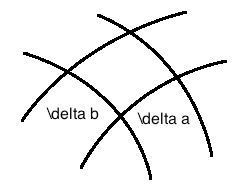
\includegraphics[width=0.3\textwidth]{images/quadrilateral.png}
\caption{A quadrilateral in curved space}
\end{figure}

\begin{align}
R^{\alpha}_{\beta\mu\nu}&=2\times\text{Christoffel 1st derivative}+ 2\times \text{products of Christoffel}\\
&=\Gamma^{\alpha}_{\beta\mu,\nu}-\Gamma^{\alpha}_{\beta\nu,\mu}
-\Gamma^{\alpha}_{\lambda\nu}\Gamma^{\lambda}_{\beta\nu}
+\Gamma^{\alpha}_{\lambda\nu}\Gamma^{\lambda}_{\beta\mu}
\end{align}


\subsubsection{Symmetrics of the Riemann tensor}
\begin{equation}
R_{\alpha\beta\mu\nu}=g_{\alpha\lambda} R^{\lambda}_{\beta\nu\mu}
\end{equation}
\begin{itemize}
\item $R_{\alpha\beta\mu\nu}$ is antisymmetric in $\mu\leftrightarrow\nu$ (see picture; this is eqivalent to circumnavigating the loop in opposit direction)
\item $R_{\alpha\beta\mu\nu}$ is antisymmetric in $\alpha\leftrightarrow \beta$
\item $R_{\alpha\beta\mu\nu}$ is symmetric under exchange of pairs; i.e. $R_{\alpha\beta\mu\nu}=R_{\mu\nu\alpha\beta}$
\item ``Symmetric'' under cyclic permutation of last three indices (Jordan symmetry)
\begin{equation}
0=R_{\alpha\beta\mu\nu}+R_{\alpha \mu \nu \beta} + R_{\alpha \nu \beta \mu}
\end{equation}
\end{itemize}

After applying these symmetrics to the $4\times 4 \times 4 \times 4=256$ components of the Riemann tensor, we reduce them down to only 20.


\underline{Proof}: go into local Minkowski coordinates (i.e. flat patch). Here $\Gamma$'s are zero, but their derivatives are not.

\begin{equation}
R_{\alpha\beta\mu \nu}=\Gamma^{\alpha}_{\beta \mu , \nu} - \Gamma^{\alpha}_{\beta \nu , \mu}
\end{equation}
Substitute
\begin{equation}
\Gamma^{\alpha}_{\beta \mu}=\frac{1}{2}g^{\alpha \lambda}\left(g_{\lambda \beta, \mu} + g_{\lambda \mu, \beta} 
- g_{\beta\mu , \lambda}\right)
\end{equation}
We lower the indices by
\begin{equation}
R_{\alpha \beta \mu \nu} = g_{\alpha\sigma} R^{\sigma}_{\beta \mu \nu}
\end{equation}
We now derivates with respect to $\nu$ (as an exercise)

\begin{equation}
\Rightarrow R_{\alpha\beta\mu\nu}=\frac{1}{2}\left(g_{\alpha \nu, \beta \mu} + g_{\beta \mu,\alpha \nu}
-g_{\alpha \mu, \beta \nu} - g_{\beta \nu, \alpha \mu}\right)
\end{equation}

Let's start with last symmetry (12 terms).

\begin{equation}
R_{\alpha \beta \mu \nu} + R_{\alpha \mu \nu \beta} + R_{\alpha \nu \beta \mu} = \text{12 terms}
\end{equation}
\exercise{Check that these terms cancel pairwise.}{}

\begin{equation}
R_{\alpha \beta \mu \nu} + R_{\alpha \mu \nu \beta} + R_{\alpha \nu \beta \mu} = 0.
\end{equation}
which is derived in local falt. But it's a perfectly good tensor equation $\Rightarrow$ it is coordinate independent $\Rightarrow$ true in curved space, also.

A good tensor equation = something built out of tensors $\pmx{M\\N}$ (which transform like they should) using valid operations like outer product, symmetrisation etc.

An example of a bad tensor equation:
\begin{equation}
R_{\alpha \beta \mu \nu , \lambda}=0
\end{equation}
because ordinary derivatives \textbf{,} are ``not good''; however
\begin{equation}
R_{\alpha \beta \mu \nu ; \lambda}=0
\end{equation}
is a good tensor equation, since covariant derivatives \textbf{;} are ``good''.


\subsection{Constructing new tensors from Riemann on the way to Einstein's field equations}
Aside: Riemann as a commutator
\begin{equation}
(V^{\mu}_{j\alpha})_{;\beta}-(V^{\mu}_{j\beta})_{;\alpha}=R^{\mu}_{\nu\alpha\beta}V^{\nu}
\end{equation}
This is a good tensor equation: it is true in all reference frames.

Aim:
\begin{itemize}
\item Derive Bianchi identities, which contain infofrmation about symmetries of Riemann tensor's derivatives
\item Contract Riemann in the hope of making a smaller tensor with 10 independent stress-energy tensor components, to match the 10 independent stress-energy components $T^{\mu\nu}$
\item Combine the above 2 aims to ``derive'' Einstein's field equations in the form 
\begin{equation}
(\text{curvature})=(\text{stress energy})
\end{equation} 
\end{itemize}

Bianchi identities
\begin{equation}
R_{\alpha\beta\mu\nu}=\frac{1}{2}\left(g_{\alpha\nu,\beta\mu}+g_{\beta\mu,\alpha\nu}-g_{\alpha\mu,\beta\nu}
-g_{\beta\nu,\alpha\mu}\right)
\end{equation}
Note $R_{\alpha\beta\mu\nu}$ is antisymmetric under exchange $\alpha\leftrightarrow \beta$ and $\mu \leftrightarrow \nu$, and under $\alpha \beta \leftrightarrow \mu \nu$.

We differentiate with respect to $x^{\lambda}$ and add
\begin{equation}
R_{\alpha\beta\mu\nu,\lambda}=\frac{1}{2}\left(g_{\alpha,\beta\mu\lambda}+g_{\beta\mu,\alpha\nu\lambda}
-g_{\alpha\mu,\beta\nu\lambda}-g_{\beta\nu,\alpha\mu\lambda}\right)
\end{equation}

Add cyclic permutations
\begin{equation}
R_{\alpha\beta\mu\nu,\lambda}+R_{\alpha\beta\nu\lambda,\mu}+R_{\alpha\beta\lambda\mu,\nu}=0
\end{equation}
(show this as an exercise)

Note that in flat space, $\Gamma$'s are zero. So,
\begin{align}
R_{\alpha\beta\mu\nu,\lambda}&=R_{\alpha\beta\mu\nu,\lambda}
+\overbrace{\Gamma\text{'s}\times R}_{\text{correct for each index}}\\
&=R_{\alpha\beta\mu\nu;\lambda},\quad\text{since $\Gamma$'s are zero}
\end{align}

Now we have a new good tensor equation valid in all coordinate systems.

\begin{equation}
0=R_{\alpha\beta\mu\nu;\lambda}+R_{\alpha\beta\nu\lambda;\mu}+R_{\alpha\beta\lambda\mu;\nu}
\end{equation}
the Bianchi identity!

How does the field evolve due to a source? (; is coordinate independent)

Note: need derivatives of curvature is we hope to describe how curvature evolves in response to source $T^{\mu\nu}$ (and how it evolves).

\subsubsection{Contractions of Riemann}
How many independent ways can we do this? $R^{\nu}_{\beta\mu\nu}$
\begin{align}
\Rightarrow R^{\alpha}_{\alpha\mu\nu}&=\underbrace{g^{\alpha\lambda}}_{\text{sym }\alpha\leftrightarrow\lambda} \overbrace{R_{\lambda\alpha\mu\nu}}^{\text{anti-sym }\lambda\leftrightarrow\alpha}\\
&=-g^{\lambda\alpha} R_{\alpha\lambda\mu\nu}\\
&=-R^{\lambda}_{\lambda\mu\nu}\\
&=0
\intertext{}
R^{\alpha}_{\beta\alpha\nu}&=?\\
R^{\alpha}_{\beta\mu\alpha}&=g^{\alpha\lambda} R_{\lambda\beta\mu\alpha}\\
&=-g^{\alpha\lambda} R_{\lambda\beta\alpha\mu}\\
&=-R^{\alpha}_{\beta\alpha\mu}\\
&=-R^{\alpha}_{\beta\alpha\nu}
\end{align}
(exercise: check the others)

The only independent contraction:
\begin{equation}
R_{\beta\nu}=R^{\alpha}_{\beta\alpha\nu}
\end{equation}

Ricci tensor is symmetric!
\begin{align}
R_{\nu\beta}=R^{\alpha}_{\nu\alpha\beta}&=g^{\alpha\lambda} R_{\lambda\nu\alpha\beta}\\
&=g^{\alpha\lambda} R_{\alpha\beta\lambda\nu}\\
&=R^{\lambda}_{\beta\lambda\nu}\\
&=R_{\beta\nu}
\end{align}


We can derive the Bianchi identities for the Ricci tensor from the Riemann tensor.

\begin{align}
0&=R_{\alpha \beta\mu\nu;\lambda}+R_{\alpha\beta\nu\lambda;\mu}+R_{\alpha\beta\lambda\mu;\nu}
\intertext{Raise 1st index by contracting with metric (also $\nabla g = 0$). Contract $\alpha$ with $\mu$}
0&=\underbrace{R^{\alpha}_{\beta\alpha\nu;\lambda}}_{R_{\beta\nu;\lambda}}+R^{\alpha}_{\beta\nu\lambda;\alpha}+
\underbrace{R^{\alpha}_{\beta\lambda\alpha;\nu}}_{-R^{\alpha}_{\beta\alpha\lambda;\nu}=-R_{\beta\lambda;\nu}}\\
0&=R_{\beta\nu;\lambda} + R^{\alpha}_{\beta\nu\lambda;\alpha} - R_{\beta \lambda ; \nu}
\end{align}

We contract again (involves Ricci scalar)

\begin{equation}
R = R^{\beta}_{\beta}=g^{\beta\nu}R_{\beta\nu}
\end{equation}

Contract Bianchi: raise $\beta$ and contract with $\nu$ (use $\nabla g = 0$).
\begin{equation}
0=\underbrace{R^{\beta}_{\beta;\lambda}}_{R_{;\lambda}}
+\underbrace{R^{\alpha\beta}_{\beta\lambda;\alpha}}_{-R^{\beta\alpha}_{\beta\lambda;\alpha}=-R^{\alpha}_{\lambda;\alpha}}
- R^{\beta}_{\lambda;\beta}
\end{equation}
(note we have skipped a few steps to get to this point, incl. raising $\beta$)
where $R_{;\lambda}$ is the Ricci scalar. It is important to remember that the antisymmetry properties of Riemann are only immediately true in the case where all indices are down; we cannot immediately say the second term has the antisymmetry shown (though it can be shown that it indeed does).
\begin{align}
\text{i.e. } 0&=R_{;\lambda}-2R^{\beta}_{\lambda;\beta}
\intertext{We play with this to get it into the form $(\ldots)_{;\beta}=0$}
0&=\left(R \delta ^{\beta}_{\lambda} - 2R^{\beta}_{\lambda}\right)_{;\beta}
\end{align}
We define the Einstein curvature tensor
\begin{align}
G^{\beta\lambda}&\equiv R^{\beta\lambda}-\frac{1}{2}R g^{\beta\lambda}
\intertext{Note this is just pretty notation, nothing exciting. Then,}
G^{\beta}_{\lambda}&=R^{\beta}_{\lambda}-\frac{1}{2}R g^{\beta}_{\lambda}=\delta^{\beta}_{\lambda}
\intertext{So we have that}
G^{\beta}_{\lambda;\beta}&=0
\end{align}
The diveregence of the Einstein curvature tensor vanishes!

\subsection{Einstein's field equations}
These cannot be derived; they are experimental laws. We shall motivate them heuristically.

\begin{enumerate}
\item Equivalence principle $\Rightarrow$ make sure our field equations are good tensor equations
\item In the weak field, we must recover Newtonian gravity
\begin{equation}
\nabla^2 \Phi = 4\pi G\rho
\end{equation}
\item Weak field suggests 2nd derivative of field (analogy: $g_{\mu\nu}$) proportional to energy density ($\rho c^2$)
\begin{itemize}
\item i.e., curvature (2nd derivatives of metric) $\propto T^{\mu\nu}$ (stress-energy tensor)
\end{itemize}
\item $T^{\mu\nu}$ has 10 independent components. \\What curvature quantity matches this? Ricci (for example)! So should we postulate $R^{\mu\nu}\propto T^{\mu\nu}$?
\item No! It violates energy conservation. We must have $T^{\mu\nu}_{;\nu}=0$. But then 
\begin{align}
R^{\mu\nu}_{;\nu}&=-\text{Ricci scalar}\\
&\neq 0 \text{ in general}
\end{align}
\item But we do have a nice curvature-related $\pmx{0\\2}$ tensor (or $\pmx{2\\0}$) whose divergence is zero, namely $G^{\beta\lambda}$. So we postulate
\begin{equation}
G^{\beta\lambda}\propto T^{\beta\lambda}
\end{equation}
\end{enumerate}
In fact we can be a tiny bit more general and ask: what symmetric tensor can we construct from Ricci and the metric on LHS?
\begin{equation}
R^{\alpha\beta}+\mu R g^{\alpha\beta} + \Lambda g^{\alpha\beta}=kT^{\alpha\beta}
\end{equation}
\begin{enumerate}
\item Insist on $T^{\alpha\beta}_{;\beta}=0$\\$\Rightarrow \mu = -\frac{1}{2}$ as calculated above
\item Insist on $\nabla^2=4\pi G\rho$ in weak field (which we will prove later)
\begin{equation}
\Rightarrow k = 8\pi G = 8\pi\text{ in natural units}
\end{equation}
\end{enumerate}

Einstein's field equations:
\begin{equation}
\underbrace{R^{\alpha\beta}-\frac{1}{2} R g^{\alpha\beta}}_{G^{\alpha\beta}}+\Lambda g^{\alpha\beta} = 8\pi T^{\alpha\beta}
\end{equation}
where $\Lambda$ is the ``cosmological'' constant (air-quotes because we do not need to discuss it in a cosmological context). This term is sometimes missing from t-shirts.

This can also be written with indices down, as
\begin{equation}
\underbrace{R_{\alpha\beta}}_{\mathclap{\text{Ricci tensor}}}
-\frac{1}{2} \overbrace{R}^{\mathclap{\text{Ricci scalar}}} g_{\alpha\beta}
+\underbrace{\Lambda g_{\alpha\beta}}_{\mathclap{\text{cosmological constant}}} = 8\pi T_{\alpha\beta}
\end{equation}


\pagebreak

\part{Terrestrial and astronomical applications}

Today we will discuss:
\begin{itemize}
\item what is $T_{\mu\nu}$?
\item where did the 10 ``missing'' curvature degrees of freedom go?
\end{itemize}

\section{Stress energy}
The principle of equivalence says we work out $T$ as a tensor in Minkowski space $\Rightarrow$ same tensor form in curved space. This is true for all geometric objects (when a new piece of phyiscs is introduced, we refer back to local flat space, because this is all we can do).

Components:
\begin{align}
&&&\text{e.g. EM}\nonumber \\
T^{00}&=\text{energy density}\equiv\text{energy/volume}&&\frac{1}{2}\epsilon_0 E^2 + \frac{B^2}{2\mu_0}\\
T^{0i}&=\text{energy flux}\equiv\text{energy/area/time}&&\frac{(\vect{E} \times \vect{B})_i}{\mu_0}\\
T^{ij}&=\text{momentum flux}&&\epsilon_0 E_i E_j 
+ \frac{1}{\mu_0}-\left(\frac{1}{2}\epsilon_0 E^2+\frac{B^2}{2\mu_0}\right)\delta_{ij}
\end{align}

$T^{ij}$ is momentum/area/time in $i$th direction transported through area defined by normal along $j$ direction.

It is easy (as an exercise; see textbooks) to write $T$ in Minkowski coordinates as a tensor equation involving the Faraday tensor 
$F_{\mu\nu} = \partial_\mu A_{\nu}-\partial_{\nu}A_{\mu}$. Then this is true in curved space too.

For particles:
\begin{itemize}
\item ``cold dust'': at temperature $=0$, all particles in local volume have a single bulk velocity
\item perfect fluid/gas: particles have bulk motion plus random motions, i.e. pressure
\end{itemize}

\example{?}{
Considering dust,
\begin{equation}
T^{00}\sim \rho c^2,\quad T^{0i}\sim \rho v^{i}, \quad T^{ij}\sim \rho v^{i} v^{j}\quad \text{(heuristically)}
\end{equation}
Formally, we can do this by letting $n_0=$ proper number density (in fluid bulk frame). 

Then define a particle flux 4-vector $\vec{N}=n_0\vec{u}$. 

Note that divergence of $\vec{N}$ vanishes by particle conservation.

Then $T=\vec{p} \otimes \vec{N}$ where $\vec{p}$ is the bulk momentum.

If we consider a single species of aprticle, with mass $m$ and proper density $n_0$,
\begin{equation}
T=m\vec{u}\otimes n_0\vec{u}
\end{equation}
with components
\begin{equation}
T^{\mu\nu}=m n_0 u^{\mu} u^{\nu}
\end{equation}
}

\example{?}{
We now consider a perfect fluid.

Each particle (label it $A$) has 4-velocity
\begin{equation}
\vec{w}_A=\underbrace{\vec{u}_A}_{\mathclap{\text{organised bulk}}}
+\overbrace{\delta \vec{u}_A}^{\mathclap{\text{random}}}
\end{equation}

For the total fluid, we sum over the particle (i.e. take the average)
\begin{align}
T&=\sum_A m n_0 \left(\vec{u}_A \otimes \vec{u}_A 
+ \underbrace{2\vec{u}_a \times \delta \vec{u}_A}_{\mathclap{\approx0~\text{(random vector $\delta\vec{u}_A$)}}}
+ \overbrace{\delta \vec{u}_A \times \delta \vec{u}_A}^{\text{pressure}}\right) \label{random motion} \\
&= p g + (\rho + p)~\vec{u} \otimes \underbrace{\vec{u}}_{\mathclap{\text{bulk 4-velocity}}}
\end{align}


where $\rho$ is the mass density. Note that in~(\ref{random motion}) the sum over the random vector will go to zero, as it averages to zero.

If there is no bulk motion then (Minkowski) $\vec{u}=(1,0,0,0)$
\begin{align}
T^{00}&=p g^{00}+(\rho+p)\cdot 1 &&= \rho,\quad\text{rest energy density}\\
T^{11}&=pg^{11}+(\rho+p)\cdot \underbrace{u^{1} u^{1}}_{0} &&=p,
\quad\underbrace{\text{isotropic pressure}}_{T^{11}=T^{22}=T^{33}}
\end{align}

Note that this section relates to Schutz Chapter 4; we should read it carefully and do some of the problems (also relating to assignment 3).
}

\section{Gauges}


We work towards a weak-field theory, which we need to treat solar system/terrestrial experiments (see earlier sections).

The Einstein field equations are 10 indepedent equations when viewed in isolation. But we know there are \underline{4} degrees of freedom which we know \underline{physically} to be dependent, because we can always choose 4 coordinates, i.e. 4 gauge choices, as we please (no matter how complicated $T$ is).

$\therefore$ 6 truly independent field equations. We can compare this to electromagnetism (EM):
\begin{itemize}
\item 6 field variables $\vect{E}$, $\vect{B}$
\item these reduce to 4 potentials $\Phi$, $\vect{A}$
\item these reduce further to 3 equations via gauge choices
\end{itemize}

Recall in EM:
Faraday field tensor (we will work in flat space)
\begin{align}
F_{\mu\nu}&=\partial_{\mu} A_{\nu} - \partial_{\nu} A_{\mu}\\
\text{Let } \bar{A}_{\nu}&=A_{\nu}+\partial_{\nu} \chi,\quad\text{where $\chi$ is an arbitrary scalar function}\\
\bar{F}_{\mu\nu}&=\partial_\mu \bar{A}_\nu - \partial_\nu \bar{A}_\mu\\
&= F_{\mu\nu}+\partial_\mu \partial_\nu \chi - \partial_\nu \partial_\mu \chi\\
&=F_{\mu\nu}
\end{align}
i.e. Faraday tensor is unchanged under gauge transformation (as an exercise, show that this is also true in curved space).

Furthermore in flat space, the homogeneous Maxwell equations read
\begin{equation}
0=F_{\mu\nu,\alpha}+F_{\nu\alpha,\mu} + F_{\alpha\mu,\nu}
\end{equation}
and all the Christoffels are zero, so we can add zeroes to the RHS of the above equation to get in curved space
\begin{equation}
 0=F_{\mu\nu;\alpha}+F_{\nu\alpha;\mu} + F_{\alpha\mu;\nu}
\end{equation}

This is of an identical form to the Bianchi identities (satisfied by the Riemann tensor in GR which is slightly larger; here it is satisfied by the Faraday tensor).

\begin{enumerate}
\item In EM, Biachi tells us we can write $\vect{E}$ and $\vect{B}$ in terms of $\vect{A}$ and $\Phi$ (via $\div \vect{B}=0$ + Faraday's law). Likewise, in GR Bianchi tells us $R_{\alpha\beta\gamma\delta}$ can be written in terms of ``potentials'' (see below).

\item By analogy with EM Bianchi, it is clear that GR also has an ``electric'' and ``magnetic'' subdivision of the metric satisfying the generalised Faraday's law. We often see talk of gravitoelectric and gravitomagnetic effects (even when $F^{\mu\nu}=0$; i.e. when there are no electric and magnetic fields - these are not actually caused by EM, but rather appear analogously)
\end{enumerate}

An example of a gravitomagnetic effect is Lense-Thirring precession.

What are the ``potentials'' in GR? Unfortunately it is not as simple as saying
\begin{equation}
R_{\alpha \beta \gamma \delta}= A_{\beta \gamma\delta;\alpha} - A_{\alpha \beta \gamma ; \delta},\quad\text{for some
$A_{\alpha\beta\gamma}$}\nonumber
\end{equation}

This is clearly not true - the symmetry and anti-symmetry of the indices leads either to trivialities or contradictions

Luckily our maths \cancel{friends} frenemies :) have shown that there exists Ricci decomposition for Riemann
\begin{align}
R_{\alpha\beta\gamma\delta}&=\frac{R}{6}\underbrace{g_{\alpha[\gamma}g_{\delta]\beta}}_{\text{scalar}}
+\underbrace{g_{\alpha[\gamma} S_{\delta]\beta}- g_{\beta[\gamma} S_{\delta]\alpha}}_{\text{semi-traceless}}
 + \underbrace{C_{\alpha\beta\gamma\delta}}_{\text{traceless}}
\intertext{}
\text{where }[\ldots]&=\text{antisymmetrisation}\\
S_{\alpha\beta}&=R_{\alpha\beta}-\frac{1}{4}R g_{\alpha\beta}\\
C_{\alpha\beta\gamma\delta}&=\text{Weyl tensor}
\end{align} 

See footnote for antisymmetrisation\footnote{
$g_{\alpha[\gamma}g_{\delta]\beta} = g_{\alpha\gamma}g_{\delta\beta} - g_{\alpha\delta}g_{\gamma \beta}$}

The Weyl tensor is a complicated thing involving derivatives of Lanczos tensor $H_{\alpha\beta\gamma}$; it is where the 10 ``missing'' degrees of freedom in Riemann went, i.e. the ones \underline{not} in Eintein's field equation.

The Einstein field equations involve the trace of Riemann (to get the Ricci tensor), and since $C_{\alpha\beta\gamma\delta}$ is traceless and hence disappears (does not appear in the field equations.

Equation of motion for Weyl:
\begin{equation}
C_{\alpha\beta\gamma\phantom{\delta};\delta}^{\phantom{\alpha\beta\gamma}\delta}=\text{stuff involving $R_{\beta\nu}$ and its covariant}
\end{equation}
By analogy, the EM inhomogeneous Maxwell:
\begin{equation}
F^{\mu\nu}_{\phantom{\mu\nu};\nu}=\mu_0 J^{\mu}
\end{equation}

GR case: invariant under gauge transform
\begin{equation}
\bar{H}_{\alpha\beta\gamma}=H_{\alpha\beta\gamma}+\chi_{[\alpha}g_{\beta]\gamma}
\end{equation}
where $\chi_{\alpha}$ is an arbitrary 1-form (4 functions because we are free to make 4 coordinate choices)

Nice gauge choices:
\begin{itemize}
\item algebraic
\begin{equation}
3\chi_{\alpha}=H_{\alpha\phantom{\beta}\beta}^{\phantom{\alpha}\beta}
\end{equation}
\item differential (like Lorenz in EM, $A^{\mu}_{\phantom{\mu};\mu}=0$)
\begin{equation}
H_{\alpha\beta\phantom{\gamma};\gamma}^{\phantom{\alpha\beta}\gamma}=0
\end{equation}
\end{itemize}

\subsection{Weak fields}
Spacetime is nearly flat
\begin{align}
g_{\mu\nu}&=\underbrace{\eta_{\mu\nu}}_{\mathclap{\text{Minkowski}}} + h_{\mu\nu}
\intertext{with}
\lvert h_{\mu\nu} \rvert &\ll 1\quad\text{(this is element-wise comparison)}
\end{align}

This implies a restricted choice of coordinates, e.g. spherical polars are \underline{not} appropriate ($r,\theta$, etc.)

We define and use two kinds of transformations. Our aim is to find a metric suitable for terrestrial and solar system applcations, e.g. Pound-Rekba experiment.

\subsubsection{Background Lorentz transformations}
\begin{equation}
dx^{\bar{\alpha}}=\Lambda^{\bar{\alpha}}_{\phantom{\alpha}\beta}dx^{\beta}
\end{equation}
from special relativity with reference to a flat background. Applying this to the metric:
\begin{align}
g_{\bar{\alpha}\bar{\beta}}&=\Lambda^{\alpha}_{\phantom{\alpha}\bar{\alpha}} 
\Lambda^{\beta}_{\phantom{\beta}\bar{\beta}} \left(\eta_{\alpha\beta}+h_{\alpha\beta}\right)\\
&=\eta_{\bar{\alpha}\bar{\beta}}+h_{\bar{\alpha}\bar{\beta}},\quad\text{by definition}
\end{align}
where $h_{\bar{\alpha}\bar{\beta}}$ means ``via background Lorentz''.

\subsubsection{Gauge transformation: small coordinate change}

The gauge transformation we use is:

\begin{equation}
\vec{x} \mapsto \vec{x} + \underbrace{\vec{\xi}(\vec{x})}_{\text{small}}
\end{equation}
By small we mean $\lvert \xi \rvert \ll \lvert \vec{x} \rvert$.

The transform matrix is then
\begin{equation}
x^{\alpha} \mapsto x^{\alpha'} = x^{\alpha} + \underbrace{\xi^{\alpha}(\vec{x})}_{\text{small}}
\end{equation}
where ``small'' is as previous, though evaluated element-wise.

So now, our metric in primed coordinates is:

\begin{align}
g_{\alpha'\beta'}&=\Lambda^{\alpha}_{\phantom{\alpha}\alpha'} \Lambda^{\beta}_{\phantom{\beta}\beta'}
(\eta_{\alpha\beta}+h_{\alpha\beta})\\
&=\delta^{\alpha}_{\phantom{\alpha}\alpha'}\delta^{\beta}_{\phantom{\beta}\beta'}\eta_{\alpha\beta}
-\frac{\partial \xi^{\alpha}}{\partial x^{\alpha'}} \delta^{\beta}_{\phantom{\beta}\beta'}\eta_{\alpha \beta}
-\delta^{\alpha}_{\phantom{\alpha}\alpha'}\frac{\partial \xi^{\beta}}{\partial x^{\beta'}}\eta_{\alpha\beta}
+\delta^{\alpha}_{\phantom{\alpha}\alpha'}\delta^{\beta}_{\phantom{\beta}\beta'}h_{\alpha\beta}
+\text{2nd order corrections}\\
&=\eta_{\alpha'\beta'}-\xi_{\beta', \alpha'}-\xi_{\alpha', \beta'}+h_{\alpha'\beta'}
\end{align}
where $\xi_{\beta'}=\eta_{\beta'\gamma'}\xi^{\gamma'}$, i.e. all raising and lowering is done with Minkowski metric.

This is like an EM gauge transform, cf. $A_{\mu}\mapsto A_{\mu}+\frac{\partial \chi}{\partial x^{\mu}}$ except that our
$\vec{\xi}$ has 4 degrees of freedom, \underline{not} one (physically: we are free to choose 4 coordinates).

We can now calculate Christoffel symbols, Riemann tensor etc. from this metric. Algebra is left as an exercise.

\begin{equation}
R_{\alpha\beta\mu\nu}=g_{\alpha \lambda} R^{\lambda}_{\phantom{\lambda}\beta\mu\nu}
=\frac{1}{2}\left(h_{\alpha\nu,\beta\nu}+h_{\beta\mu,\alpha\nu}-h_{\alpha\mu,\beta,nu}-h_{\beta\nu,\alpha,mu}\right)
\end{equation}
noting that the derivatives of $\eta$ vanishes.

\exercise{We can check that $R$ is invariant under gauge transform
\begin{equation}
\bar{h}_{\alpha\nu}=h_{\alpha\nu}-\xi_{\alpha,\nu}-\xi_{\nu,\alpha}
\end{equation}

We will get lots of pairwise cancellation because $\xi_{\alpha,\beta \gamma\delta}$ is the same for all perumtations of $\{\beta,\gamma,\delta\}$. We can choose $\vec{\xi}$ cleverly to simplify.
}
{}

Considering the Ricci tensor,
\begin{equation}
R_{\beta\nu}=g^{\alpha\lambda} \underbrace{R_{\lambda\beta\alpha\nu}}_{\mathclap{\text{1st order only}}}
\cong \eta^{\alpha\lambda} R_{\lambda\beta\alpha\nu},\quad\text{to 1st order}
\end{equation}
The Ricci scalar:
\begin{equation}
R = g^{\beta\nu} \underbrace{R_{\beta\nu}}_{\mathclap{\text{also 1st order}}} \cong \eta^{\beta\nu} R_{\beta\nu}+
\text{quadratic bits}
\end{equation}

Collect eveerything in Einstein tensor:
\begin{equation}
G_{\beta\nu}=R_{\beta\nu}-\frac{1}{2}R g_{\beta\nu}
\end{equation}
The algebra is left as an exercise, but we get
\begin{align}
G_{\beta\nu}=&~\frac{1}{2}\left(h^{\alpha}_{\phantom{\alpha}\nu,\beta\alpha}+h_{\beta\alpha,\phantom{\alpha}\nu}
^{\phantom{\beta\alpha,}\alpha} - h^{\alpha}_{\phantom{\alpha}\alpha,\beta\nu}- h_{\beta\nu,\phantom{\alpha}\alpha}
^{\phantom{\beta\nu,}\alpha}\right)\\
&-\frac{1}{2}\eta_{\beta\nu}
\left( h^{\alpha\phantom{\lambda}\lambda}_{\phantom{\alpha}\lambda,\phantom{\lambda,}\alpha}
- h^{\lambda\phantom{\lambda,}\alpha}_{\phantom{\lambda}\lambda,\phantom{\alpha}\alpha}\right)
\end{align}
Note, all raising and lowering is done with Minkowski metric.
\begin{align}
\text{e.g. } h^{\alpha}_{\phantom{\alpha}\nu,\beta\alpha}&
=\eta^{\alpha\mu}\frac{\partial h_{\mu\nu}}{\partial x^{\beta}\partial x^{\alpha}}\\
h_{\beta\alpha,\phantom{\alpha}\nu}^{\phantom{\beta\alpha,}\alpha}&=
\frac{\partial h_{\beta\alpha}}{\partial x^{\mu} \partial x^{\nu}}\eta^{\alpha\mu}\quad\text{etc.}
\end{align}

Terms (2nd derivatives, since curvature) are mainly of the form 
\begin{align}
&(\underbrace{h_{\alpha \beta,}^{\phantom{\alpha\beta,}\alpha}}_{\mathclap{\div h}})_{,\text{ something}}\\
\text{or }=& (\underbrace{h^{\alpha}_{\phantom{\alpha}}}_{\mathclap{\text{trace of $h$}}})_{,\text{ two somethings}}
\end{align}

This suggests a good gauge choice is something traceless and divergenceless (like Lorenz gauge in EM, divergenceless).

We define a trace-reveresed metric
\begin{equation}
\bar{h}_{\beta\nu}=h_{\beta\nu}-\frac{1}{2}\eta_{\beta\nu}h^{\lambda}_{\phantom{\lambda}}
\end{equation}
Also impose the gauge condition
\begin{equation}
\bar{h}_{\beta\nu,}^{\phantom{\beta\nu,}\nu}=0\quad\text{(Lorenz)}
\end{equation}

Substitute (as an exercise)
\begin{equation}
G_{\beta\nu}=-\frac{1}{2}\Box \bar{h}_{\beta\nu}
\end{equation}
where $\Box$ is the D'Alembertian in flat space
\begin{equation}
\Box = \frac{\partial^2}{\partial t^2}+\nabla^2
\end{equation}

Einstein equation without cosmological constant is
\begin{equation}
\Box \bar{h}_{\mu\nu}=-16 \pi T_{\mu\nu},\quad\text{weak field}
\end{equation}

This is a wave equation wih source on RHS.

\review{Recall, in the weak field limit we express the metric as
\begin{equation}
g_{\mu\nu}=\eta_{\mu \nu}+h_{\mu \nu}
\end{equation}
where $h_{\mu\nu}$ is small. The trace-reversed version of $h$ is
\begin{equation}
\bar{h}_{\mu\nu}=h_{\mu\nu}-\frac{1}{2}\eta_{\mu\nu}h^{\lambda}_{\phantom{\lambda}\lambda}
\end{equation}
We choose our gauge so that
\begin{equation}
h_{\mu\nu,}^{\phantom{\mu\nu,}\nu}=0
\end{equation}
which is the Lorenz gauge. From this we get a wave equation,
\begin{equation}
\Box \bar{h}_{\mu\nu}=-16\pi T_{\mu\nu}\label{wave eqn}
\end{equation}
}

\section{Applications of Einstein's Field Equations}
We will consider how we can apply the wave equation~(\ref{wave eqn}) to terrestrial situations (e.g. gravity on Earth).

To do this, we will have to neglect many components! (this is since we do not actually need 10 separate equations to describe, for example, the motion of a tennis ball).

\subsection{Perfect fluid}

For a perfect fluid, $T_{\mu\nu}=p g_{\mu\nu}+(p+\rho)u_{\mu} u_{\nu}$, so
\begin{align}
T_{00}&\sim \rho\\
T_{0i}&\sim \rho\times \text{velocity}\\
T_{ij}&\sim \rho\times\text{(velocity)}^2
\end{align}
where the last two are $\ll \rho$ if the velocity of the source is $\ll c$.

Consider only
\begin{align}
\Box \bar{h}_{00}&=-16\pi T_{00}=-16\pi\rho
\intertext{where}
\Box &=-\frac{\partial^2}{\partial t^2}+\nabla^2\approx \nabla^2
\intertext{because we want static gravity, not a wave}
\end{align}
Alternatively, 
\begin{equation}
\frac{\partial / \partial t}{\nabla}\sim\frac{\text{length}}{\text{time}}\sim\text{velocity}\ll 1
\end{equation}
\begin{equation}
\text{i.e., } \nabla^2 \bar{h}_{00}=-16\pi \rho
\end{equation}

In the Newtonian limit (experimental):
\begin{equation}
\nabla^2 \Phi = 4\pi \underbrace{G}_{\mathclap{\text{we will set $G=1$}}} \rho
\end{equation}
That is,
\begin{equation}
\bar{h}_{00}=-4 \underbrace{\Phi}_{\mathclap{\text{Newtonian gravitational potential}}}
\end{equation}
and other $\bar{h}_{\mu\nu}$'s are tiny.

Going back to the original metric involving $h_{\mu\nu}$:
\begin{align}
h_{00}&=\bar{h}_{00}+\frac{1}{2}\eta_{00} h^{\lambda}_{\phantom{\lambda}\lambda}\\
&=\bar{h}_{00}+\frac{1}{2}\underbrace{\eta_{00}}_{-1}\underbrace{\eta^{\lambda\alpha}}
_{\mathrlap{-1 \text{ for }\lambda=\alpha=0}} \overbrace{h_{\lambda\alpha}}
^{\mathclap{\text{only significant for }\lambda=0,\alpha=0}}
\end{align}
NOTE: these is a minor error in the algebra above, according to Melatos.

\begin{align}
\text{i.e., } h_{00}&=\frac{1}{2}\bar{h}_{00}\\
&=-2\Phi
\end{align}
Similarly for $h_{11}$, etc. (trace $\neq 0$).

Put together we get the weak-field ``static'' metric:
\begin{equation}
g_{\mu\nu}=\diag (-1-2\Phi,1-2\Phi,1-2\Phi,1-2\Phi)
\end{equation}


\subsection{Pound-Rebka}

We consider the Pound-Rebka experiment (PUT FIGURE HERE). What is the photon frequency at the top/bottom of the tower?
\begin{align}
E_{\text{photon}}&=-\vec{u}\cdot \vec{p}\\
\vec{u}_{\text{top}}\cdot \vec{u}_{\text{top}}&=-1\\
g_{00}\left(u^0_{\text{top}}\right)^2&=-1\\
\text{i.e., } u^{0}_{\text{top}}&=\sqrt{1+2\Phi},\quad\text{$\Phi$ is small on Earth}\\
&\approx 1+\Phi\text{ (at top)}
\intertext{Simialrly stat. observation at bottom:}
u^0_{\text{bottom}}&=1+\Phi \text{ (at bottom)}
\end{align}

Also note that the metric is independent of time.

\begin{align}
\text{i.e., } p_0&=\text{constant}\\
E_{\text{top}}&=-u^0_{\text{top}}p_0\quad\text{and}\quad E_{\text{bottom}}
=-u^0_{\text{bottom}}p_0\\
\frac{E_{\text{top}}}{E_{\text{bottom}}}&=\frac{u^0_{\text{top}}}{u^0_{\text{bottom}}}
=\frac{1+\Phi\text{ (top)}}{1+\Phi\text{ (bottom)}}\approx 1+gH
\end{align}
where $H$ is the altitude difference, give $\Phi(z)=gz$.

\subsection{Gravity Probe B/Lense-Thirring precession}
L-T precession arises because inertial frames are dragged into rotation by a rotating object, e.g., a Kerr black hole!

Gravity Probe B is a test for precession of gyroscope (there are 4 probes) orbiting Earth ($\SI{650}{km}$ radius orbit). Launched in 2004-2005.

Two types of precession where measured:
\begin{itemize}
\item geodetic
\footnote{Gyroscope parallel transported in free fall, but space is curved by \underline{mass} of Earth (whether or not Earth rotates) $\Rightarrow$ spin doesn't return to original position} 
$6601\pm 18.3~\text{mas~yr}^{-1}$
\begin{itemize}
\item cf. 6606~mas~yr$^{-1}$ predicted from GR (where mas = milli-arcsecond)
\end{itemize}
\item Lense-Thirring
\footnote{We need Earth to rotate for Lense-Thirring precession. It is the angular momentum of Earth's contribution to $T^{\mu\nu}$}
: $37.2 \pm 7.2~\text{mas~yr}^{-1}$
\begin{itemize}
\item cf. 39.2~mas~yr$^{-1}$ predicted from GR
\end{itemize}
\end{itemize}
Beware stray electrostatic torques! This was an issue that took about a decade to work out.

Analysis:
\begin{enumerate}
\item What is gyroscope spin in geometric language?
\item How does Earth's mass \underline{and} rotation affect weak-field metric? (What we have done so far is not enough!)
\item How does spin evolve as it falls freely around Earth? (related to the geodesic equation)
\end{enumerate}

\subsection{Spin}
\begin{equation}
T^{\mu\nu}=\text{energy momentum tensor}
\end{equation}
Can we construct a geometric object containing angular momentum (AM) from $T^{\mu\nu}$? Recall 1st year:
\begin{equation}
\text{Angular momentum }I=\vect{x}\times \vect{p}
\end{equation}
We propose in GR that angular momentum is some osrt of vector and tensor. Specifically try
\begin{equation}
M^{\alpha\beta \gamma}=x^{\beta}T^{\gamma\alpha}-x^{\gamma}T^{\beta\alpha}
\end{equation}
Note this is antisymmetric in $\beta,\gamma$. Is it conserved?\footnote{We have local energy conservation, but there is energy and momentum in global curvature, etc.} Check divergence in local flatspace
\begin{align}
M^{\alpha\beta\gamma}_{\ph{\alpha\beta\gamma},\alpha}&=\delta^{\beta}_{\ph{\beta}\alpha}
T^{\gamma\alpha}+x^{\beta}\underbrace{T^{\gamma\alpha}_{\ph{\gamma\alpha},\alpha}}
_{\mathclap{=0\text{ because $\propto$ energy-momentum conversation}}}-\delta^{\gamma}_{\ph{\gamma}\alpha}T^{\beta\alpha}-
\underbrace{x^{\gamma}T^{\beta\alpha}}_{=0}\\
&=0\\
&=M^{\alpha\beta\gamma}_{\ph{\alpha\beta\gamma};\alpha}
\end{align}
hence this is also true in curved space.

Define
\begin{align}
J^{\beta\gamma}&=\int\text{d}^3\vect{x}~M^{0\beta\gamma}\\
\Rightarrow \frac{\text{d}J^{\beta\gamma}}{\text{d}t}&=\int \vect{d}^3\vect{x}~
\frac{\partial M^{0\beta\gamma}}{\partial t}\\
&=-\int \text{d}^3\vect{x}\frac{\partial M^{i\beta\gamma}}{\partial x^i}
\intertext{by conservation law, with $i=1,2,3$}
&=-\int \text{d}S~n_i M^{i\beta\gamma}
\end{align}
by Gauss' law.


Physically:
\begin{itemize}
\item $J^{0i}$ appears to depend on where you choose origin. We will ignore it.
\item $J^{ij}=\text{angular momentum}$, (e.g. $J^{12}$ is ``3'' component of AM)
\item $J^{\beta\gamma}$ is \underline{not} invariant under translation because it contains orbital AM.
\end{itemize}

We pull out just the spin:
\begin{equation}
S_{\alpha}=\frac{1}{2}\overbrace{\epsilon_{\alpha\beta\gamma\delta}}^{\mathclap{\text{Levi-Civita (anti-symmetric)}}}J^{\beta \gamma} \underbrace{u^{\delta}}_{\mathclap{4-\text{velocity}}}
\end{equation}

Check (as an exercise) physical meaning in components in MCRF (momentarily comoving reference frame) where $\vec{u}=(u^t,0,0,0)$
\begin{align}
S_0&=0\\
S_1&=J^{23}=\text{``1'' component of angular momentum}\\
\text{etc.}
\end{align}

Note: $S_{\alpha}u^{\alpha}=0$.

Step 2 $\to$ weak field metric (can also get as limit of Kerr BH solution, which we will see later)

Answer:

Post-Newtonian approximation
\begin{align}
\Gamma^{0}_{\ph{0}i0}\rvert_{\text{2nd order}}&=\frac{\partial \Phi}{\partial x^i}
\intertext{where $\Phi$ is the Newtonian potential.}
\Phi&=-\int \text{d}^3\vect{x}'~\frac{T^{00}\rvert_{\text{0th order}}}{|\vect{x}-\vect{x}'|}\\
\Gamma^{0}_{\ph{0}ij}\rvert_{\text{1st order}}&=0\\
\Gamma^{k}_{\ph{k}i0}\rvert_{\text{3rd order}}&=\frac{1}{2}\left(\frac{\partial \xi_i}
{\partial x^k}-\frac{\partial \xi^k}{\partial x^i}\right)-\delta^{k}_{\ph{k}i}\frac{\partial \Phi}
{\partial t}
\intertext{where}
\xi^i&=-4\int\text{d}^3\vect{x}'~\frac{T^{i0}\rvert_{\text{1st order}}}{|\vect{x}-\vect{x}'|}
\intertext{We get $T^{i0}\neq 0$ if rotating Earth, eg. $\propto M_{\text{Earth}}\cdot \text{rotational speed of Earth}\sim v^3$}
\Gamma^{k}_{\ph{k}ij}\rvert_{\text{2nd order}}&=-\delta_{ij}\Phi^{k}_{\ph{k},}
-\delta^{k}_{\ph{k}i}\Phi_{,j}+\delta^{k}_{\ph{k}j}\Phi_{,i}
\end{align}

These orders are ``leading order' for each Christoffel symbol (i.e. all lower orders are zero). Also note $i,j=\{1,2,3\}$.

So... we now use the metric.

What are the equations of motion of $S_{\alpha}$? We consider freefall: local Lorentz invariance then gives equations of motion of spin; $\vec{u}$ is the 4-velocity along the geodesic of freefall.

\begin{align}
0&=\nabla_{\vec{u}}\tilde{S}\\
u^{\beta} S_{\alpha;\beta}&=u^{\beta}\left(S_{\alpha,\beta}-\Gamma^{\lambda}_{\ph{\lambda}
\alpha\beta}S_{\lambda}u^{\beta}\right)
\end{align}

We want $\frac{dS_{\alpha}}{d\tau}$, i.e. how the $\tilde{S}$ changes along the geodesic parametrised by the proper time $\tau$.

We simplify: eliminate $S_0$ using $S_0 u^0 = -S_i u^i$ (see Weinberg for the algebra; we don't need to know the algebra, only the result).

To leading order, we can define a 3-vector
\begin{align}
\vect{L}&=(1+\Phi)\vect{S}-\frac{1}{2}\vect{v}(\vect{v}\cdot\vect{S})
\intertext{So we find}
\frac{d\vect{L}}{dt}&=\left(-\underbrace{\frac{1}{2}\nabla\times\vect{S}}_{\text{Lense-Thirring}}
-\frac{3}{2}\vect{v}\times \nabla\Phi \right)\times \vect{L}\label{dldt}
\end{align}
Geodetic $\vect{v}=\frac{d\vect{x}}{dt}$ where $\vect{v}$ is the 3-velocity of the spacecraft.

Precession! c.f.~(\ref{dldt}) with
\begin{equation}
\frac{d\vect{L}}{dt}=\vect{\Omega}_{\text{precession}}\times \vect{L}
\end{equation}

Geodesic happens because we are parallel transported around a closed loop.


\section{Gravitational waves}
There are 3 points to consider regarding grav. waves:
\begin{enumerate}
\item Propagation
\item Detection
\item Generation
\end{enumerate}

\subsection{Waves}
Some examples:
\begin{itemize}
\item \underline{Scalar}: sound (just need pressure, e.g. for space; or need density)
\item \underline{Vector}: photon in EM (two directions, need a vector)
\item \underline{Tensor}: grav. waves, elastic waves (displacements, not always same direction as force)
\end{itemize}

\underline{What do waves do?} They transport energy, momentum, angular momentum.
\begin{align}
\Rightarrow&\text{merging black holes}\Rightarrow\text{gravitational waves}\\
\Rightarrow&\text{rotating (off axis) magnet}
\end{align}

Waves are launched by a localised source.

\begin{figure}[h]
\centering
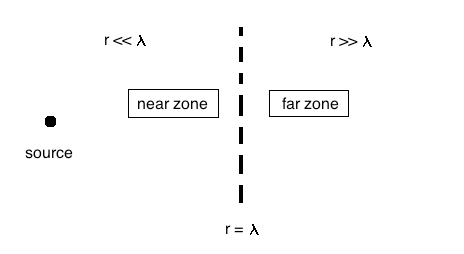
\includegraphics[width=0.7\textwidth]{images/waves-zones.png}
\caption{Near and far zones of a wave}
\end{figure}

In the near zone, waves $\sim$ quasi-static (static field source) $e^{-i\omega t}$. Usually steeper than $r^{-1}$, but $E_{\text{flux}}\propto r^{-2}$.

In far zone, we approximate a plane wave $\propto e^{i(kr-\omega t)}$; amplitude $\propto r^{-1}$, usually transverse energy $E \propto r^{-2}$.

In general in GR, we need non-linear analysis in the near zone.

\begin{align}
\text{Propagation}:&&~\underbrace{\Box\bar{h}_{\mu\nu}}_{\mathclap{\partial^\lambda \partial_{\lambda};\text{ raise/lower $\bar{\omega}$ Minkowski for linear waves}}}
&&=-16\pi T_{\mu\nu} = 0\quad\text{(in vacuum)}\\
\text{Plane wave solutions}:&&~\bar{h}_{\mu\nu}&&=A_{\mu\nu}e^{ik_{\alpha}x^{\alpha}}
\end{align}

\begin{align}
\Rightarrow \partial_{\lambda}\bar{h}_{\mu\nu}&=A_{\mu\nu}\partial_{\lambda}(ik_{\alpha}
x^{\alpha})e^{ik_{\alpha}x^{\alpha}}\\
&=A_{\mu\nu}ik_{\alpha}\delta^{\alpha}_{\ph{\alpha}\lambda}e^{ik_{\alpha}x^{\alpha}}\\
&=ik_{\lambda}\bar{h}_{\mu\nu}\\
\Box \bar{h}_{\mu\nu}&=-k^{\lambda}k_{\lambda}\bar{h}_{\mu\nu}=0\quad\text{(in vacuum)}
\end{align}

We have two possibilities:
\begin{itemize}
\item no wave ($\bar{h}_{\mu\nu}=0$)
\item $k^{\lambda}k_{\lambda}=0$, i.e. $\vec{k}$ null vector (or equivalently $\tilde{k}$ is a null 1-form)
\begin{itemize}
\item[] $d\tilde{\phi}=i\tilde{k}$
\end{itemize}
\end{itemize}

Local Minkowski:

\begin{equation}
\vec{k}=\left(\frac{\omega}{c},\vect{k}\right)\quad(c=1)
\end{equation}

i.e. $\omega^2 - |k|^2=0$ (use phase speed $=\frac{\omega}{k}=1$)

i.e. grav. waves propagate at $c=1$!

\begin{equation}
\Box \bar{h}=-16T\quad\text{in Lorentz (harmonic) gauge}
\end{equation}
Harmonic $\Rightarrow 0 =\bar{h}_{\mu\nu,}^{\ph{\mu\nu,}\nu}$; i.e. 
$\partial^{\nu}\bar{h}_{\mu\nu}=0$.

This implies a constraint on $A_{\mu\nu}$

Substitute in a plane wave,
\begin{equation}
0=ik^{\nu}A_{\mu\nu}e^{ik_{\alpha}x^{\alpha}}
\end{equation}
i.e. $ik^{\nu}A_{\mu\nu}=0 \Rightarrow \vec{k}$ orthogonal to tensor $A$.

How many degrees of freedom in plane gravitational waves?
\begin{equation}
A_{\mu\nu}\text{ symmetric}\Rightarrow 10\text{ independent variables}
\end{equation}
By choosing coordinates wisely (gauge), we can reduce this by 4.
\begin{equation}
\Rightarrow 6\text{ independent variables}
\end{equation}
and $K^{\nu}A_{\mu\nu}=0$, 4 equations $\Rightarrow$ 4 less independent variables
\begin{equation}
\Rightarrow 2\text{ independent variables}
\end{equation}

These two independent variables are for \underline{polarisation}. Gravitational waves (linear, planar) have two independent polarisations called ``???'' and ``cross'' (this naming is explained later).


\begin{framed}
Some side notes on ``good tensor equations'':

For a \underline{good} tensor equation, e.g. $T^{\alpha}_{\ph{\alpha}\beta\gamma}=\text{something}$, $T=\text{something}$, we know
\begin{enumerate}
\item equations will hold for all coordinate systems
\item tensor will be the same for all coordinate systems
\item components of tensor \underline{won't} necessarily be the same (i.e. representation may change)
\item if the LHS is scalar, its components won't change between coordinate systems
\end{enumerate}
\end{framed}


Linearised Einstein equations:
\begin{equation}
\Box\bar{h}_{\mu\nu}=-16\pi T_{\mu\nu}=0\quad\text{in a vacuum}
\end{equation}

Plane waves:
\begin{equation}
\bar{h}_{\mu\nu}=A_{\mu\nu}e^{ik_{\alpha}x^{\alpha}}
\end{equation}
This implies
\begin{equation}
k_{\lambda}k^{\lambda}=0 \underbrace{\Rightarrow}_{\mathclap{\text{local Minkowski}}} -\omega^2+|\vect{k}|^2=0
\end{equation}

Light doesn't travel $c$ in the large scale ????. We can omly compare the large scale speed of light on a global sense (can't compare vectors) $\Rightarrow$ want to get $c$ globally in general.

Gauge is
\begin{equation}
\bar{h}_{\mu\nu,}^{\ph{\mu\nu,}\nu}=0\Rightarrow A_{\mu\nu}k^{\nu}=0
\end{equation}

\subsection{Gauge Freedom}
This lets us impose any 4 constraints on $A_{\mu\nu}$.

We choose the following:

{\quad\Large (1) $A$ is traceless}
i.e. $A^{\alpha}_{\alpha}=0$
How do we know we can do this? Gauage transformation
\begin{equation}
\bar{h}_{\mu\nu}\to \bar{h}_{\mu\nu}^{\text{old}}-\xi_{\mu,\nu}-\xi_{\nu,\mu}+\eta_{\mu\nu}\xi^{\lambda}
_{\ph{\lambda},\lambda}
\end{equation}
Try $\vec{\xi}=\vec{B}e^{ik_{\alpha}x^{\alpha}}$.

Substitute (as an exercise):
\begin{align}
A^{\text{(new)}}_{\mu\nu}&=A^{\text{(old)}}_{\mu\nu}-ik_{\nu}B_{\mu}
-ik_{\mu}B_{\nu}+\eta_{\mu\nu}\cdot i k_{\lambda}B^{\lambda}
\intertext{If trace is zero}
0&=A^{\mu\text{(new)}}_{\ph{\mu}\mu}\\
&=A^{\mu\text{(old)}}_{\ph{\mu}\mu}-ik^{\mu} B_{\mu}-ik_{\mu}B^{\mu}
+4ik_{\lambda}B^{\lambda}\\
&=A^{\mu(\text{old})}_{\ph{\mu}\mu}+2ik_{\lambda}B^{\lambda}\\
&=0,\quad\text{if $T^{\mu\nu}=0$ on boundary of volume}
\end{align}

Given an $A^{\text{(old)}}$ with non-zero trace, we can choose one component of $\vec{B}$ to remove trace.

{\quad\Large (2) $A$ is transverse to some vector $\vec{u}$}
$\vec{u}$ is not necessarily $\vec{k}$.

We could 


\begin{equation}
\Rightarrow A_{\mu\nu}k^{\nu}=0
\end{equation}
similar to condition in Lorentz gauge. We could say that this is 4 equations. The above one is 1 equation. Now we have 5 choices! And we had 4 degrees of freedom. But we have that one of the equations is a linear combination of that from requirement (1) (not independent).

\subsection{Specific implementation}

Choose $\vec{u}=\vec{e}_0$ (time-like basis vector for Minkowski space.

Then $A_{\mu 0}=0 \forall \mu$.

Now we orient $\vec{k}$ along $\vec{e}_3$ axis, i.e. $k^0 \neq 0$, $k^3\neq 0$. Then,
\begin{equation}
A_{\mu\nu}k^0 = 0 \Rightarrow A_{\mu 0}k^0 + A_{\mu 3}k^3 = 0
\end{equation}
but $A_{\mu 0}=0$ (from above) $\Rightarrow A_{\mu 3} = 0$ also!

So, $A$ has the form
\begin{equation}
A=\pmx{0&0&0&0\\0& A_{11} & A_{12} & 0\\ 0 & A_{21} & A_{22} & 0\\ 0 & 0&0&0}
\end{equation}
with $A_{12}=A_{21}$. Morever, $A^{\alpha}_{\ph{\alpha}}=0 \Rightarrow A_{11}+A_{22}=0$
\begin{equation}
\Rightarrow A=\pmx{0&0&0&0\\0& h_+ & h_{\times} & 0\\ 0 & h_{\times} & h_+ & 0\\ 0 & 0&0&0}
\end{equation}
where we have defines 
\begin{align}
h_+ &\equiv A_{11}\\
h_{\times} &\equiv A_{12}
\end{align}

So we have two independent amplitudes $\Rightarrow$ two polarisations! (like in EM).

Note: stricly speaking $\vec{k}\leftrightarrow \vec{e}_3$; $\vec{k}$ depends on orientation of axis.


\HRule
\subsection{Gravitational wave detection}
Motion of test particle in wave.

Consider a particle at rest in Mikowski spacetime before wave passes through. Orient our transverse traceless gauge such that $\vec{U}=\vec{e}_0=$4-velocity of motionless particle initially. When wave passes through, particle is in free fall.

\begin{align}
0&=\nabla_{\vec{u}}\vec{u}\\
&=u^{\beta}\left(u^{\alpha}_{\ph{\alpha},\beta}+\Gamma^{\alpha}_{\ph{\alpha}\lambda\beta}
u^{\lambda}\right)\\
&=\frac{du^{\alpha}}{d\tau}+\Gamma^{\alpha}_{\ph{\alpha}\lambda\beta}u^{\lambda}
u^{\beta}
\end{align}

At $\tau=0$ (initially) we have $\vec{u}=(1,0,0,0)$. Initially:
\begin{align}
\frac{du^{\alpha}}{d\tau}\rvert_{\tau=0}&=-\Gamma^{\alpha}_{00}\\
&=-\frac{1}{2}g^{\alpha\lambda}\left(g_{\lambda0,0}+g_{0\lambda,0}-g_{00,\lambda}\right)\\
&=-\frac{1}{2}\eta^{\alpha\lambda}\left(h_{\lambda0,0}+h_{0\lambda,0}-h_{00,\lambda}\right)
\intertext{to leading order in $h$.}
&=0,\quad\text{since $A_{\mu0}=0$.}
\end{align}

i.e., nothing ``happens'', meaning $\vec{u}$ doesn't change. 

\HRule 

Lecture 9/5/16:

From last time, we recall
\begin{align}
\nabla_{\vec{u}}\vec{u}&=0\\
\frac{du^{\alpha}}{d\tau}&=-\Gamma^{\alpha}_{\ph{\alpha}\lambda\beta}u^{\lambda}u^{\beta}
\intertext{Initially we have $\vec{u}=(1,0,0,0)$,}
\Rightarrow -\Gamma^{\alpha}_{\ph{\alpha}00}&=0\quad\text{in TT gauge}
\end{align}

Note: remember Artemis and Diana! Even though they were stationary with respect to each other, there was still a Doppler shift.

Let's consider neighbouring particles in freefall (geodesic trajectories)

FIGURE

Note that each particle satisfies
\begin{align}
\frac{du^{\alpha}}{d\tau}&=-\Gamma^{\alpha}_{\ph{\alpha}\lambda\beta}u^{\lambda}u^{\beta}\\
\text{\underline{and}}\quad \vec{x}_{B}(\tau	)&=\vec{x}_{A}(\tau)+\vec{\xi}(\tau)\\
\therefore \vec{u}_B=\vec{u}_A+\underbrace{\frac{d\vec{\xi}}{d\tau}}_{\text{small}}
\end{align}

Geodesic derivation:
\begin{equation}
\frac{d^2\xi^{\alpha}}{d\tau^2}=R^{\alpha}_{\ph{\alpha}\beta\gamma\delta}u^{\beta}u^{\gamma}u^{\delta}
\end{equation}
The Riemann tensor is just a derivative of $\Gamma$!

Curvature: is already 1st order in gravitational wave amplitude $h$. To leading leading, we only need $\vec{u}$ to 0th order, i.e.
\begin{equation}
\vec{u}_A=(1,0,0,0)
\end{equation}

We initially say that particles are separated by a small distance $\epsilon$ in the ``1'' direction. i.e.
\begin{align}
\vec{\xi}&=(0,\epsilon, 0,0)\\
\Rightarrow \frac{d^2\xi}{d\tau^2}&=R^{\alpha}_{\ph{\alpha}001}\cdot \epsilon
\end{align}
IN $TT$ gauge, $R^{\alpha}_{\ph{\alpha}001}\neq 0$ only for $\alpha = 1,2$.

\begin{align}
\frac{d^2\xi^1}{d\tau^2}&=\frac{1}{2}\epsilon \frac{d^2h^{TT}_{xx}}{dt^2}\\
\frac{d^2\xi^2}{d\tau^2}&=\frac{1}{2}\epsilon \underbrace{\frac{d^2 h^{TT}_{xy}}{dt^2}}_
{\mathclap{\text{initially $t=\tau$, Minkowski intially}}}
\end{align}

If initially $\vec{\xi}=(0,0,\epsilon,0)$,
\begin{align}
\frac{d^2\xi^{1}}{dt^2}&=\frac{1}{2}\epsilon\frac{\partial^2 h^{TT}_{xy}}{\partial t^2}\\
\frac{d^2\xi^{2}}{dt^2}&=-\frac{1}{2}\epsilon \frac{\partial h^{TT}_{xx}}{\partial t^2}
\end{align}

There are two scenarioes:
\begin{align}
h^{TT}_{xx}&=0\quad\text{($x$ separation)}
\intertext{or}
h^{TT}_{xy}&=0\quad\text{($y$ separation)}
\end{align}
(and other linear combinations).

\begin{figure}[h]
\centering
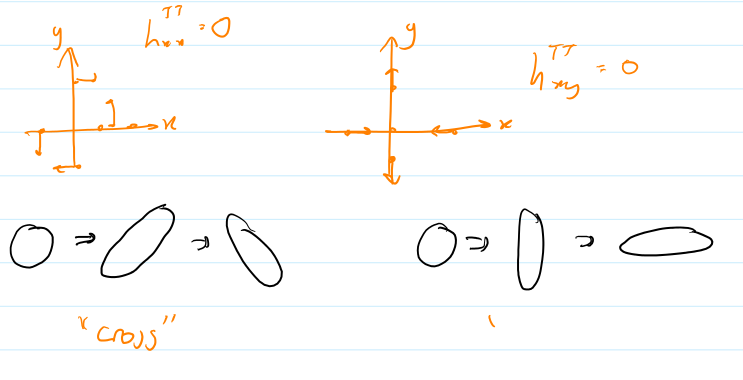
\includegraphics[width=0.7\textwidth]{images/polarisations.png}
\caption{Polarisations}
\end{figure}

Lecture 11/5/16:

\section{LIGO and gravitational wave detection}

\begin{figure}[h]
\centering
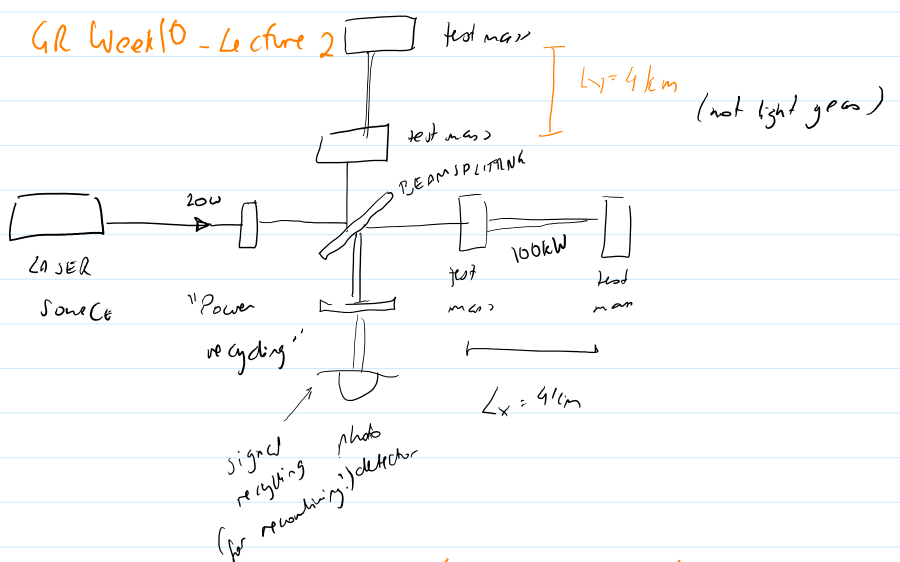
\includegraphics[width=0.6\textwidth]{images/ligo-arms.png}
\caption{LIGO arms}
\end{figure}

Strain is given by
\begin{equation}
\frac{\Delta L}{L}=h
\end{equation}
which is unitless (note: $L$ is the length of an arm). This $h$ is a component of $h_{\mu\nu}$; it is a linear combination of $h_{+}$ and $h_{\times}$, ``cross-polarisation''.

Take $h(t)=\text{strain as a function of time}$;
\begin{align}
h(t)\xrightarrow{\text{Fourier}} h(f)&= \int e^{-2\pi i f(t)}h(t)~dt\\
\underbrace{\text{SNR}}_{\mathllap{\text{signal-to-noise ratio}}}&= \int^{\infty}_{-\infty}df~\frac{|h(f)|^2}{S_n(f)}
\end{align} 
where $|h(f)|^2$ is the power of signal, and $S_n(f)$ is the power of signal noise.

\subsection{Noise spectral density}
An alternative:
\begin{equation}
S_n(f)=(\text{strain noise})^2
\end{equation}

Alternative: let $n(t)$ be noise amplitude vs. time.

Autocorrelation function: $S(\tau)=<n(f)\cap (t+\tau)>$

Then $S_n(f)$ is Fourier transform of $S(\tau)$!

\subsection{LIGO noise sources}
\begin{itemize}
\item Low $f$ - seismic/Newtonian
\item Mid $f$ - thermal
\item High $f$ - shot noise
\item Spikes - resonances
\end{itemize}



\subsection{Detection}

This section is missing; however it only talks about the black hole merger from which they detected gravitational waves, and hence I don't care.

\url{http://arxiv.org/abs/1602.03840}





\section{Relativistic stars}

We consider relativistic stars to be perfect fluids, spherical and spherically symmetric, static and isotropic. Recall that $ds^2$ is given in terms of $g$ as

\begin{equation}
ds^2=g(d\vec{x},d\vec{x})
\end{equation}
\begin{itemize}
\item function of ``radius'' $\vect{x}\cdot \vect{x}=r^2$
\item function of $d\vec{x}$ in an isotropic sense (independent of rotation)
\end{itemize}

i.e.,
\begin{equation}
ds^2 = -F(r)dt^2 + 2E(r)dt~\vect{x}\cdot d\vect{x}'+D(r)(\vect{x}\cdot d\vect{x})^2
+C(r)~d\vect{x}\cdot \vect{x}
\end{equation}
where we find
\begin{equation}
d\vect{x}\cdot d\vect{x}= dr^2+r^2~d\theta^2 + r^2\sin^2\theta \sin^\phi
\end{equation}

Simplify by transformations:
\begin{enumerate}
\item Redefine clocks so $t'=t+\Phi(r)$ (tangle $t$ and $r$ tp get rid of off-diagonal terms)
\item Remove the $dt~dr$ term; choose $\Phi(r)=-\int^r_0 \frac{dr'~r'C(r')}{F(r')}$
\item Redefine radius $r'^2=r^2 C(r)$
\end{enumerate}

We should check that our spacetime interval becomes
\begin{equation}
ds^2=-\underbrace{B(r')}_{\mathclap{e^{2\Phi(r)}}}dt'^2+\underbrace{A(r')}_{\mathclap{e^{2\Lambda(r)}}}dr'^2
+r'^2\left(d\theta^2 + \sin^2\theta~d\phi^2\right)
\end{equation}

We can drop the primes, since only $r'$ terms exist (no $r$ terms).

Substituting into the Einstein field equations:
\begin{align}
G_{tt}&=\frac{1}{r^2}e^{2\Phi}\frac{d}{dr}\left[r\left(1-e^{-2\Lambda}\right)\right]\\
G_{rr}&=-\frac{1}{r^2}e^{2\Lambda}\left(1-e^{-2\Lambda}\right)-\frac{2}{r}\Phi'\\
G_{\theta\theta}&= r^2 e^{-2\Lambda}\left(\Phi''+(\Phi')^2+\frac{\Phi'}{r}-\Phi' \Lambda - \frac{\Lambda'}{r}\right)\\
G_{\phi\phi}&=\sin^2\theta G_{\theta\theta}
\end{align}
where the primes represent derivatives with respect to $r$ (i.e. $\frac{d}{dr}$).

The RHS is stress-energy. Assume a perfect fluid,
\begin{equation}
T=pg + (p+\rho)\vec{u}\otimes \vec{u}
\end{equation}

If star's fluid is static, then $\vec{u}=(u^t,0,0,0)$ and hence $\vec{u}\cdot\vec{u}=-1$ implies $-e^{2\Phi}(u^t)^2=-1$, $u^t = e^{-\Phi}$.

\begin{align}
T_{tt}&=pg_{tt}+(p+\rho)u_t u_t\\
&=-pe^{2\Phi}+(p+\rho)e^{\lambda\Phi}\\
&=\rho e^{2\Phi}
\intertext{note $\rho$ is only present in velocity terms. Remember $\vec{u}=(u^t,0,0,0)$.}
T_{rr}&=rg_{rr}\\
&=p e^{2\lambda}\\
T_{\theta\theta}&=r^2 p\\
T_{\phi\phi}&=r^2 \sin^2 \theta \cdot p
\end{align}

\subsection{Einstein's equations for relativistic star}

Recall, a relativistic star is a spherical ball of perfect fluid, hence its energy-momentum is of a physical sort (has pressure and density).

Today: 
\begin{itemize}
\item we solve this
\item then consider exterior solution if star has finite extent
\end{itemize}

\subsubsection{Metric}
Relativistic stars have the metric
\begin{equation}
ds^2=-e^{2\Phi(r)}dt^2 + e^{2\Lambda(r)}dr^2+r^2d\theta^2 + r^2\sin\theta d\phi^2
\end{equation}
Note $\Phi(r)$ is \underline{not} the Newtonian gravitational potential, but it does reduce to it in the weak field limit.

Recall Einstein's equations\footnote{These are the equations of motions for the field (``curvature'').} gave 3 independent equations: $tt,rr,\theta\theta$. We will evaluate these.

\begin{equation}
tt:\quad\frac{1}{r^2}e^{2\Phi}\frac{d}{dr}\left[r(1-e^{-2\Lambda})\right]=8\pi\rho e^{2\Phi}
\end{equation}
For convenience we replace $\Lambda(r)$ with $m(r)=\frac{r}{2}(1-e^{-2\Lambda})$.
\begin{equation}
\Rightarrow \frac{dm}{dr}=4\pi\rho r^2\label{unknowns1}
\end{equation}

\begin{equation}
rr:\quad -\frac{1}{r}e^{2\Lambda}(1-e^{-2\Lambda})+\frac{2}{r}\Phi'=8\pi p e^{2\Lambda}
\end{equation}

After some substitution and rearrangement,
\begin{equation}
\frac{d\Phi}{dr}=\frac{m+4\pi p r^3}{r(r-2m)}\label{unknowns2}
\end{equation}

The $\theta\theta$ term doesn't give anything extra.

We can use the equation of motion for matter (given the fields, the matter responds and ``moves'' (this also includes motion in the $t$ direction; our star is static); this motion itself affects the fields!):
\begin{equation}
T^{\mu\nu}_{\ph{\mu\nu};\nu}=0
\end{equation}
i.e. energy-momentum conservation.

Radial component: after algevra, with covariant derivative given assumed metric,
\begin{equation}
(\rho+p)\frac{d\Phi}{dr}=-\frac{dp}{dr}\label{unknowns3}
\end{equation}
The other components tell us nothing extra.

We count the unknowns from equations~(\ref{unknowns1}),~(\ref{unknowns2}) and~(\ref{unknowns3}): $m(r),\Phi(r),\rho(r),p(r)$.

So we have 4 unknowns but only 3 equations. However, we also need an equation of state relating $p$ and $\rho$ - this is neither from GR or energy conservation; it is a statistical mechanics property of the fluid.

\subsubsection{The physics}

(\ref{unknowns1}): ``Mass'' continuity relation, i.e. 
\begin{align}
m(r)&=\text{mass enclosed in radius $r$ if $\rho$ is density.}\\
&=\int^r_0~dr'~4\pi r'^2\rho(r')
\end{align}

However,  
\begin{align}
\text{true mass enclosed} &=\int_V d^3\vect{x}~\rho\sqrt{-g}\\
&=\int^r_0 dr'~4\pi r'^2 \rho(r') e^{\Phi(r')+\Lambda(r')} 
\end{align}
where $g$ is the determinant of the metric. This correction is because we must integrate over the \underline{proper volume}.

The correction adjusts for gravitational binding energy.

\HRule

(\ref{unknowns2}): $\frac{d\Phi}{dr}\sim \frac{m}{r^2}$; just like Newton's law for gravitational acceleration, i.e. $\nabla^2 \Phi = 4\pi \rho$, and $\Phi\sim\frac{GM}{r^2}$

However, pressure is also a source of intertia and hence curvature $\Rightarrow$ curvature of spacetime modifies $r^{-2}$ law of gravity.

\HRule

(\ref{unknowns3}): Hydrostatic equilibrium, e.g. Earth's atmosphere etc., $\rho\times\underbrace{\text{(gravitational acceleration)}}_{\mathclap{\text{vector}}}=-\nabla p$

However, pressure also gravitates, i.e. inertia of fluid includes its pressure.

\HRule

We recall 
\begin{align}
\frac{dm}{dr}&=4\pi r^2 \rho\\
\frac{d\Phi}{dr}&=\frac{m+4\pi \rho r^3}{r(r-2m)}
\end{align}

Suppose star has fininte extent: $\rho=p=0$ for $r\geq R$.

Exterior: 
\begin{itemize}
\item $m=$ constant (call it $M$)
\item $\frac{d\Phi}{dr}=\frac{m}{r(r-2m)}$
\end{itemize}

Integrate:
\begin{equation}
2\Phi=\ln \left(1-\frac{2m}{r}\right)
\end{equation}

Substitute for $\Phi$ and $\Lambda$ in original metric:
\begin{equation}
ds^2=-\left(1-\frac{2m}{r}\right)dt^2+\left(1-\frac{2m}{r}\right)^{-1}dr^2 + r^2 d\theta^2
+r^2\sin^2 \theta~d\phi^2
\end{equation}

This is the Schwarzchild metric! (which we have now derived). It is the exterior metric for \underline{any} spherically symmetric mass distribution (Birkhoff's therorem).

What happens to an astronaut orbiting a BH?

Assume free fall: solve geodesic equations $\nabla_{\vec{u}}\vec{u}=0$. \footnote{If not in free fall, i.e. rockets turned on, we solve $\nabla_{\vec{u}}\vec{u}=\vec{a}$ and infer $\vec{a}$ in terms of proper acceleration. We will not consider this case.}

Note that  $\nabla_{\vec{u}}\vec{u}=0$ also implies $\nabla_{\vec{u}}\tilde{u}=0$.

We already proved: $\frac{du_{\alpha}}{d\tau}=\frac{1}{2}g_{\mu\nu,\alpha}u^{\mu} u^{\nu}$.

Schwarz: metric independent of $t$ and $\phi \Rightarrow u_t$ and $u_{\phi}$ are constants.

We call
\begin{itemize}
\item $u_t=-E$\quad energy/mass at infinity
\item $u_{\phi}=L$\quad angular momentum/mass at infinity (component along z-axis)
\end{itemize}

We can also prove (see various books) orbit of particle is confined to a plane (like Newtonian).

i.e., 
\begin{align}
u^{\theta}&=\frac{d\theta}{d\tau}=0 \text{ and hence } u_{\theta}=g_{\theta\theta}u^{\theta}=0
\intertext{Take $\theta=\frac{\pi}{2}$ (equatorial)}
u^t&=g^{tt}u_t=E\left(1-\frac{2m}{r}\right)^{-1}\\
u^{\phi}&=g^{\phi\phi}u_{\phi}=\frac{L}{r^2}
\end{align}

Equation of motion for $u^r$: equivalently take $r$ component of $\nabla_{\vec{u}}\vec{u}=0$ \underline{or} recall normalisation $\vec{u}\cdot\vec{u}=-1$.

\begin{align}
-1&=g_{tt}(u^t)^2+g_{rr}(u^r)^2+0+g_{\phi\phi}(u^{\phi})^2\\
&=-\left(1-\frac{2m}{r}\right)\cdot E^2 \left(1-\frac{2m}{r}\right)^{-2}+\left(1-\frac{2m}{r}\right)^{-1}(u^r)^2+r^2\cdot \left(\frac{L}{r^2}\right)^2\\
\text{i.e., }\left(\frac{dr}{d\tau}\right)^2&=E^2-
\underbrace{\left(\frac{L^2}{r^2}+1\right)\left(1-\frac{2M}{r}\right)}_{\mathclap{V_{\text{eff}}(r)^2}}
\end{align}
Orbit only exists if $E \geq V_{\text{eff}}$


\begin{figure}[h]
\centering
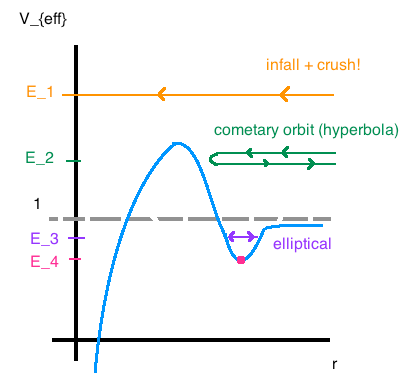
\includegraphics[width=0.6\textwidth]{images/v_eff-orbit.png}
\caption{Various orbit types}
\end{figure}

Circular: $\frac{dV_{\text{eff}}}{dr}=0$.
\begin{equation}
r=\frac{L^2}{2M}\left(1+\sqrt{1-\frac{12M^2}{L^2}}\right)
\end{equation}

Unlike Newtonian mechanics, a circular orbit only exists for $L^2 12M^2$. Small circular orbit:
\begin{equation}
r=\frac{12M^2}{2M}=6M.
\end{equation}
$\Rightarrow$ ISCO = innermost stable circular orbit.

\HRule

Lecture 19-5-16:

\section{Photons}

Consider the 4-momentum of a photon
\begin{equation}
\vec{p} \propto \frac{d\vec{x}(\lambda)}{d\lambda}
\end{equation}
where $\lambda$ is the affine parameter.

\begin{equation}
p_\tau = -E,\quad p_{\phi}=L,\quad p_{\theta}=0
\end{equation}
all constants.

We have the normalisation $\vec{p}\cdot \vec{p}=0$ for a null ray.

Consider:
\begin{equation}
\left(\frac{dr}{d\lambda}\right)^2=E^2 - \underbrace{\frac{L^2}{r^2}\left(1-\frac{2M}{r}\right)}_{V_{\text{eff}}^2}
\end{equation}
where $L$ is angular momentum. To find $R$, we maximise $V_{\text{eff}}$ then can solve for $R$.


\HRule


\subsection{Perihelion advance of Mercury}


``You may not know this, but Mercury really is a potato."

\begin{figure}[h]
\centering
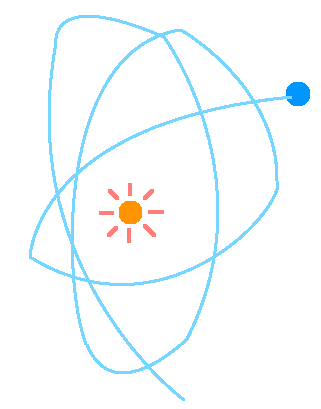
\includegraphics[width=0.4\textwidth]{images/perihelion-of-mercury.png}
\caption{Perihelion precession}
\end{figure}

Where could this come from? 
\begin{itemize}
\item torques from other planets
\item spin-orbit coupling (Mercury is a potato; 2:3 resonance
\item change in 43'' per century; unexplainined in early 1900's (a planet ``Vulcan'' was predicted)
\end{itemize}

GR (Einstein) predicted: gravitational acceleration around mass $M$ is \underline{not} simply $-\frac{M}{r^2}$; correction like $-\frac{M}{r^2}\frac{1}{1-\frac{2M}{r}}$ (approx.).

Special case: potential $\propto r^2$ \underline{or} $r^{-1}$ leads to \underline{closed} bound orbits. All other potentials do not!

i.e., GR corrections leads to precession.

To calculate this, we need $r(\phi)$ or equivalently $\phi(r)$. From previous lectures we have $\frac{dr}{d\tau},\frac{d\phi}{d\tau}$.

\begin{align}
\Rightarrow \frac{dr}{d\phi}&=\frac{dr}{d\tau}\times\left(\frac{d\phi}{d\tau}\right)^{-1}\\
\text{Let } u&=\frac{1}{r}\quad\text{(just for convenience)}\\
\left(\frac{du}{d\phi}\right)^2&=\frac{E^2}{L^2}-(1-2Mu(\left(\frac{1}{L^2}+u^2\right)\label{du dphi}
\end{align}
In the Newtonian case: ignore $y^3$ term (GR).

Circular orbit has $u=\dfrac{M}{L^2}=$ constant.

So we have deviation from circularity as:
\begin{equation}
y=u-\frac{M}{L^2}
\end{equation}

\begin{figure}[h]
\centering
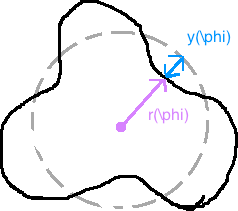
\includegraphics[width=0.3\textwidth]{images/dev-from-circularity.png}
\caption{Deviation from circularity of an orbit}
\end{figure}

Substituting this into~(\ref{du dphi});
\begin{equation}
\left(\frac{dy}{d\phi}\right)^2=\frac{E^2-1}{L^2}+\frac{M^2}{L^4}-y^2
+\underbrace{\frac{2M^4}{L^6}+\frac{6M^3 y}{L^2}+\frac{6M^2}{L^2}y^2}_{GR}
\end{equation}

The non-GR bit has a colution
\begin{equation}
y=A\cos(\phi+\phi_0)
\end{equation}
This has period $2\pi$.

GR bit has solution:
\begin{equation}
y=A\cos\left[\left(1-\frac{6M^2}{L^2}\right)\phi + \phi_0\right]
\end{equation}

There is a mismatch between the period of $y$ and orbitial period ($2\pi$).
\begin{equation}
\text{Perihelion shift per orbit}=2\pi - \frac{2\pi}{1-\frac{6M^2}{L^2}}
\end{equation}

\exercise{Show that this equals the expected 43'' per century.}{}


\section{Black holes}
\subsection{Kerr black holes}


A Kerr blackhole is a source with mass $M$ and angular momentum $J=aM$ ($a< 1$).

Metric is given in Schutz. It is distinguished by $g_{t\phi}=g_{\phi t}\neq 0$ (off-diagonal element). The metric is independent of $t$ and $\phi \Rightarrow u_t$ and $u_{\phi}$ are constants on any free-fall orbit.

\begin{align}
u^t&=g^{tt} u_t + g^{t\phi}u_{\phi}\\
u^{\phi}&= g^{t\phi}u_t + g^{\phi\phi} u_{\phi}
\end{align}

Suppose we drop a particle from $\infty$ directly (radially) into the centre of a Kerr BH (free-fall). Zero angular momentum at infinity $\Rightarrow u_{\phi}=0=\text{ constant}$.

At radius $r<\infty$:
\begin{equation}
\text{Angular velocity in global coordinates}=\frac{d\phi}{dt}=\frac{u^{\phi}}{u^t}
=\frac{g^{t\phi}u_t}{g^{tt}u_t}=\frac{g^{t\phi}}{g^{tt}}\neq 0
\end{equation}

i.e., a particle is dragged into rotation by the rotating spacetime around a BH. This \textbf{frame dragging} leads to Lense-Thirring precession of a gyroscope.

\subsubsection{Kerr ergosphere and horizon}

Suppose we have a photon on a circular orbit in equatorial plane (in a Schwarzchild, and also Kerr, space: circular orbit is unstable for photons; we need mirrors!).

\begin{figure}[h]
\centering
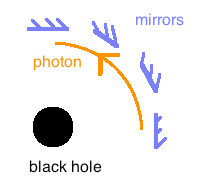
\includegraphics[width=0.3\textwidth]{images/photon-BH-mirrors.png}
\caption{Mirrors around a BH to maintain photon orbit}
\end{figure}

\begin{align}
ds^2&=0 \quad\text{(null ray)}\\
&=g_{tt}dt^2 + 2g_{t\phi} dt~d\phi + g_{\phi\phi} d\phi^2
\intertext{noting that $dr=d\theta=0$ on a null ray.}
\Rightarrow \frac{d\phi}{dt}&=\frac{-2g_{t\phi}\pm \sqrt{4g_{t\phi}^2-4g_{tt}g_{\phi\phi}}}{2}
\end{align}
This means that for our photon, two angular velocities (in global coordinates) are possible. This is due to frame dragging (prograde - rotating with BH - and retrograde - rotating against the BH - are not symmetric).

Like with Schwarzchild: a radius exists where $g_{tt}=0$. This radius is the \underline{horizon}. At this radius:
\begin{equation}
\frac{d\phi}{dt}=-2g_{t\phi}\text{ \underline{or} zero!}
\end{equation}
depending on whether motion is with or against BH rotation. A retrograde photon makes no ``headway'' against frame dragging (while a prograde photon would be ``helped along'')!

Schutz gives the radius of the ergosphere as
\begin{equation}
r_{\text{ergo}}=M+\sqrt{M^2+a^2\cos^2\theta}
\end{equation}

Note: this is all in global coordinates! If instead we were in a local reference frame, the photon would be travel at $c$.

\subsection{Black hole coordinates}
We will use a Schwarzchild example, using the standard $(t,r,\theta,\phi)$.

Define new coordinates: stretch radial coordinates
\begin{equation}
(r,t)\mapsto (r,\tilde{V})
\end{equation}
with
\begin{equation}
\tilde{V}=t+\underbrace{r^{\ast}}_{\mathclap{\text{tortoise coordinate}}}=t+r+2M\ln\left|\frac{r}{2M}-1\right|
\end{equation}

Why is this form useful?
\begin{align}
\frac{dr^{\ast}}{d\tau}&=\frac{dr}{d\tau}+\frac{2M}{\frac{r}{2M}-1}
\cdot\frac{1}{2M}\frac{dr}{d\tau}\\
\text{i.e.,}\quad dr^{\ast}&=\frac{dr}{1-\frac{2M}{r}}
\end{align}
This is useful for ``killing'' (removing) the divergent factor (as $r\to 2M$) in standard Schwarzchild.

We also transform the metric (left as exercise):
\begin{equation}
ds^2 = -\left(1-\frac{2M}{r}\right) d\tilde{V}^2 + 2d\tilde{V}~dr+r^2~d\Omega^2
\end{equation}
called Eddington-Finkelstein coordinates.

Considering the light-cone now: $ds^2=0$. Fix $d\Omega^2=0$.
\begin{equation}
\therefore \frac{d\tilde{V}}{dr}=0\quad\text{and}\quad \frac{2}{1-\frac{2M}{r}}
\end{equation}
Two edges of the light cone.

\begin{figure}[h]
\centering
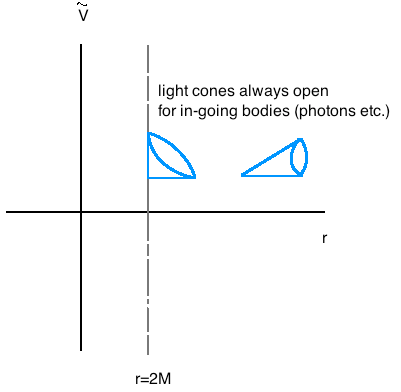
\includegraphics[width=0.5\textwidth]{images/ef-lightcone.png}
\caption{EF lightcone}
\end{figure}

\begin{figure}[h]
\centering
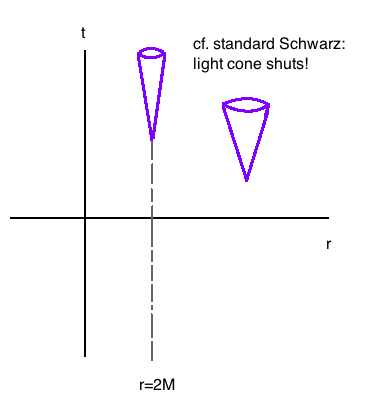
\includegraphics[width=0.5\textwidth]{images/schwarz-lightcone.png}
\caption{Schwarzchild lightcone}
\end{figure}


Also exists: Eddington-Finkelstein \underline{outgoing}

\begin{equation}
(r,t)\mapsto (r,\tilde{U})\quad\text{with }\tilde{U}=t-r^{\ast}
\end{equation}
\exercise{?}{Calculate the light cone}.

\HRule

Can we combine these so that the event horizon is regularised for \underline{all} (both going in \underline{or} out) particles?

Let's try:
\begin{align}
(t,r) &\mapsto (\tilde{U},\tilde{V})\\
\tilde{V}-\tilde{U}&=2r^{\ast}\\
\tilde{V}+\tilde{U}&= 2t
\end{align}

We transform the metric as usual (do this as an exercise):
\begin{equation}
ds^2 = -\left(1-\frac{2M}{r}\right) d\tilde{U}~d\tilde{V}+r^2~d\Omega^2
\end{equation}
Sadly this still leads to an event horizon at $r=2m$. e.g. consider a stationary observer and use $\vec{u}\cdot \vec{u}=-1$ to show that the component blows up.

But luckily, we see form the definition:
\begin{align}
e^{r^{\ast}/2M}&=e^{r/2M}\left(\frac{r}{2M}-1\right)\\
\text{i.e.,}\quad e^{(\tilde{V}-\tilde{U})/4M}&= e^{r/2M}\left(\frac{r}{2M}-1\right)
\end{align}

We try relabelling:
\begin{equation}
\tilde{u}=-e^{-\tilde{U}/4M}\quad\text{and}\quad \tilde{v}=e^{\tilde{V}/4M}
\end{equation}
Transform metric (as usual):
\begin{equation}
ds^2 = -\frac{32M^3}{r}e^{-r/2M}~d\tilde{u}~d\tilde{v}+r^2~d\Omega^2
\end{equation}
i.e.
\begin{equation}
g_{\tilde{u}\tilde{u}}=0=g_{\tilde{v}\tilde{v}}
\end{equation}
Now looking at this, we have no event horizon at $r=2M$! Only the essential singularity is left! (at $r=0$; this is singularity is unavoidable and cannot be removed by clever methods)

The ``singularity'' we had at the event horizon is not actually physical - an astronaut passing through it would not feel anything ``singular''!

\subsubsection{Kruskal-Szekeres}
\begin{align}
\text{Let }u&=\frac{1}{2}(\tilde{v}-\tilde{u})\\
v&=\frac{1}{2}(\tilde{v}+\tilde{u})\\
ds^2&=-\frac{32M^3}{r}e^{-r(u,v)/2M)}(dv^2 - du^2) + r^2~d\Omega^2
\end{align}

In these coordinates, the lightcone is: $v = \pm u$, which is just like in Minkowski!

The central singularity ($r=0$) corresponds to $v^2 - u^2 = 1$.

\begin{figure}[h]
\centering
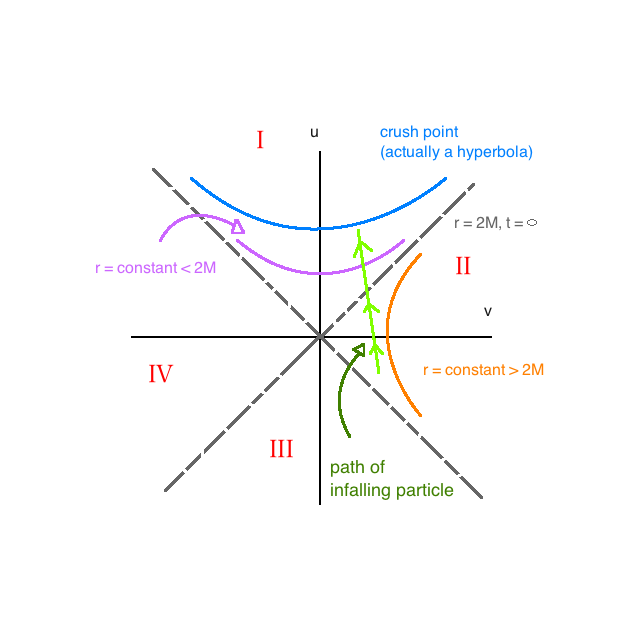
\includegraphics[width=0.6\textwidth]{images/ks-coords.png}
\caption{Kruskal-Szekeres coordinates}
\end{figure}
Standard Schwarz = I union II, \underline{or} III union IV.

i.e. Schwarzchild standfard coordinatec over only \underline{half} the manifold!! (cf. twin paradox).

\section{Global methods}
MTW ch. 34 as starting point.

Aim: ``compactify'' the manifold, i.e. introduce coordinatrs with fininte values at $\infty$.

e.g., flat: 
\begin{equation}
ds^2 = -dt^2 + dr^2 + r^2~d\Omega^2
\end{equation}

\begin{align}
\text{Let } t+r&=\tan\frac{\psi+\xi}{2}\\
t-r&= \tan \frac{\psi-\xi}{2}
\end{align}
So that the transformed metric becomes
\begin{equation}
ds^2=\frac{-d\psi^2 + d\xi^2}{4\cos^2\frac{\psi+\xi}{2}\cos^2\frac{\psi-\xi}{2}}+r^2~d\Omega^2
\end{equation}

\begin{figure}[h]
\centering
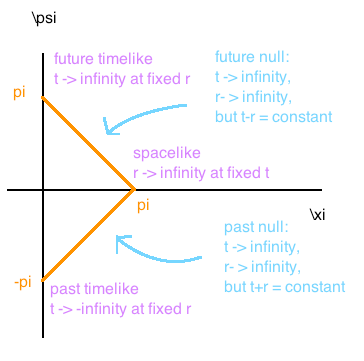
\includegraphics[width=0.6\textwidth]{images/global-methods.png}
\caption{Global methods}
\end{figure}

\section{Cosmology}
(the last lecture, apparently)

The universe is homogenous and isotropic.

\begin{itemize}
\item Homogenous - (the geometry of spacetime is the) same at every point
\item Isotropic - same in every direction, as viewed from every point
\end{itemize}

These qualities are empirical! There is no reason for the universe to have these properties.
\begin{itemize}
\item only true at the largest scales
\item cosmic microwave background (blackbody temperature is smooth to $\sim 10^{-6}$
\item large-scale strcutre - maps of galaxy distribution in sku
\item inhomoegenous models
\begin{itemize}
\item Swiss Cheese model
\item recent papers by Bolejko et. al.
\item David Wiltshire's papers
\end{itemize}
\end{itemize}

\subsection{Metric}
Divide spacetime into constant-$t$ 3D hypersurfaces. Define $t$ to be the proper time at any 3D point (associated co-moving volume) (``galaxy'').

In each hypersurface:
\begin{align}
d\l^2_{\text{3D}}&= h_{ij}(t)~dx^i ~ dx^j , \quad\text{homogeneous}\\
&=\underbrace{R(t)^2}_{\mathclap{\text{scale factor}}} h_{ij}(t=0)~dx^i ~ dx^j
\intertext{To \underline{maintain} isotropy (not to establish isotropy in the first place). A spatial interval of \underline{any} orientation expands/contracts with $t$ at the same rate.}
&= R(t)^2 \left[e^{2\Lambda(r)}dr^2 + r^2~d\Omega\right]
\end{align}

Isotropy (symmetric w.r.t. point rotations like Schwarzschild).

Also,
\begin{itemize}
\item $t$ proper time (at $dx^i ~ dx^j = 0$) $\Rightarrow$ $-dy^2$ term
\item no cross terms $dt~dx^i$ because:
\begin{enumerate}
\item proper time $t$ = coordinate time $t$
\item time reversal symmetry
\item reflection symmetry $\vect{x}\mapsto -\vect{x}$
\end{enumerate}
\end{itemize}

\begin{equation}
ds^2 = -dt^2 + R(t)^2 \left[e^{2\Lambda(r)}~dr^2 + r^2~d\Omega\right]
\end{equation}

Homogenous means, among other things, that the Ricci scalar is uniform. Form previous lectures on relativistic stars (check as an exercise)
\begin{equation}
\frac{1}{r^2}\frac{d}{dr}\left[r(1-e^{-2\Lambda})\right]=\text{constant}
\end{equation}
from $G_{tt}$ components. Integrating this,
\begin{equation}
e^{2\Lambda}=\frac{1}{1-kr^2}
\end{equation}
where $k$ is a constant. Boundary condition: metric is flat (i.e. $e^{2\Lambda(r)}=1$) at $r=0$). This looks like it is bad (i.e. we have chosen a ``special point'' and requiring space to be flat at one point, but no constraint elsehwere). However, $r=0$ is \underline{not} a special point! We can arbitrarily choose any point.

We can always rescale $r$ so that
\begin{equation}
k = \begin{cases}
-1 & \text{open}\\
0 & \text{flat} \\
1 & \text{closed}
\end{cases}
\end{equation}

The Friedman-Robertson-Walker metric is:
\begin{equation}
ds^2 = -dt^2 + R(t)^2 \left[\frac{dr^2}{1-kr^2}+r^2~d\Omega\right]
\end{equation}

Substitute into Einstein's equations (LHS) and get derivatives of $R(t)$. 

RHS of Einstein: $T^{\mu\nu}$ includes $\underbrace{\text{baryons, photons, leptons, $\ldots$}}_{\text{different equations of state $p=p(\rho)$}}$

Solve this to get $R(t)$. This gives the history and future of the Universe!



%-------------------------------------------------------
\pagebreak
\part{Appendix}

\setcounter{section}{0}
Indices up = vector-like

Indices down = 1-form-like

\section{Covariant derviative notation}
\subsection{Vectors}
We realise that the component form of $\nabla \vec{V}$ can be written as $(\nabla \vec{V})^{\alpha}_{\beta}$.

\begin{equation}
\underbrace{(\nabla \vec{V})^{\alpha}_{\beta}}_{\text{notation: }V^{\alpha}_{;\beta}}=
\underbrace{\frac{\partial V^{\alpha}}{\partial x^{\beta}}}_{\text{notation: }V^{\alpha}_{,\beta}}
+\Gamma^{\alpha}_{\lambda\beta}V^{\lambda}
\end{equation}

That is:
\begin{align}
V^{\alpha}_{,\beta}&:=\frac{\partial V^{\alpha}}{\partial x^{\beta}}\\
(\nabla \vec{V})^{\alpha}_{\beta}\equiv V^{\alpha}_{;\beta}&:=V^{\alpha}_{,\beta}+\Gamma^{\alpha}_{\lambda\beta}V^{\lambda}
\end{align}

\subsection{One-forms}
Components of $\nabla\tilde{p}$, i.e. $(\nabla\tilde{p})_{\alpha\beta}$ is notationally $p_{\alpha;\beta}$

\begin{equation}
p_{\alpha;\beta}=\frac{\partial p_{\alpha}}{\partial x^{\beta}}-\Gamma^{\lambda}_{\alpha\beta} p_{\lambda}
\end{equation}

\subsection{General tensors}
For general tensor: add correction term $\pm \Gamma$ tensor for each tensor index; $+$ is index is up; $-$ if index is down.

\begin{equation}
\text{e.g. }\quad T^{\alpha}_{\beta;\gamma}=\frac{\partial T^{\alpha}_{\beta}}{\partial x^{\gamma}}
+\underbrace{\Gamma^{\alpha}_{\lambda\gamma} T^{\lambda}_{\beta}}_{\text{by analogy with vector}}
-\underbrace{\Gamma^{\lambda}_{\beta \gamma}T^{\alpha}_{\lambda}}_{\text{by analogy with 1-form}}
\end{equation}

\begin{equation}
\nabla_{\vec{u}}\vec{v}=(\nabla\vec{v})\cdot \vec{u}
\end{equation}
...probably?


\subsection{Metric}
In flat space, $g_{\alpha\beta , \gamma}=0$ \underline{and} $\Gamma$'s are zero because $\frac{\partial\vec{e}_{\alpha}}{\partial x^{\beta}}=0$
\begin{align}
\Rightarrow g_{\alpha\beta;\gamma}&=g_{\alpha\beta,\gamma}-(\text{two terms involving Christoffel symbols})\\
&=0 \quad\text{in flat space}
\end{align}

%-----------------------------------------


\end{document}



